%% LyX 1.3 created this file.  For more info, see http://www.lyx.org/.
%% Do not edit unless you really know what you are doing.
\documentclass[english, 12pt]{article}
\usepackage{times}
%\usepackage{algorithm2e}
\usepackage{url}
\usepackage{bbm}
\usepackage[T1]{fontenc}
\usepackage[latin1]{inputenc}
\usepackage{geometry}
\geometry{verbose,letterpaper,tmargin=2cm,bmargin=2cm,lmargin=1.5cm,rmargin=1.5cm}
\usepackage{rotating}
\usepackage{color}
\usepackage{graphicx}
\usepackage{subcaption}
\usepackage{amsmath, amsthm, amssymb}
\usepackage{setspace}
\usepackage{lineno}
\usepackage{hyperref}
\usepackage{bbm}
\usepackage{makecell}

%\renewcommand{\arraystretch}{1.8}

%\usepackage{xr}
%\externaldocument{SCT-supp}

%\linenumbers
%\doublespacing
\onehalfspacing
%\usepackage[authoryear]{natbib}
\usepackage{natbib} \bibpunct{(}{)}{;}{author-year}{}{,}

%Pour les rajouts
\usepackage{color}
\definecolor{trustcolor}{rgb}{0,0,1}

\usepackage{dsfont}
\usepackage[warn]{textcomp}
\usepackage{adjustbox}
\usepackage{multirow}
\usepackage{graphicx}
\graphicspath{{figures/}}
\DeclareMathOperator*{\argmin}{\arg\!\min}

\let\tabbeg\tabular
\let\tabend\endtabular
\renewenvironment{tabular}{\begin{adjustbox}{max width=0.9\textwidth}\tabbeg}{\tabend\end{adjustbox}}

\makeatletter

%%%%%%%%%%%%%%%%%%%%%%%%%%%%%% LyX specific LaTeX commands.
%% Bold symbol macro for standard LaTeX users
%\newcommand{\boldsymbol}[1]{\mbox{\boldmath $#1$}}

%% Because html converters don't know tabularnewline
\providecommand{\tabularnewline}{\\}

\usepackage{babel}
\makeatother


\begin{document}


\title{Efficient toolkit implementing best practices for principal component analysis of population genetic data}
\author{Florian Priv\'e,$^{\text{1,5,}*}$ Keurcien Luu$^{\text{5}}$, Michael G.B. Blum,$^{\text{4,5}}$ John J. McGrath,$^{\text{1,2,3}}$ and Bjarni J. Vilhj\'almsson$^{\text{1,}*}$}

\date{~ }
\maketitle

\noindent$^{\text{\sf 1}}$National Centre for Register-Based Research, Aarhus University, Aarhus, 8210, Denmark. \\
\noindent$^{\text{\sf 2}}$Queensland Brain Institute, University of Queensland, St. Lucia, 4072, Queensland, Australia. \\
\noindent$^{\text{\sf 3}}$Queensland Centre for Mental Health Research, The Park Centre for Mental Health, Wacol, 4076, Queensland, Australia. \\
\noindent$^{\text{\sf 4}}$OWKIN France, Paris, 75010, France. \\
\noindent$^{\text{\sf 5}}$Laboratoire TIMC-IMAG, UMR 5525, Univ.\ Grenoble Alpes, La Tronche, 38700, France. \\
\noindent$^\ast$To whom correspondence should be addressed.\\

\noindent Contacts:
\begin{itemize}
\item \url{florian.prive.21@gmail.com}
\item \url{bjv@econ.au.dk}
\end{itemize}

\newpage

\abstract{
Principal Component Analysis (PCA) of genetic data is routinely used to infer ancestry and control for population structure in various genetic analyses. However, conducting PCA analyses can be complicated and has several potential pitfalls. These pitfalls include (1) capturing Linkage Disequilibrium (LD) structure instead of population structure, (2) projected PCs that suffer from shrinkage bias when projecting PCA from a reference dataset to another independent dataset, (3) detecting sample outliers, and (4) uneven population sizes. In this work, we explore these potential issues when using PCA, and present efficient solutions to these. Following applications to the UK Biobank and the 1000 Genomes project datasets, we make recommendations for best practices and provide efficient and user-friendly implementations of the proposed solutions in R packages bigsnpr and bigutilsr.

For example, we show that PC19 to PC40 in the UK Biobank capture LD structure. Using our automatic algorithm for removing long-range LD regions, we recover 16 PCs that capture population structure only.
Therefore, we recommend using only 16-18 PCs from the UK Biobank. 
We provide evidence for a shrinkage bias when projecting PCs computed with data from the 1000 Genomes project.  Although PC1 to PC4 suffer from only moderate shrinkage (1.01-1.09), PC5 (resp.\ PC10) for example suffers from a shrinkage factor of 1.50 (resp.\ 3.14). 
We provide a fast way to project new individuals that is not affected by this shrinkage bias. 
We also show how to use PCA to restrict analyses to individuals of homogeneous ancestry. 

Overall, we believe this work would be of interest for anyone using PCA in their analyses of genetic data, as well as for other omics data.
}


%%%%%%%%%%%%%%%%%%%%%%%%%%%%%%%%%%%%%%%%%%%%%%%%%%%%%%%%%%%%%%%%%%%%%%%%%%%%%%%%

\newpage

\section{Introduction}

Principal Component Analysis (PCA) has been widely used in genetics for many years and in many contexts. For instance, adding PCs as covariates has been routinely used to adjust for population structure in Genome-Wide Association Studies (GWAS) \cite[]{price2006principal,novembre2008interpreting}. PCA has also been used to detect loci under selection \cite[]{galinsky2016fast,luu2017pcadapt}.
Recently, the advent of large population-scale genetic datasets, such as the UK biobank data, has prompted research on developing scalable algorithms to compute PCA on very large data \cite[]{bycroft2017genome}.
It is now possible to efficiently approximate PCA on very large datasets thanks to software such as FastPCA (fast mode of EIGENSOFT), FlashPCA2, PLINK 2.0 (approx mode), bigstatsr/bigsnpr, TeraPCA and ProPCA \cite[]{galinsky2016fast,abraham2017flashpca2,chang2015second,prive2017efficient,bose2019terapca,agrawal2019scalable}.

However, some pitfalls related to PCA of genotype data have been documented and not all of the currently available software address all of these. 
In the following, we outline common pitfalls and explain when they are relevant.
First, some of the PCs may capture LD structure rather than population structure \cite[]{price2008long,abdellaoui2013population,prive2017efficient}. Including PCs that capture LD as covariates in genetic analyses can lead to reduced power, e.g.\ for detecting genetic association within these LD regions in GWAS.  
Second, another issue may arise when projecting PCs of a reference dataset to another study dataset: projected PCs are shrunk towards 0 in the new dataset \cite[]{lee2010convergence,wang2015improved,zhang2019fast}. This shrinkage makes it potentially dangerous to use the projected PCs for analyses such as PC regression, ancestry detection and correction for ancestry.
Third, PC scores may capture outliers that are due to family structure, population structure or other reasons; it might be benificial to detect and remove these individuals to maximise the population structure captured by PCA (in the case of removing a few outliers) or to restrict analyses to genetically homogeneous samples (e.g.\ ``White British'' people in the UK Biobank).
Finally, efficient methods for PCA use approximations, which can results in some lack of precision of computed PCs. This has been shown to be a possible issue for software such as FastPCA and PLINK 2.0, but not for FlashPCA2 and bigstatsr/bigsnpr \cite[]{abraham2017flashpca2,prive2017efficient}.
An overview of existing methods with their respective advantages and limitations is presented in table \ref{tab:method-overview}.

For this paper, we derive implementations of truncated PCA and other useful functions for e.g.\ performing LD thinning and computing variant statistics. We make these available in a new release of R package bigsnpr (v1.0.0); what differs from previously available functions presented in \cite{prive2017efficient} is that these new functions can be used directly on PLINK bed/bim/fam files with some missing values. 
We use these new functions to analyse the UK Biobank data, and show that they are both very fast and easy to use. We also point out that many PCs currently reported by the UK Biobank capture LD structure instead of population structure. Interestingly, subsetting the UK Biobank data enables to get more PCs capturing population structure than when using the whole sample (\textasciitilde40 instead of \textasciitilde16).
Then, we project the other individuals that were not used in the PCA calculation, show that this projection is biased and provide an efficient solution to estimate unbiased projections instead.
Finally, we explore options to detect outlier samples in PCA, either a few outlier samples that may correspond to e.g.\ batch effects, or when the goal is to restrict the data to individuals of homogeneous ancestry.

%%%%%%%%%%%%%%%%%%%%%%%%%%%%%%%%%%%%%%%%%%%%%%%%%%%%%%%%%%%%%%%%%%%%%%%%%%%%%%%%

\section{Material and Methods}

\begingroup
\renewcommand*{\arraystretch}{2}
\begin{table}[h]
\centering
\caption{Overview of existing methods.} 
\label{tab:method-overview}
\begin{tabular}{|c|c|c|c|c|}
\hline
Analysis & Method and/or Software & Citation & Advantages & Limitations \\
\hline
\multirow{3}{*}{PCA} & bigstatsr / bigsnpr & \cite[]{prive2017efficient} & \makecell{Fast and accurate + handle dosages \\ + thinning options directly included} & \makecell{Own format without missing values \\ (fast functions are available \\ for converting and imputing)} \\
 & FlashPCA2 & \cite[]{abraham2017flashpca2} & Fast and accurate & Not parallelised \\
 & PLINK 2.0 (reimplementation of FastPCA) & \cite[]{galinsky2016fast,chang2015second} & Fast & \makecell{Possible lack of accuracy \\ \cite[]{abraham2017flashpca2,prive2017efficient}} \\
\hline
\makecell{Detection of \\ oultier samples} & \makecell{``6 SDs from the mean'' \\ in EIGENSOFT} & \cite[]{patterson2006population} & Simple & Assumes Gaussian distritbution \\
\hline
\makecell{Detection of \\ homogeneous \\ samples} & R package aberrant & \cite[]{bellenguez2011robust} & Robust & Only two statistics at once \\
\hline
\multirow{5}{*}{\makecell{Projection of \\ new individuals \\ onto reference \\ PCA space}} & Simple projection (multiplication by loadings) & & Simple & Shrinkage biased \\
  & Bias-adjusted projection in R package hdpca & \cite[]{dey2019asymptotic} & Independent of new samples & \makecell{Assumes same shrinkage for all individuals \\ + model-based \\ + need all eigenvalues of reference} \\
  & \makecell{Augmentation, Decomposition and Procrustes (ADP) \\ transformation in LASER 2.0} & \cite[]{wang2015improved} & Accurate & Slow (a new PCA for each new sample) \\
  & Online ADP (OADP) in python package FRAPOSA & \cite[]{zhang2019fast} & Much faster than ADP & Does not work for related individuals (Section \ref{proj-related}) \\ 
\hline
\end{tabular}
\end{table}
\endgroup

\subsection{Efficient implementation of PCA for genotype data}

When there is no missing value, we compute the partial Singular Value Decomposition (SVD) $U \Delta V^T$ of the scaled genotype matrix of diploid individuals $\tilde{G}_{i,j} = \frac{G_{i,j} - 2 \hat{f_j}}{\sqrt{2 \hat{f_j} (1 - \hat{f_j})}}$ where $G_{i,j}$ is the allele count (genotype) of individual $i$ and variant $j$, and $\hat{f_j}$ is the estimated allele frequency of variant $j$ ($2 \hat{f_j}$ is the mean allele count of variant $j$). Then, $U \Delta$ are the first $K$ PC scores and $V$ are the first $K$ PC loadings, where $K$ is the number of PCs computed (e.g.\ $K=20$).

When there are some missing values, we compute the partial SVD similarly, except that missing values are replaced by the variant means (i.e.\ $G_{i,j} - 2 \hat{f_j} = 0$ when $G_{i,j}$ is missing) and  the $\hat{f_j}$ for each variant are estimated using only non-missing values of each variant.
Note that this decomposition is equivalent to the decomposition presented above after imputation by the variant means.

To compute this decomposition easily and efficiently, we implement an accessor that memory-map the PLINK bed file to use it directly as if it were a standard matrix. Then, we apply the same algorithm for partial SVD that is used in R packages bigstatsr and FlashPCA2, namely the implicitly restarted Arnoldi method \cite[]{Lehoucq1996,abraham2017flashpca2,prive2017efficient}. 
This algorithm is implemented in R package RSpectra, and requires a function that computes the matrix-vector multiplication of the scaled genotype matrix with a given vector, which we implement for PLINK bed files and parallelise.

\subsection{Robust Mahalanobis distance \label{maha}}

Mahalanobis distances are computed as $d(x)^2 = (x-\mu)^T \Sigma^{-1} (x-\mu),$ where $\mu$ and $\Sigma$ are (robust) estimators of location and covariance of $x$.
We use these distances for many applications in this paper. 
When $x$ is multivariate Gaussian data with $K$ dimensions, the squared distances follow a $\chi^2(K)$ distribution.
If $x$ are PC scores of centered data and if we use standard estimates, then $\mu = 0$ and $\Sigma = I_K$.
Yet, here we use the pairwise orthogonalised Gnanadesikan-Kettenrin robust estimates of these parameters, as implemented in function \texttt{covRob} of R package robust with parameter \texttt{estim = "pairwiseGK"} \cite[]{gnanadesikan1972robust,yohai1988high,maronna2002robust,todorov2009object}. 
We reexport function \texttt{covRob} in R package bigutilsr for convenience.

\subsection{Detecting LD structure in PCA}

For detecting outlier variants in PCA that are due to long-range Linkage Disequilibrium (LD) regions, we use a similar procedure as described by \cite{prive2017efficient}.
We first apply a first round of clumping at e.g.\ $r^2$ > 0.2, prioritising variants by higher minor allele count.
Then, we compute $K$ PC scores and loadings.
To summarise the contribution of each variant in all $K$ PC loadings, we compute the robust Mahalanobis distances (Section \ref{maha}) of these PC loadings.  
To capture consecutive outliers that corresponds to long-range LD regions, we apply a Gaussian smoothing to these statistics (moving average with a Gaussian filter over a window of 50 variants as radius by default).

Finally, to choose the threshold on the previously described statistics above which variants are considered outliers, we use a modified version of Tukey's rule, a standard rule for detecting outliers \cite[]{tukey77}. 
The standard upper limit defined by Tukey's rule is $q_{75\%}(x) + 1.5 \cdot IQR(x)$, where $x$ is the vector of computed statistics and $IQR(x) = q_{75\%}(x) - q_{25\%}(x)$ is the interquartile range.
One assumption of Tukey's rule is that the sample is normally distributed; we account for skewness in the data using the medcouple as implemented in function \texttt{adjboxStats} of R package robustbase \cite[]{brys2004robust,hubert2008adjusted}. 
Standard Tukey's rule also uses a fixed coefficient (1.5) that does not account for multiple testing, which means that there are always some outliers detected when using 1.5 for large samples. 
To solve these two potential issues, we implement \texttt{tukey\_mc\_up} in R package bigutilsr and use it here, which accounts both for skewness and multiple testing by default.

We remove the detected outlier variants, compute the PC scores and loadings again, and iterate until there is no detected outlier variant anymore.
This procedure is implemented in function \texttt{bed\_autoSVD} of R package bigsnpr.

\subsection{Detecting outlier samples in PCA \label{outlier-sample}}

For detecting outlier samples in PCA, we use a modified version of the Probabilistic Local Outlier Factor (PLOF) statistic on PCs \cite[]{kriegel2009loop}. Using K nearest neighbours (KNN), this consists in comparing the distance from a point $j$ to its KNNs ($pd_j = \sqrt{\frac{1}{K} \sum_{k=1}^K d^2_{j \leftrightarrow j_k}}$, where $j_k$ is the $k$-th NN of $j$) with the distances from its KNNs to their respective KNNs ($\frac{1}{K} \sum_{k=1}^K pd_{j_k}$). The idea is that an outlier should be far from all other points, and is even more outlier if its KNNs are in a very dense cluster. 
Here, we use $pd_j / \sqrt{\frac{1}{K} \sum_{k=1}^K pd_{j_k}}$. Note the square root, as it otherwise detect any point next to a very dense cluster as an outlier.
We implement (the two parts of) this statistic in function \texttt{prob\_dist} of R package bigutilsr. To make it fast, we use the fast K nearest neighbours implementation of R package nabor \cite[]{elseberg2012comparison} and parallelise it in function \texttt{knn\_parallel} of package bigutilsr.
Automatic outlier detection is difficult, therefore we recommend users to choose a threshold for this statistic to define outliers based on visual inspection (using the histogram of these statistics and the PC scores colored by these statistics; see e.g.\ figure \ref{fig:outlier-pd}).
 
For detecting samples that have a different ancestry from most of the samples in the data, i.e.\ for restricting to homogeneous samples, we compute the pairwise orthogonalised Gnanadesikan-Kettenrin robust Mahalanobis distances on PC scores (Section \ref{maha}). We then restrict to individuals whose log-distance (alternatively p-value) is smaller (larger) than some threshold determined based on visual inspection.


\subsection{Projecting PCs from a reference dataset \label{proj}}

To project PCs of a reference dataset (e.g.\ 1000G) to a target genotype dataset, we implement the following 3 steps in function \texttt{bed\_projectPCA} of package bigsnpr: 1) matching the variants of each dataset, including removing ambiguous alleles [A/T] and [C/G], and matching strand and direction of the alleles; 2) computing PCA of the reference dataset using the matched variants only; 3) projecting computed PCs to the target data using an optimised implementation (see Supplementary Materials) of the Online Augmentation, Decomposition, and Procrustes (OADP) transformation \cite[]{zhang2019fast}.
To project individuals from the same dataset as the ones used for computing PCA, you can use function \texttt{bed\_projectSelfPCA}. 
Note that the new individuals to be projected should not be related to the ones used for computing PCA (Section \ref{proj-related}).

\subsection{Data\label{1000G}}

We provide and use a subsetted version of the 1000 genomes (1000G) project data \cite[]{10002015global,meyer2019genotype}.
Variants are restricted to the ones in common with HapMap3 or UK Biobank \cite[]{international2010integrating,bycroft2017genome}. 
Moreover, we apply some quality control filters; we remove variants having a minor allele frequency < 0.01, variants with P-value of the Hardy-Weinberg exact test < $10^{-50}$, and non-autosomal variants. 
To remove related individuals with second-degree relationship or more, we apply KING-relatedness cutoff of 0.0884 to the data using PLINK 2.0 \cite[]{manichaikul2010robust,chang2015second}.
This results in 2490 individuals and 1,664,852 variants of the 1000G project (phase 3) in PLINK bed/bim/fam format. 
Resulting PLINK files and R code to generate these files are made available at \url{https://doi.org/10.6084/m9.figshare.9208979.v3}. 
To easily download these data, we provide function \texttt{download\_1000G} in R package bigsnpr.

In this paper, we also analyse the genotyped version of the UK Biobank (\url{https://www.ukbiobank.ac.uk/}).
We apply some quality control filters; we remove individuals with more than 10\% missing values, variants with more than 1\% missing values, variants having a minor allele frequency < 0.01, variants with P-value of the Hardy-Weinberg exact test < $10^{-50}$, and non-autosomal variants. 
This results in 488,371 individuals and 504,139 variants.
When removing related individuals, we use the list of individual pairs reported by the UK Biobank.

%%%%%%%%%%%%%%%%%%%%%%%%%%%%%%%%%%%%%%%%%%%%%%%%%%%%%%%%%%%%%%%%%%%%%%%%%%%%%%%%

\section{Results}

\subsection{Application to the UK Biobank}

To demonstrate that we provide very fast implementations of the different methods presented in this paper, we apply them to the UK Biobank. We use 20 physical cores for most of the computations (CPU: Intel(R) Xeon(R) Silver 4114, 2.20GHz).
It takes 22 minutes to perform a first phase of clumping on 406,545 unrelated individuals genotyped over 504,139 variants, which reduces the number of variants to 261,307. It then takes 34 minutes to compute the first 20 PCs using these 261,307 variants.
When performing the automatic procedure for LD detection, it takes 5 hours to perform the initial clumping step, 6 rounds of computation of PCs and 5 rounds of outlier variant detection (i.e.\ 5 iterations of outlier detection and one final computation of PCs).

When applying our automatic procedure to remove long-range LD regions, it did not converge after 5 iterations, meaning that it kept detecting long-range LD regions at each iteration.
Therefore, we were able to capture only 16 PCs that show stratification that is not LD structure (Figures \ref{fig:UKBB-screeplot}, \ref{fig:UKBB-scores} and \ref{fig:UKBB-loadings}).
Interestingly, PC loadings reported by the UK Biobank clearly show that PC19 to PC40 capture LD structure, which is also the case for PC16 and PC18, although less pronounced (see peaks in figure \ref{fig:UKBB-loadings40}). 

\begin{figure}[!htpb]
\centerline{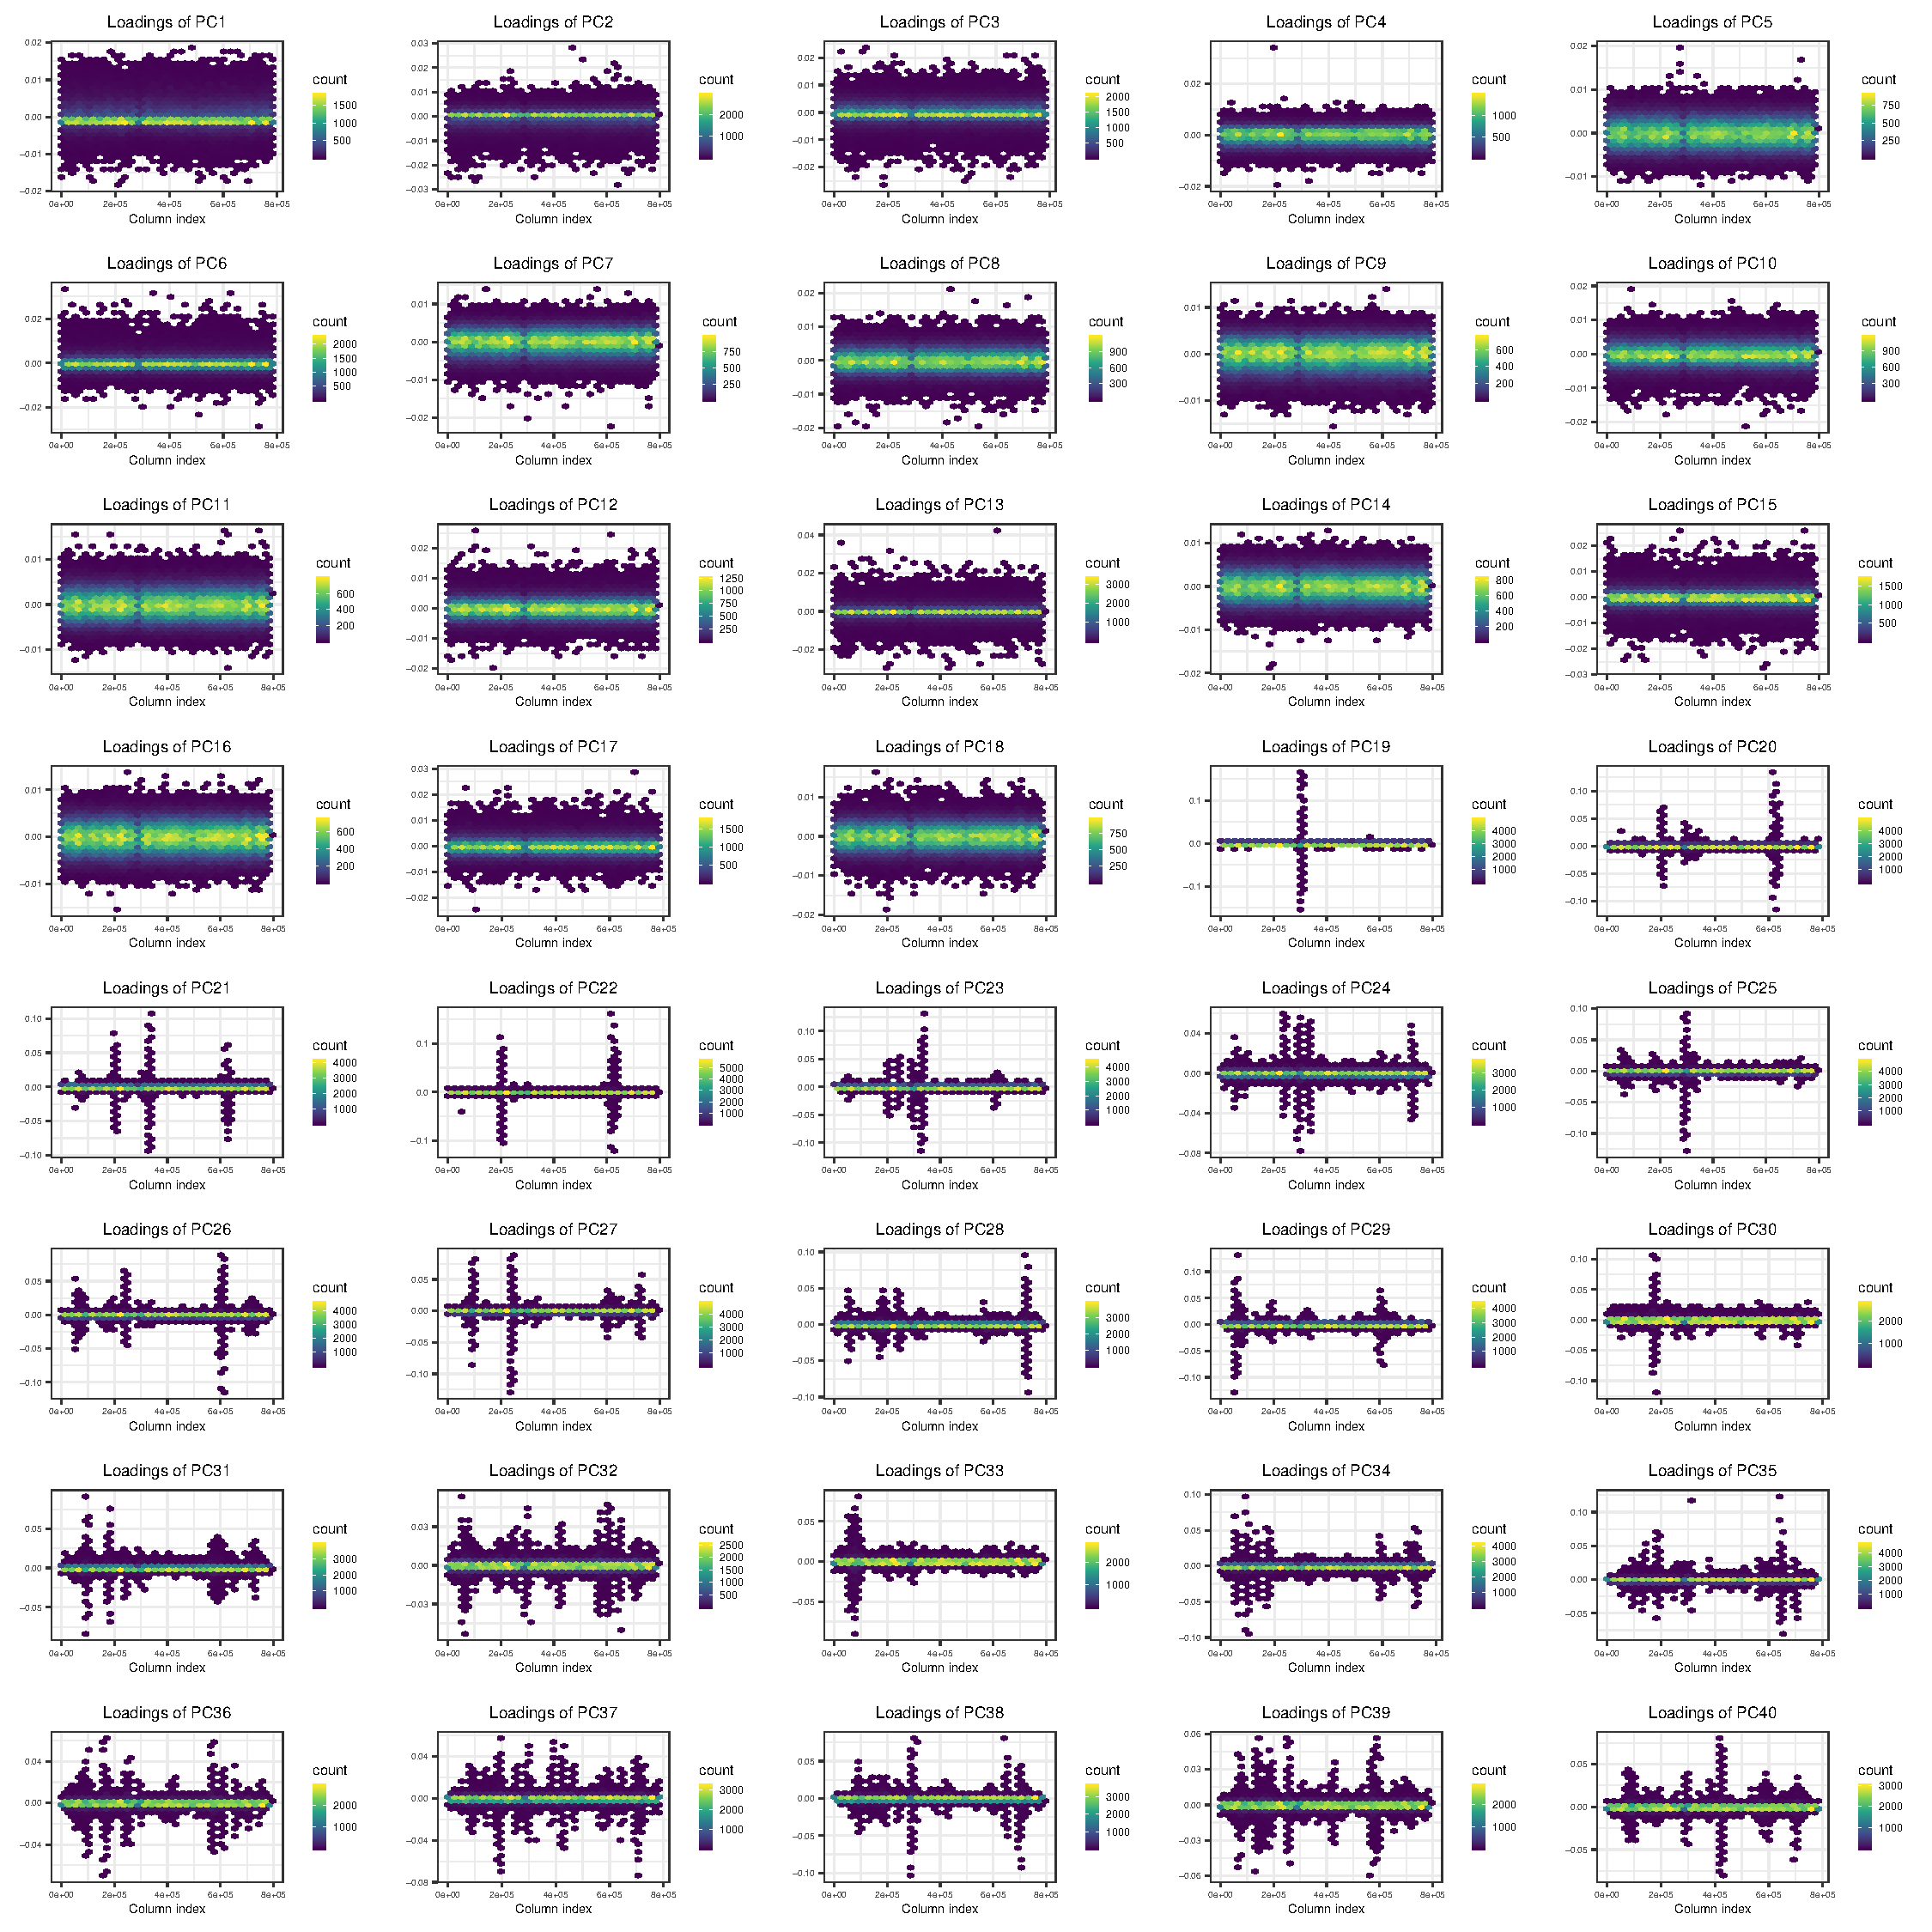
\includegraphics[width=0.9\textwidth]{UKBB-loadings1-40.pdf}}
\caption{Principal Component (PC) loadings 1 to 40 reported by the UK Biobank.
\label{fig:UKBB-loadings40}}
\end{figure}

As for other analyses, it takes 8 minutes to match the 1000G data to the UKBB data and compute 20 PCs of the 1000G data using the automatic LD detection technique. It takes 12 minutes more to do the OADP projection of all 488,371 individuals of the UKBB data onto the PCA computed using the 1000G data.
Finally, it takes only 6 minutes to compute the 30-Nearest Neighbours of 20 PC scores for 406,545 UK Biobank individuals, which is the main computational aspect of computing the statistics used to detect individual outlier samples (Section \ref{outlier-sample}).

\subsection{Outlier sample detection}

To detect a few sample outliers, we compare the standard rule of ``6 SDs from the mean'' (6SD) used in e.g.\ EIGENSOFT to the statistic we propose in section \ref{outlier-sample}.
Our statistic identifies only isolated samples or isolated pairs that seems to be outliers driving structure of PC17-20 of 1000G (Figure \ref{fig:outlier-pd}).
In contrast, 6SD identifies a lot of outliers, of which some are part of a relatively large cluster (Figure \ref{fig:outlier-sd}).
We recall that, in theory, if all PCs are normally distributed, after correcting for multiple testing of 2500 individuals and 20 PCs, 6SD has a small probability of 0.0001 of detecting one outlier or more.

\begin{figure}[htbp]
\centering
\begin{subfigure}[b]{0.5\textwidth}
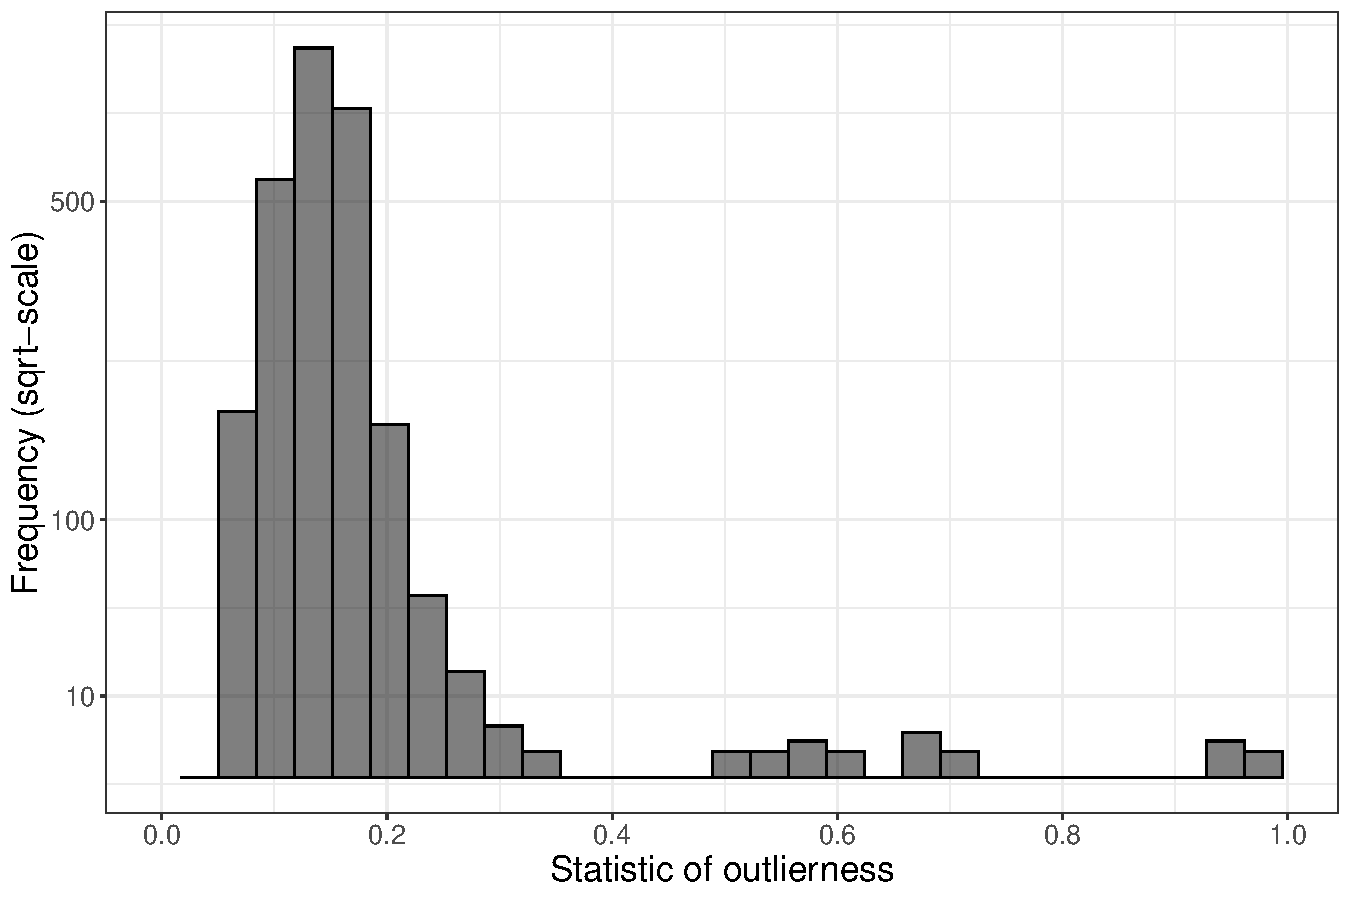
\includegraphics[width=\textwidth]{hist-outliers-1000G.pdf}
\caption{Distribution of statistics}
\end{subfigure}
\\~\\
\begin{subfigure}[b]{0.45\textwidth}
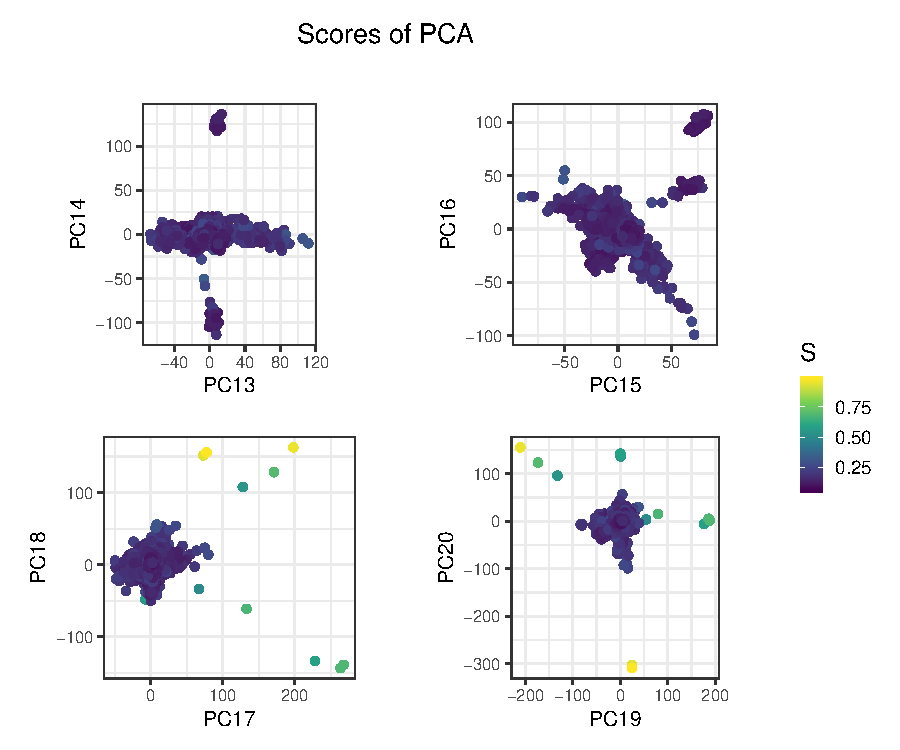
\includegraphics[width=\textwidth]{outliers-1000G.pdf}
\caption{Principal Component (PC) scores 13 to 20 of 1000G, colored by the statistic (S) used to define outliers.\\~\\}
\end{subfigure}
~~~~~~
\begin{subfigure}[b]{0.45\textwidth}
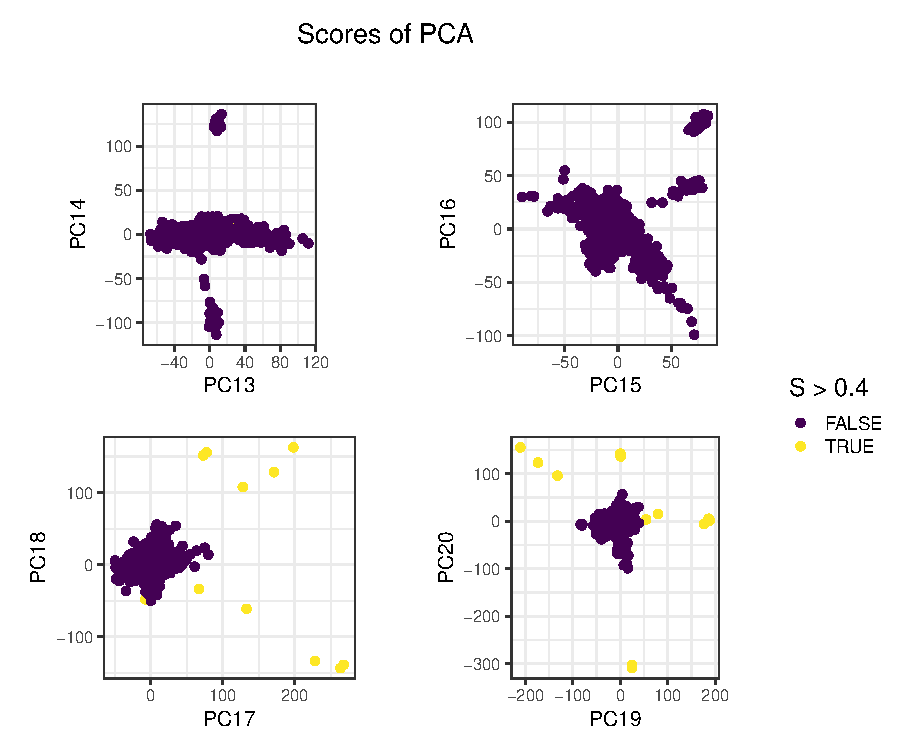
\includegraphics[width=\textwidth]{be-outlier-1000G.pdf}
\caption{Principal Component (PC) scores 13 to 20 of 1000G, colored by being detected as an outlier. Threshold of being an outlier is determined based on histogram (a).}
\end{subfigure}
\caption{Outlier detection in the 1000 Genomes (1000G) project, using \texttt{prob\_dist} (Section \ref{outlier-sample}).\label{fig:outlier-pd}}
\end{figure}

When the goal is to restrict to homogeneous samples, we compare the use of R package aberrant used to report the ``White British'' subset of UKBB homogeneous samples, to the use of the robust Mahalanobis distance we propose.
Here, we visually choose a threshold of 5 on the log-distance and show that this gives a similar subset of individuals than the ``White British'' subset reported by the UK Biobank (Figure \ref{fig:homogeneous}).
Moreover, when using this threshold, only 3 out of 10,936 people of Asian ancestry (1 ``Chinese'' and 2 ``Indian'') are kept, and 1 ``African'' out of 7622 poeple with Black background is kept (Table \ref{tab:homogeneous}). 
In contrast, 416,492 out of 431,090 ``British'' (96.6\%) and 12,620 out of 12,759 ``Irish'' (98.9\%) are kept.

\subsection{Projecting PCs from a reference dataset}

We use 60\% of individuals in the 1000G data (section \ref{1000G}) to compute K=20 PCs. Then, we project the remaining 40\% individuals using three methods: 1/ simply multiplying the genotypes of these individuals by the previously computed loadings, 2/ correcting the simple projections using asymptotic shrinkage factors as determined by R package hdpca v1.1.3 \cite[]{dey2019asymptotic}, with all eigenvalues derived from the Genetic Relationship Matrix (GRM) computed with new function \texttt{bed\_tcrossprodSelf} of R package bigsnpr, and 3/ the OADP projection (section \ref{proj}). 
When simply projecting using loadings, there is negligible shrinkage for PC1 and PC2, a small shrinkage for PC3 and PC4, and a large shrinkage for PC5 to PC8 (Figure \ref{fig:proj1000G}).
In contrast, there is no visible shrinkage when projecting new individuals with OADP (Figure \ref{fig:proj1000G}).
Simple projection is affected even more by this shrinkage for PC9 to PC20, while OADP still appears free of this issue (Figure \ref{fig:proj1000G-2}).
We show the same results when projecting the full UK Biobank data onto PCA computed using 1000G data  (Figure \ref{fig:proj1000G-5}).
When correcting projected PC scores with asymptotic shrinkage factors, bias is smaller than when simply projecting loadings, yet, there is a visible bias for PC7-8 (Figure \ref{fig:proj1000G-3}).
Finally, to assess if OADP could be used to project individuals that are related to some individuals that were used to compute PCA, we projected these 60\% individuals (as if we were projecting their monozygotic twins) using OADP. Projections of related individuals using OADP shows some bias in reverse direction (Figure \ref{fig:proj1000G-4}).
\label{proj-related}

\begin{figure}[!htpb]
\centerline{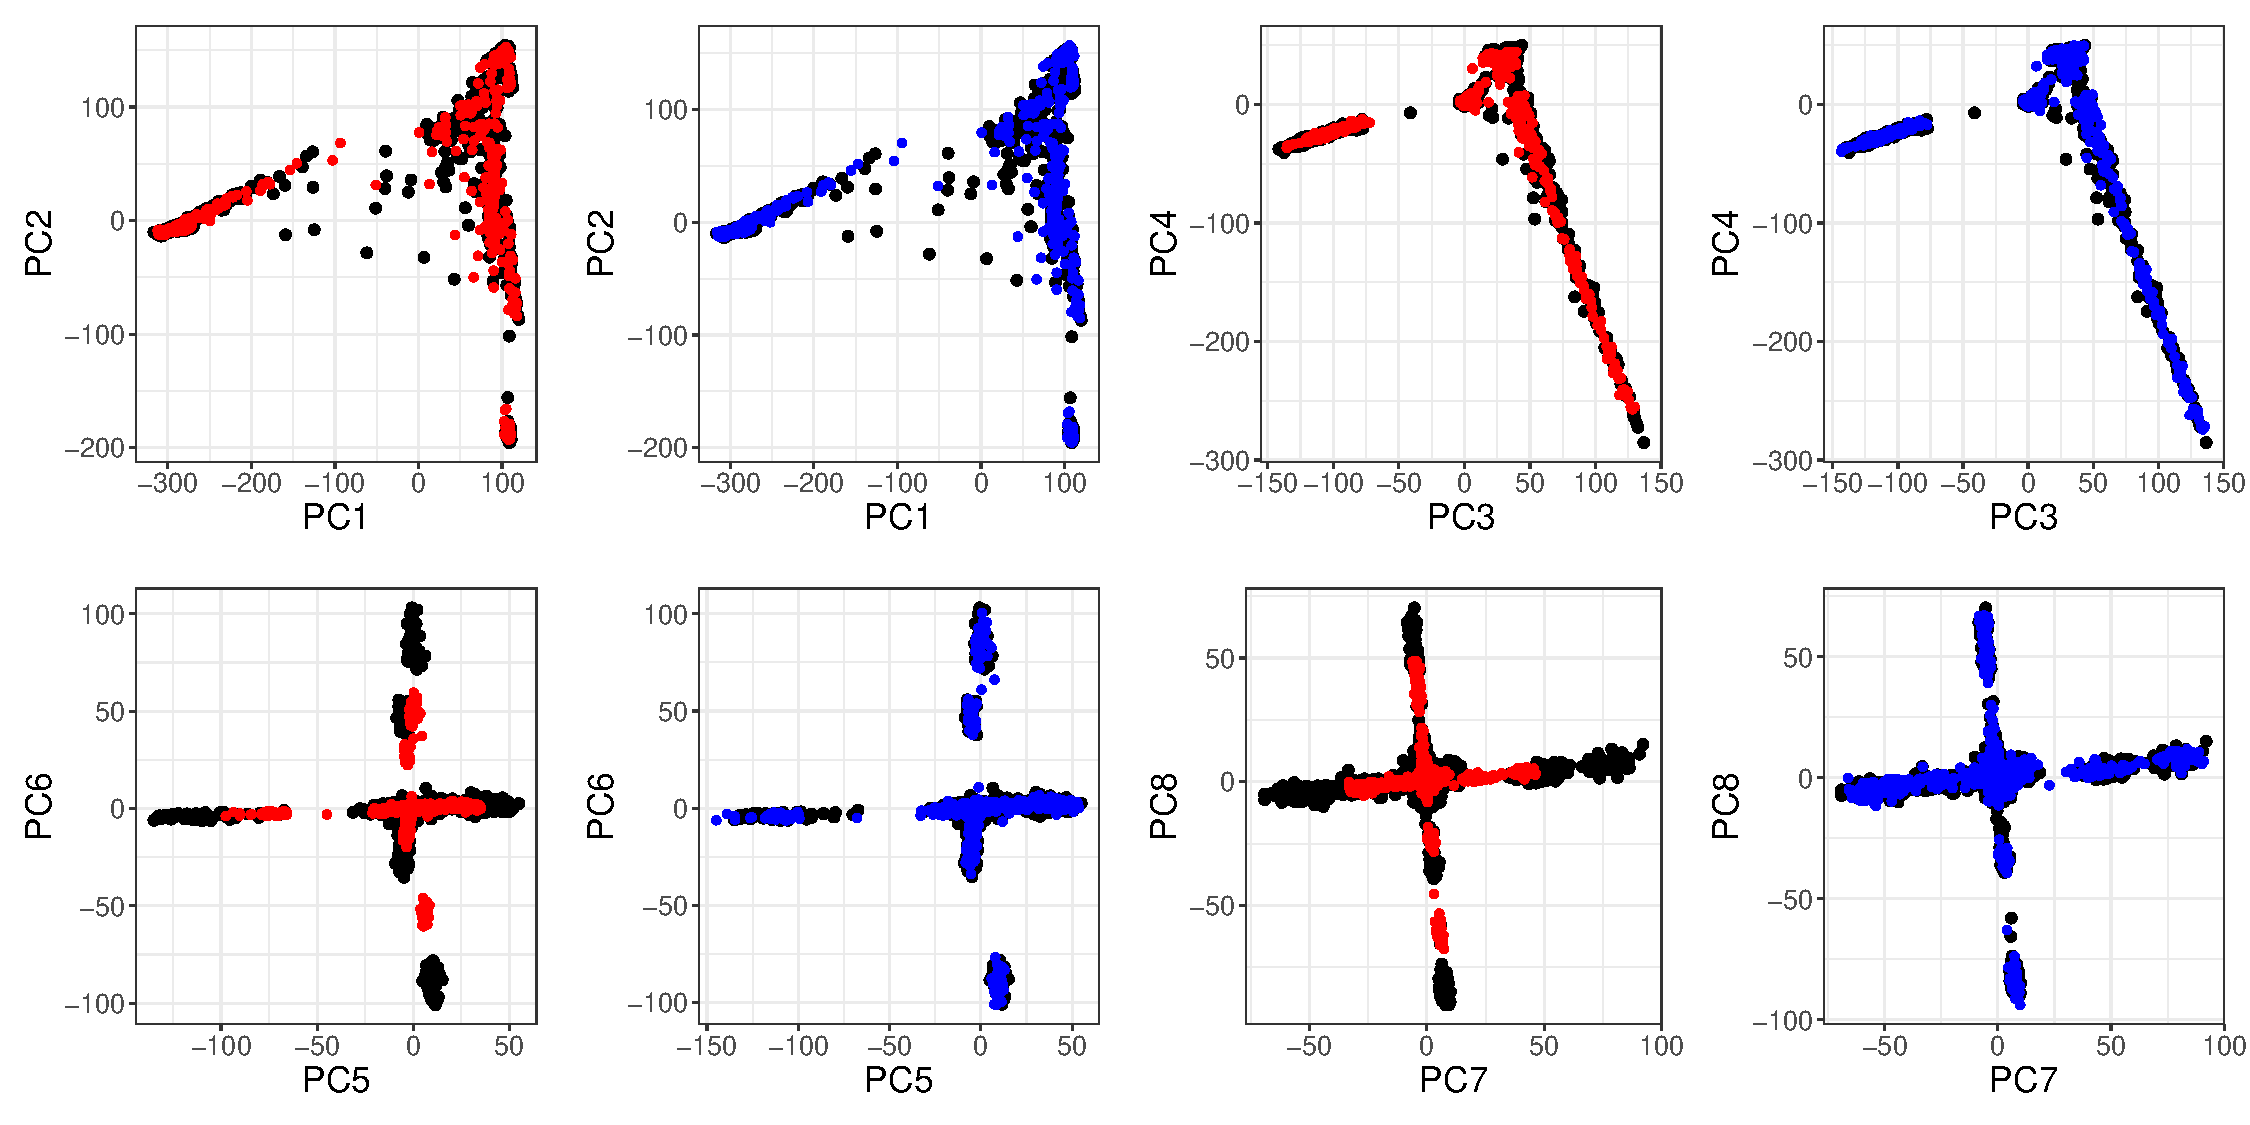
\includegraphics[width=0.8\textwidth]{proj1000G-PC1-8.pdf}}
\caption{Principal Component (PC) scores 1 to 8 of the 1000 Genomes project.
Black points are the 60\% individuals used for computing PCA.
Red points are the 40\% remaining individuals, projected by simply multiplying their genotypes by the corresponding PC loadings.
Blue points are the 40\% remaining individuals, projected using the Online Augmentation, Decomposition, and Procrustes (OADP) transformation.
Estimated shrinkage coefficients for these 8 PCs are 1.01 (PC1), 1.02, 1.06, 1.09, 1.50 (PC5), 1.69, 1.98 and 1.39.
\label{fig:proj1000G}}
\end{figure}

When computing the PCs on the UK Biobank using 406,545 unrelated individuals and 171,977 variants, and projecting the 1000G data onto this reference PCA space, shrinkage is much smaller ($\leq 1.08$ for all 20 first PCs, Figure \ref{fig:proj1000G-6}). Overall, shrinkage decreases with an increased sample size (Table \ref{tab:shrinkage}).

\begingroup
\renewcommand*{\arraystretch}{1.8}
\begin{table}[h]
\centering
\caption{Shrinkage coefficients when projecting new individuals onto reference PCA space. We list the dataset, the sample size and number of variants used to compute the final PCA. As expected, the shrinkage bias only becomes negligible if the PCA is conducted on large samples.} 
\label{tab:shrinkage}
\begin{tabular}{|c|c|c|c|}
\hline
Dataset & Sample size ($\times$1000) & \makecell {Number of variants \\ ($\times$1000, after LD removal)} & Shrinkage (PC 1 - 5 - 10 - 20) \\
\hline
1000G & ~~~~1.5 & 393 & 1.01 - 1.50 - 3.14 - 6.70 \\
1000G & ~~~~2.5 & 229 & 1.01 - 1.36 - 2.84 - 6.75 \\
UKBB & ~~49.0 & 282 & 1.00 - 1.04 - 1.12 - 1.43 \\
UKBB & 406.5 & 172 & 1.00 - 1.01 - 1.04 - 1.08 \\
\hline
\end{tabular}
\end{table}
\endgroup


\subsection{Capturing subtle population structure in the UK Biobank}

We recomputed PCA in the UK Biobank after restricting the individuals included in the computations: we randomly subsampled UKBB data to use only 10,000 British individuals (out of 431,029) and 5000 Irish individuals (out of 12,755), while keeping all individuals with other or unknown self-reported ancestry. 
We further removed all pairs of related individuals reported by the UKBB (i.e.\ both individuals in each pair). 
This resulted in 48,942 individuals that we used to compute 50 PCs, which took less than 3 hours using function \texttt{bed\_autoSVD} (that converged after 4 iterations of automatic LD removal). 
We show that we are able to capture more PCs (at least 40 instead of 16-18) that display visual population structure (Figures \ref{fig:UKBB-scores2} and \ref{fig:UKBB-screeplot2}).
We then projected all 439,429 remaining individuals from UKBB onto this PCA space in 21 minutes only using our implementation of the OADP projection (\texttt{bed\_projectSelfPCA}). Note that these individuals should not be related to any of the 48,942 individuals used for training PCA because we removed both individuals from each pair of related individuals in UKBB. Projection of new individuals show again a clear shrinkage when using simple projection (between 1.00 for PC1 and 1.80 for PC50), but no visible bias when using OADP projection (Figure \ref{fig:projUKBB-related}).

\begin{figure}[!htpb]
\centerline{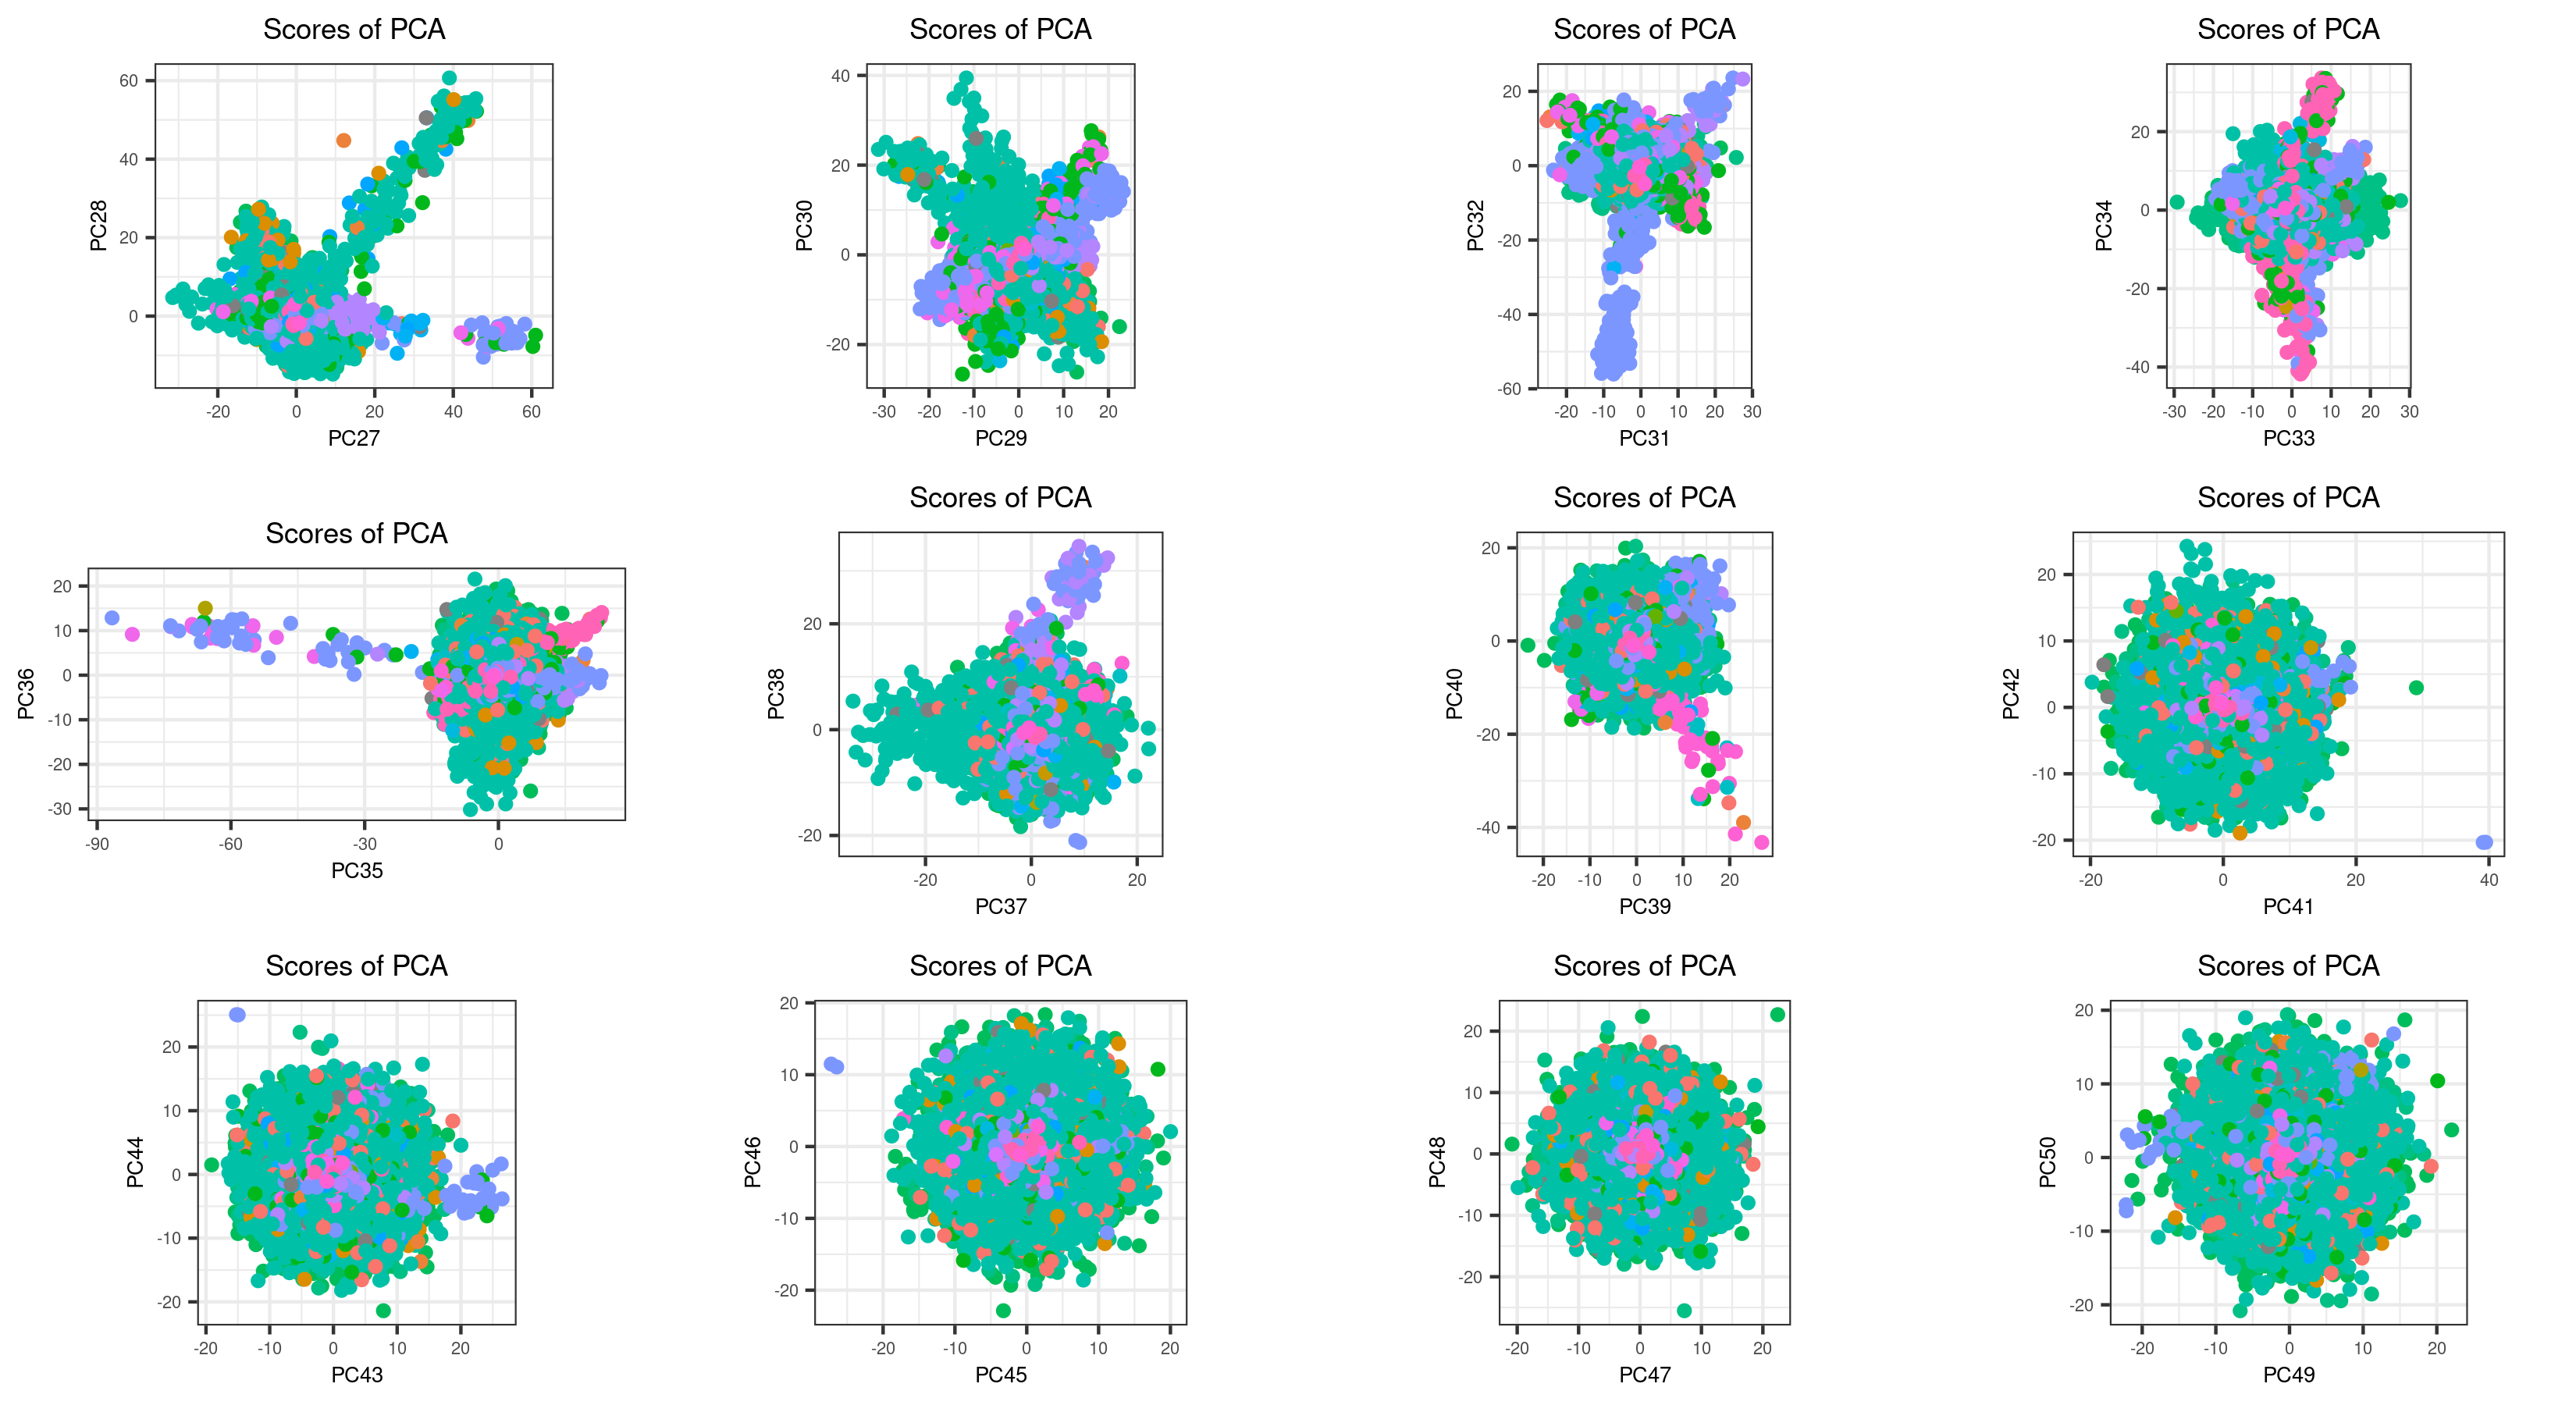
\includegraphics[width=0.9\textwidth]{UKBB-scores-restricted.png}}
\caption{Principal Component (PC) scores 27 to 50 computed on the UK Biobank using 48,942 individuals of diverse ancestries. These individuals are the ones resulting from removing all related individuals and randomly subsampling the British and Irish individuals. Different colors represent different self-reported ancestries.
\label{fig:UKBB-scores2}}
\end{figure}

%%%%%%%%%%%%%%%%%%%%%%%%%%%%%%%%%%%%%%%%%%%%%%%%%%%%%%%%%%%%%%%%%%%%%%%%%%%%%%%%

\section{Discussion}

\begin{figure}[!htpb]
\centerline{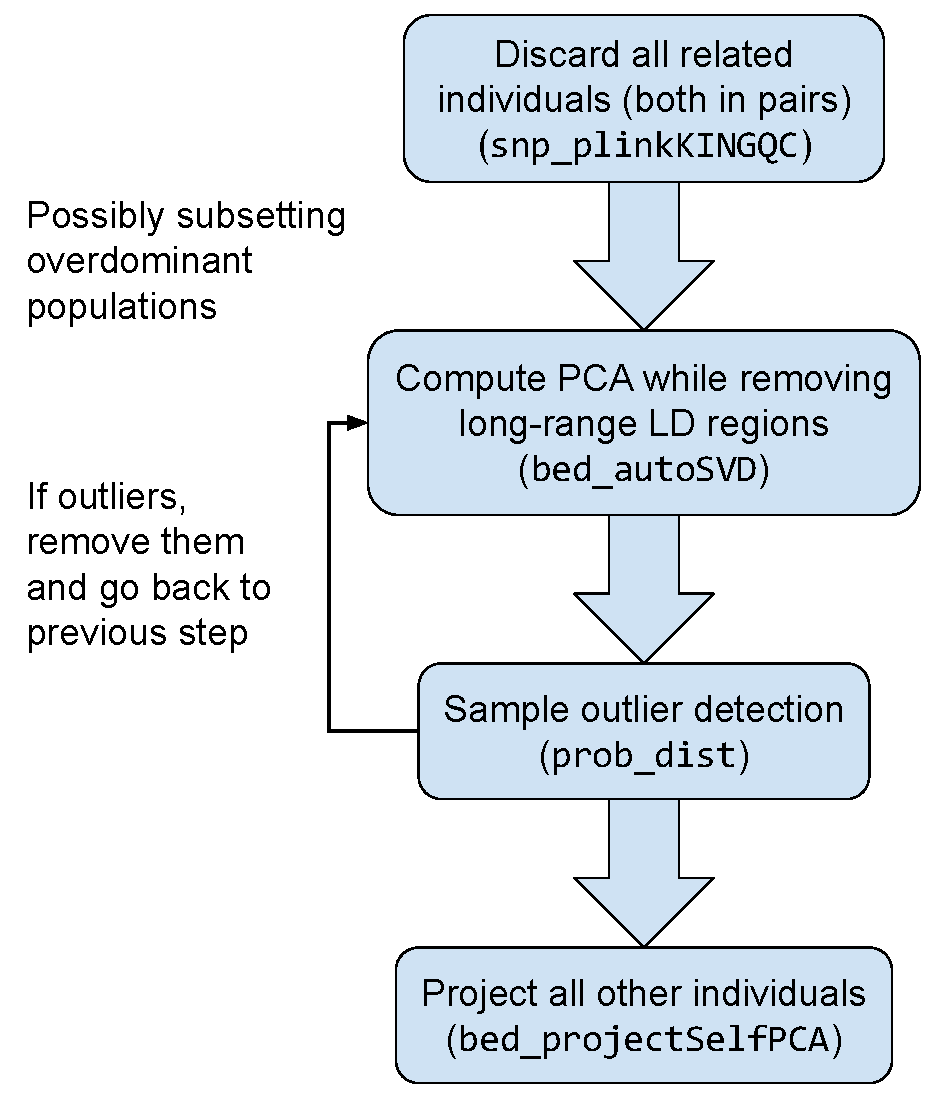
\includegraphics[width=0.4\textwidth]{PCA-pipeline.pdf}}
\caption{Pipeline for computing Principal Components (PCs) using R packages bigsnpr and bigutilsr.
\label{fig:pipeline}}
\end{figure}

In this work, we have compiled different pitfalls that can arise with analyses related to Principal Component Analysis (PCA) of genetic data. Then, we have investigated possible solutions to these pitfalls and chose the ones that we found most relevant, both with respect to properties such as accuracy and robustness, but also that would be fast and easy to use. We then implemented these solutions in open-source R packages. 
The new functions we provide can be directly applied to genotypes stored as PLINK bed/bim/fam files with some missing values.
This contrasts with previous releases of package bigsnpr that could only use one custom data format called ``bigSNP''. This data format can store both genotype calls and dosages, but requires conversion from other formats and imputation of missing values using functions provided in the package \cite[]{prive2017efficient}.
As PCA is a useful tool on its own and does not require extensive imputed data, we therefore decided that operating directly on PLINK files with a few missing values would be more practical for users.

As a general recommendation for computing PCA, we propose the pipeline shown in figure \ref{fig:pipeline}. Note that we have not included standard steps such as initial quality control filters and post-analysis checks (e.g.\ visual inspection of different plots).
This pipeline requires removing all related individuals, for which we provide an R wrapper to PLINK's implementation of KING robust kinship coefficients \cite[]{manichaikul2010robust,chang2015second}. 
Note that one should remove both individuals in each related pairs so that the projected individuals are not related to the ones used for computing PCA, as we showed that relatedness is a problem when using the OADP projection (Figure \ref{fig:proj1000G-4}).
After selecting a subset of individuals, we apply several steps of outlier detection, one for outlier variants that capture long-range LD variation (automatic), and one for detecting outlier samples (semi-automatic and visual).
To make these steps more computationally efficient, we explored solutions for not recomputing PCA from scratch when removing a few samples or variants. Using educated guesses in R package PRIMME based on low-rank approximations seemed to be a promising approach but did not reduce computation time by much, so we did not pursue this idea \cite[]{brand2003fast,wu2017primme}. 
Once PCA is done, one should look at the loadings to make sure that there is no visible LD structure left (peaks in PC loadings as shown in figures \ref{fig:UKBB-loadings40} and \ref{fig:UKBB-loadings}), since including PCs that capture LD as covariates in genetic analyses can lead to reduced power for variants in these regions. 
These long-range LD regions are captured by PCs because variants in these regions are extensively correlated (even after a first step of LD thinning), and PCA just captures the variance in these correlated variants. 
This is a similar problem as including related individuals or even whole families in PCA, they would show up as structure in PCs. 
One should also look at PC scores to identify which PCs capture population structure.
As in many applications, we believe there should be a compromise between signal and noise. Therefore, we recommend using only PCs that show structure (e.g.\ PC1-16 in figure \ref{fig:UKBB-scores}) and exclude PCs that indicate LD (e.g.\ PC19-40 in figure \ref{fig:UKBB-loadings40}).

We also provide some recommendations when the dataset is composed mainly of one population (e.g.\ British people in the UK Biobank).
We show that it is useful to actually subset these individuals so there is not too much imbalance between the sample sizes of the different populations. Previous work has also shown that uneven population sizes can distort PCs \cite[]{novembre2008interpreting,mcvean2009genealogical}. 
Indeed, when subsetting British and Irish people, we are able to capture a lot more PCs that show population structure with less than 50K individuals as compared to when using more than 400K unrelated individuals.
This makes designs such as the 1000 Genomes project, which gathered around 100 people for each of 26 populations, highly relevant for capturing population structure.
In contrast, when the goal is to have an homogeneous sample, we show that using the Mahalanobis distance on PC scores can efficiently achieve this goal, which we used in previous analyses \cite[]{prive2019efficient}.
When the homogeneous sample is not predominant in the dataset, one solution is to compute the center and covariance of the robust Mahalanobis distance using only the population of interest, and then computing the distances for all individuals using these robust estimates. 

Finally, although we have focused on PCA of genotype data in this paper, we believe most of the results presented here are not inherent to genotype data, and can be transferred to e.g.\ other omics data as well. For example, PCs can be used to account for confounding in other data as well \cite[]{pickrell2010understanding}. Then, outlier and homogeneous sample detection can be used on PCs of other types of data. Moreover, projection of scores will also be a problem for other omics data where the number of variables used is larger than the number of samples used for computing PCA. Finally, using ``populations'' with approximately the same size is relevant for other biological data as well.
However, other pitfalls might apply when using other types of data; for example, methylation data can be confounded by factors such as age and sex, and it might be benificial to remove some probes that are associated with these confounding factors before computing PCA \cite[]{decamps2019guidelines}.

%%%%%%%%%%%%%%%%%%%%%%%%%%%%%%%%%%%%%%%%%%%%%%%%%%%%%%%%%%%%%%%%%%%%%%%%%%%%%%%%

\newpage

\section*{Software and code availability}

All code used for the analyses of this paper is available at \url{https://github.com/privefl/paper4-bedpca/tree/master/code}.

Package bigsnpr can be installed from GitHub (see \url{https://github.com/privefl/bigsnpr}).

A tutorial on the steps to perform PCA on 1000G data is available at \url{} [TODO]. 

\section*{Acknowledgements}

Authors thank Rounak Dey and Seunggeun Lee for helpful discussions about PCA projection.
This research has been conducted using the UK Biobank Resource under Application Number 25589.

F.P., J.M.\ and B.V.\ are supported by the Danish National Research Foundation (Niels Bohr Professorship to J.M.), and also acknowledge the Lundbeck Foundation Initiative for Integrative Psychiatric Research, iPSYCH (R248-2017-2003).

\section*{Declaraction of Interests}

Michael Blum is now an employee of OWKIN France.
The other authors declare no competing interests.

%%%%%%%%%%%%%%%%%%%%%%%%%%%%%%%%%%%%%%%%%%%%%%%%%%%%%%%%%%%%%%%%%%%%%%%%%%%%%%%%

\newpage

\bibliographystyle{natbib}
\bibliography{refs}

%%%%%%%%%%%%%%%%%%%%%%%%%%%%%%%%%%%%%%%%%%%%%%%%%%%%%%%%%%%%%%%%%%%%%%%%%%%%%%%%

\newpage
\section*{Supplementary Materials}

\renewcommand{\thefigure}{S\arabic{figure}}
\setcounter{figure}{0}
\renewcommand{\thetable}{S\arabic{table}}
\setcounter{table}{0}

\subsection*{Optimised OADP transformation}

We implement an optimised version of the Online Augmentation, Decomposition, and Procrustes (OADP) transformation when using $K''=K'=K$ \cite[]{zhang2019fast}.
We assume that the $K$-partial Singular Value Decomposition (SVD) of the reference matrix $X$ (of size $n \times p$) has been computed as $U \Delta V^T$. There are several steps to perform OADP transformation for each sample $y$ (of size $1 \times p$) of target matrix $Y$ (of size $m \times p$):
\begin{enumerate}
\item Calculate $l = y \cdot V$ (of size $1 \times K$), where $V$ are the K PC loadings. And $g = y \cdot h^T$ (of size $1 \times 1$), where $h = (y - l \cdot V^T) / ||y - l \cdot V^T||_2$. Actually, $||y - l \cdot V^T||_2^2 = y \cdot y^T - 2 \cdot y \cdot V \cdot l^T  + l \cdot V^T \cdot V \cdot l^T = y \cdot y^T - l \cdot l^T$ and $y \cdot (y - l \cdot V^T)^T = y \cdot y^T - y \cdot V \cdot l^T = y \cdot y^T - l \cdot l^T$. Then $g = \sqrt{y \cdot y^T - l \cdot l^T}$.
\item Calculate $Q^T Q$ where $$Q = \begin{bmatrix} \Delta & l^T \\ 0 & g \end{bmatrix}$$ so that $$Q^TQ = \begin{bmatrix} \Delta^2 & \Delta \cdot l^T \\ l \cdot \Delta & g^2 + l \cdot l^T \end{bmatrix} = \begin{bmatrix} \Delta^2 & \Delta \cdot l^T \\ l \cdot \Delta & y \cdot y^T \end{bmatrix}.$$ Note that we do not actually need to compute $g$, and that we can update only the last row and column of $Q^T Q$ instead of computing it from an updated version of $Q$.
\item Get the eigen decomposition $Q^T Q = V' {\Delta'}^2 {V'}^T$ (truncated to $K$ components out of the $K+1$). Let us denote $V_2 = V' {\Delta'}$.
\item Calculate $$\begin{bmatrix} \widetilde{U} \\ \widetilde{u}  \end{bmatrix} = \begin{bmatrix} U & 0 \\ 0 & 1 \end{bmatrix} V_2 = \begin{bmatrix} U V_2[1{:}K,~] \\ V_2[K{+}1,~] \end{bmatrix} $$
\item Find the Procrustes transformation from $\widetilde{U}$ to $U \Delta$. As $\widetilde{U}$ and $U \Delta$ have both their columns centered already (since $U$ does), the Procrustes transformation $\rho \widetilde{U} A$, where $\rho$ is a scaling coefficient and $A$ is an orthonomal projection matrix that minimise the Frobenius norm of $(\rho \widetilde{U} A - U)$, is given by $A = V'' {U''}^T$ and $\rho = \frac{\text{trace}(\Delta'')}{\text{trace}(\widetilde{U}^T \widetilde{U})}$ where $U'' \Delta'' {V''}^T$ is the full SVD of $(U \Delta)^T \widetilde{U}$ \cite[]{wang2015improved}. 
As $U^T U = I$, we note that $(U \Delta)^T \widetilde{U} = \Delta V_2[1{:}K,~]$ and that $\rho = \frac{\text{trace}(\Delta'')}{\text{trace}({V_2[1{:}K,~]}^T V_2[1{:}K,~])}$, therefore we do not need to explicitly compute $\widetilde{U}$ and do not need $U$. 
\item Apply the previous transformation to $\widetilde{u}$ to get the projection of $y$ in the reference PCA space (i.e.\ $\rho \widetilde{u} A$).
\end{enumerate}


%%%%%%%%%%%%%%%%%%%%%%%%%%%%%%%%%%%%%%%%%%%%%%%%%%%%%%%%%%%%%%%%%%%%%%%%%%%%%%%%

\clearpage

\subsection*{Supplementary figures}

%%%%%%%%%%%%%%%%%%%%%%%%%%%%%%%%%%%%%%%%%%%%%%%%%%%%%%%%%%%%%%%%%%%%%%%%%%%%%%%%

\begin{figure}[htbp]
\centering
\begin{subfigure}[b]{0.5\textwidth}
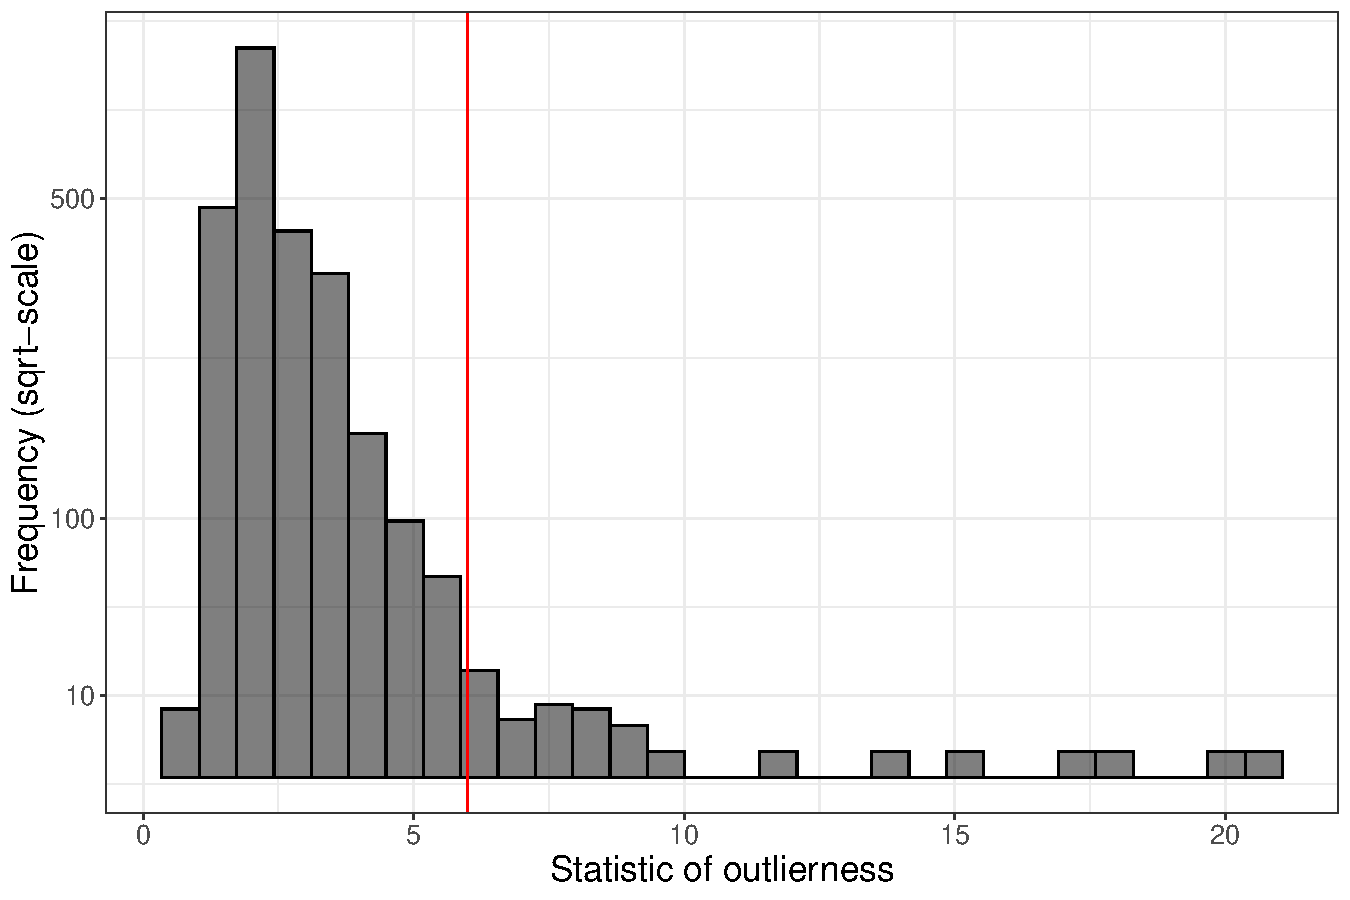
\includegraphics[width=\textwidth]{hist-outliers2-1000G.pdf}
\caption{Distribution of statistics and default threshold (6, in red)}
\end{subfigure}
\\~\\
\begin{subfigure}[b]{0.45\textwidth}
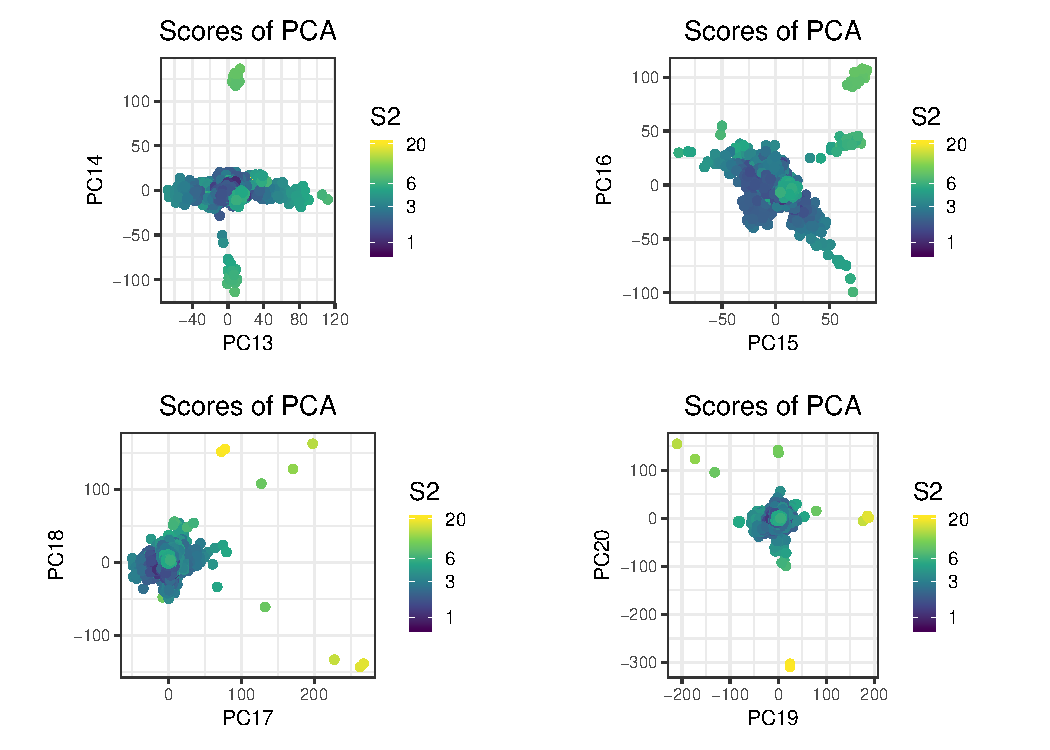
\includegraphics[width=\textwidth]{outliers2-1000G.pdf}
\caption{Principal Component (PC) scores 13 to 20 of 1000G, colored by statistic used to detect outliers (maximum number of SDs from the mean, log-scale).}
\end{subfigure}
~~~~~~
\begin{subfigure}[b]{0.45\textwidth}
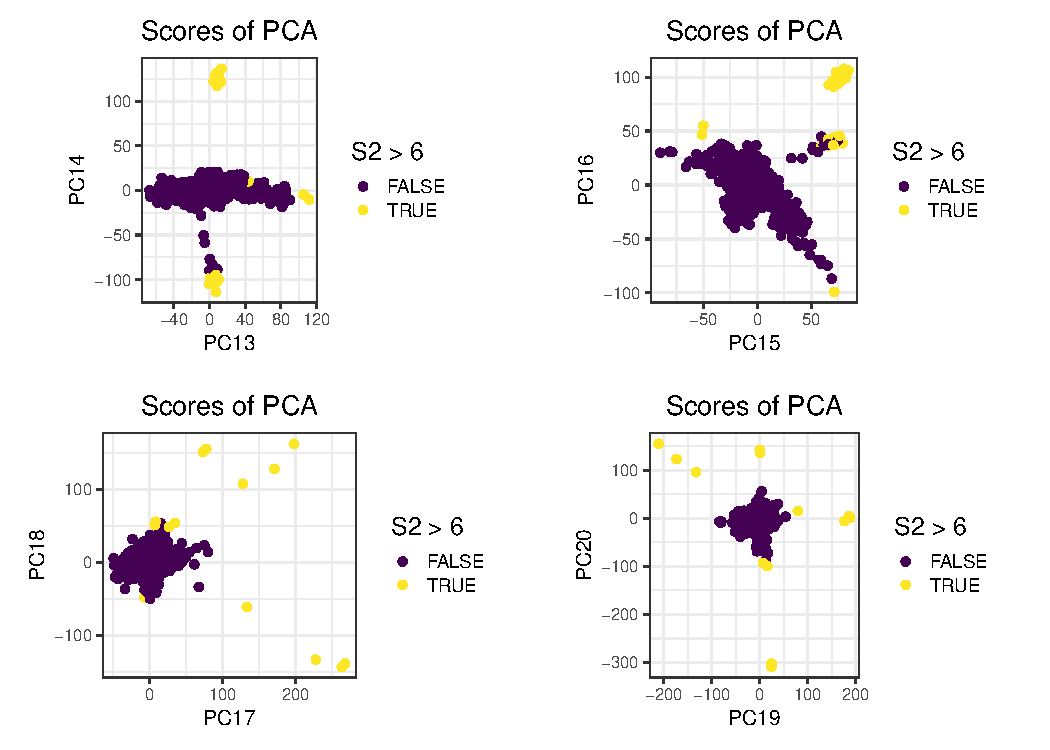
\includegraphics[width=\textwidth]{be-outlier2-1000G.pdf}
\caption{Principal Component (PC) scores 13 to 20 of 1000G, colored by being detected as an outlier.\\}
\end{subfigure}
\caption{Outlier detection in the 1000 Genomes (1000G) project, using the rule ``6 SDs from the mean'', i.e.\ where S2 is the maximum (for all PCs) number of SDs from the mean (Section \ref{outlier-sample}).\label{fig:outlier-sd}}
\end{figure}

%%%%%%%%%%%%%%%%%%%%%%%%%%%%%%%%%%%%%%%%%%%%%%%%%%%%%%%%%%%%%%%%%%%%%%%%%%%%%%%%

\newpage

\begin{figure}[htbp]
\centering
\begin{subfigure}[b]{0.45\textwidth}
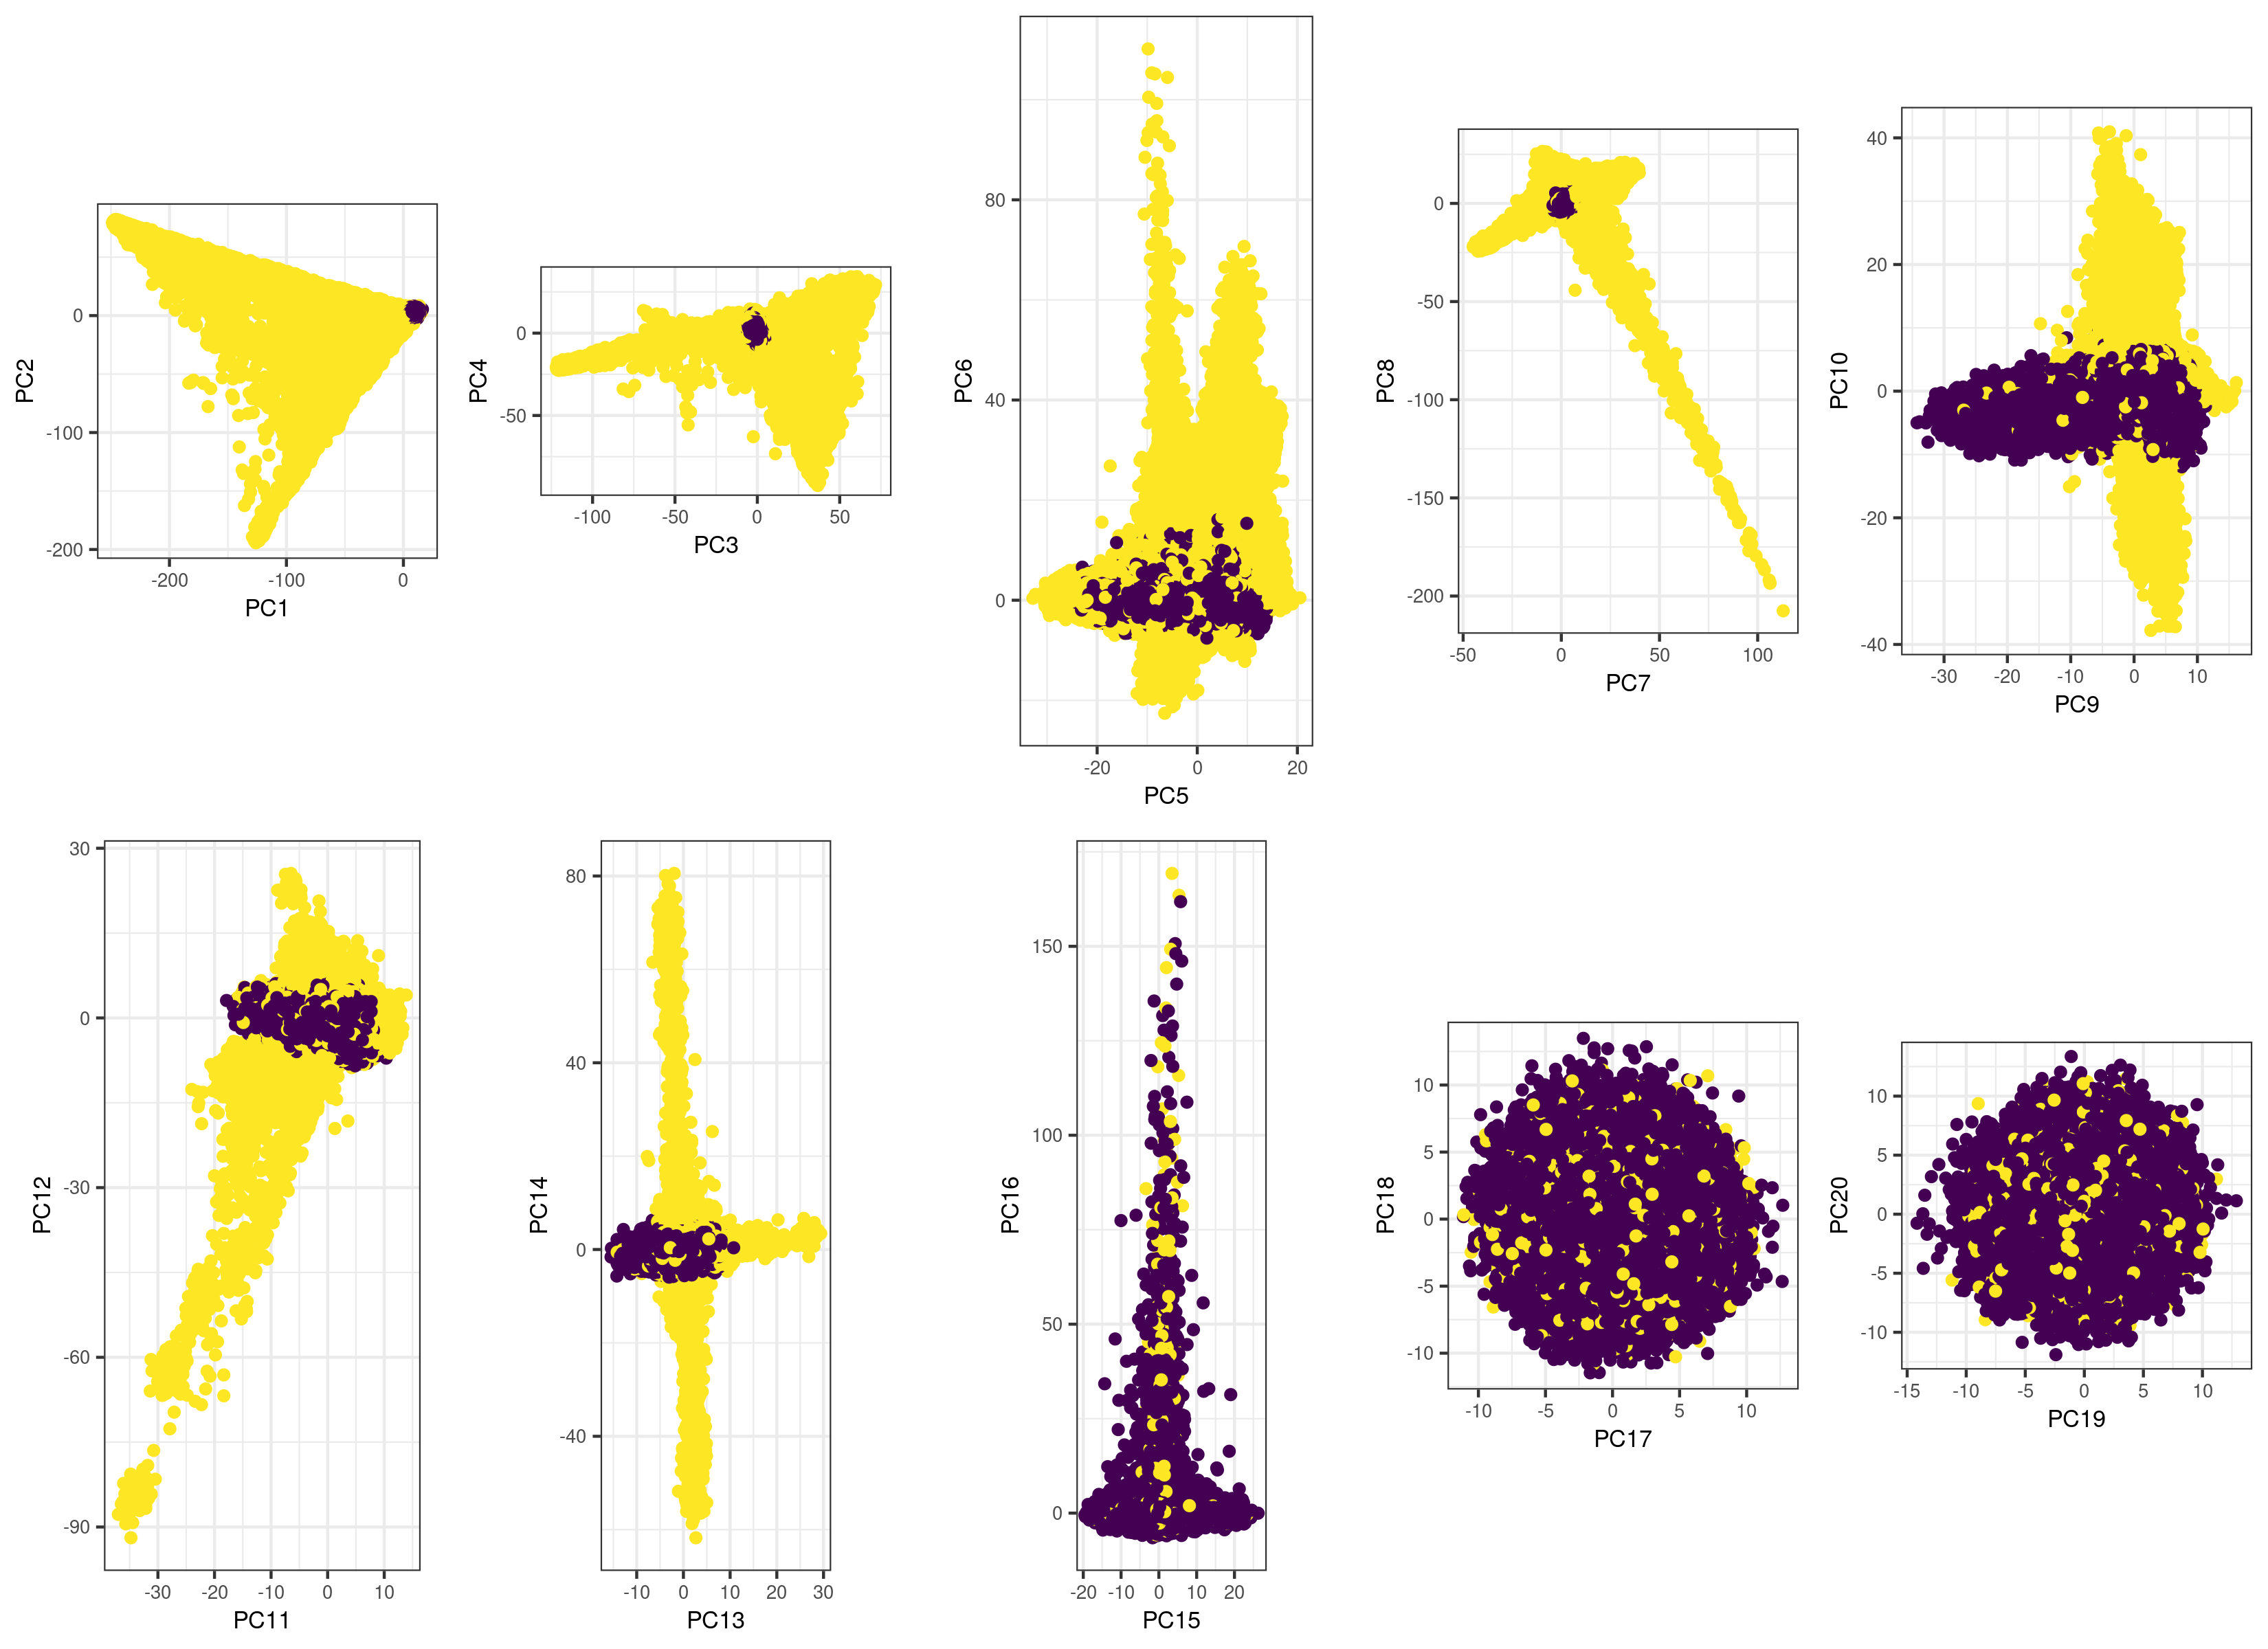
\includegraphics[width=\textwidth]{UKBB-White-British.png}
\caption{PCs 1 to 20 of UKBB, colored by whether it is in the group of ``White British'' reported by the UKBB (blue).}
\end{subfigure}
~~~~~~
\begin{subfigure}[b]{0.5\textwidth}
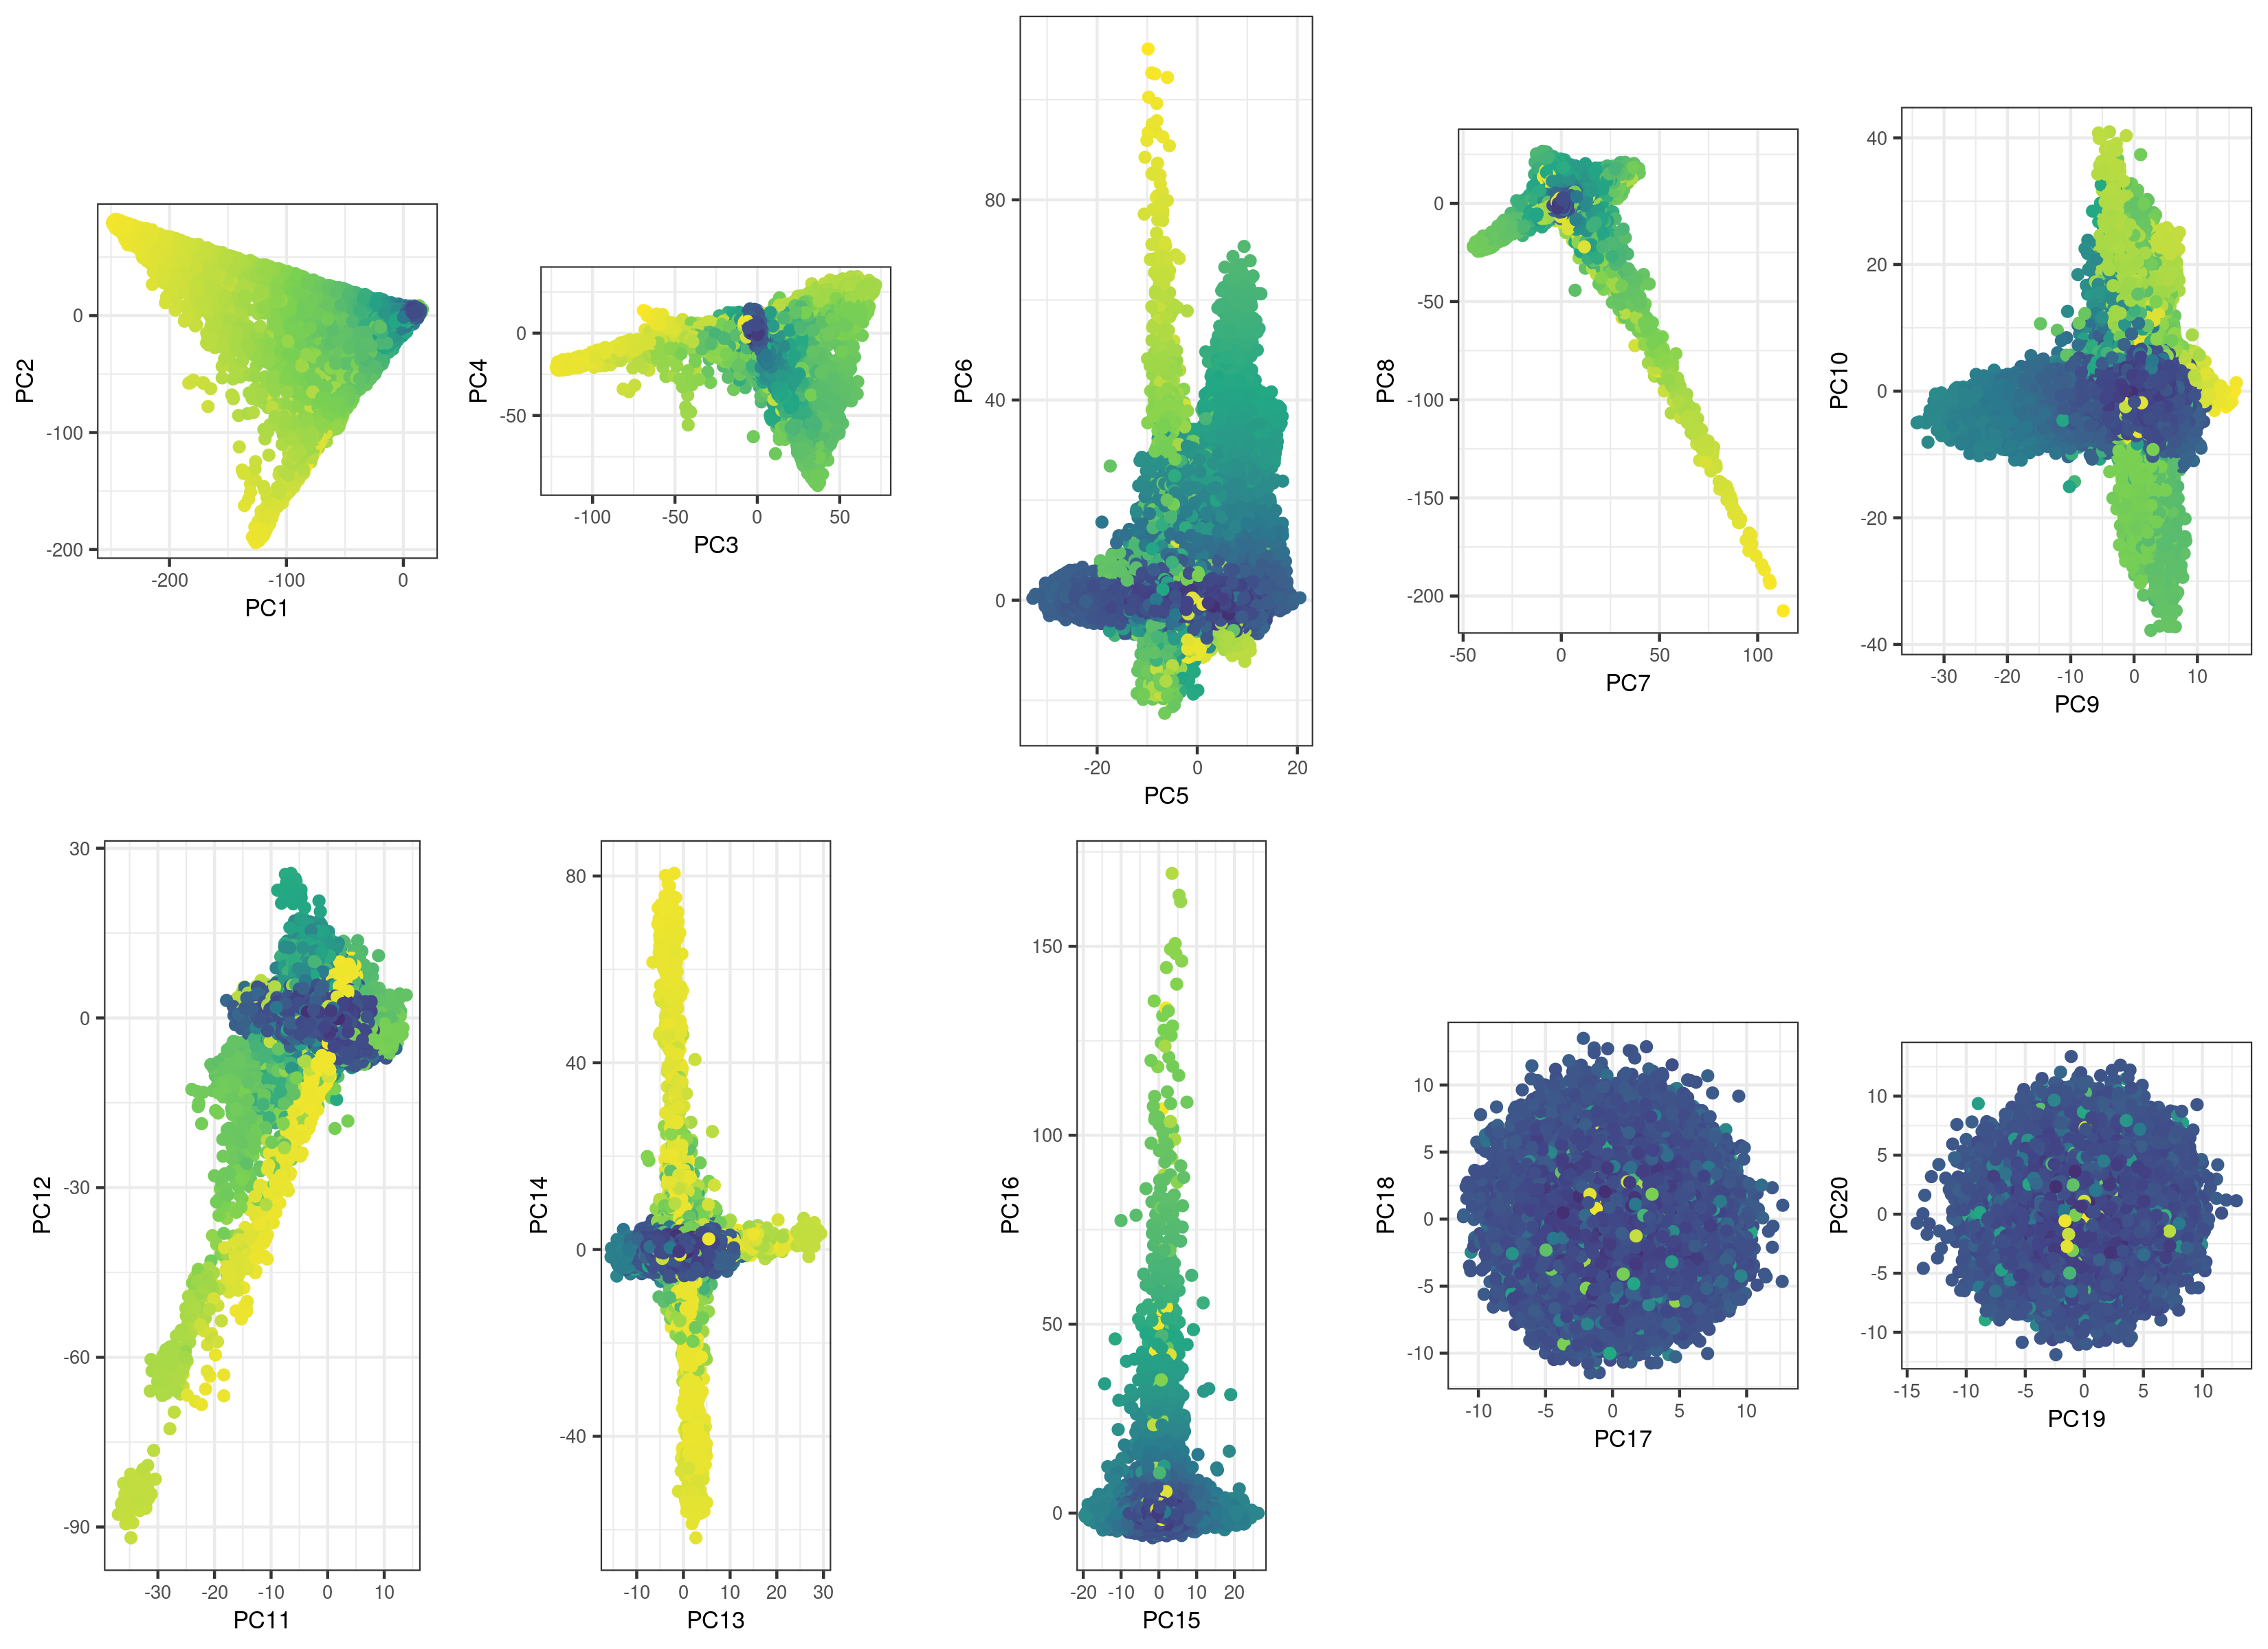
\includegraphics[width=\textwidth]{UKBB-Maha-dist.png}
\caption{PCs 1 to 20 of UKBB, colored by robust Mahalanobis distances computed on PCs (log-scale).\\}
\end{subfigure}
\\~\\
\begin{subfigure}[b]{0.45\textwidth}
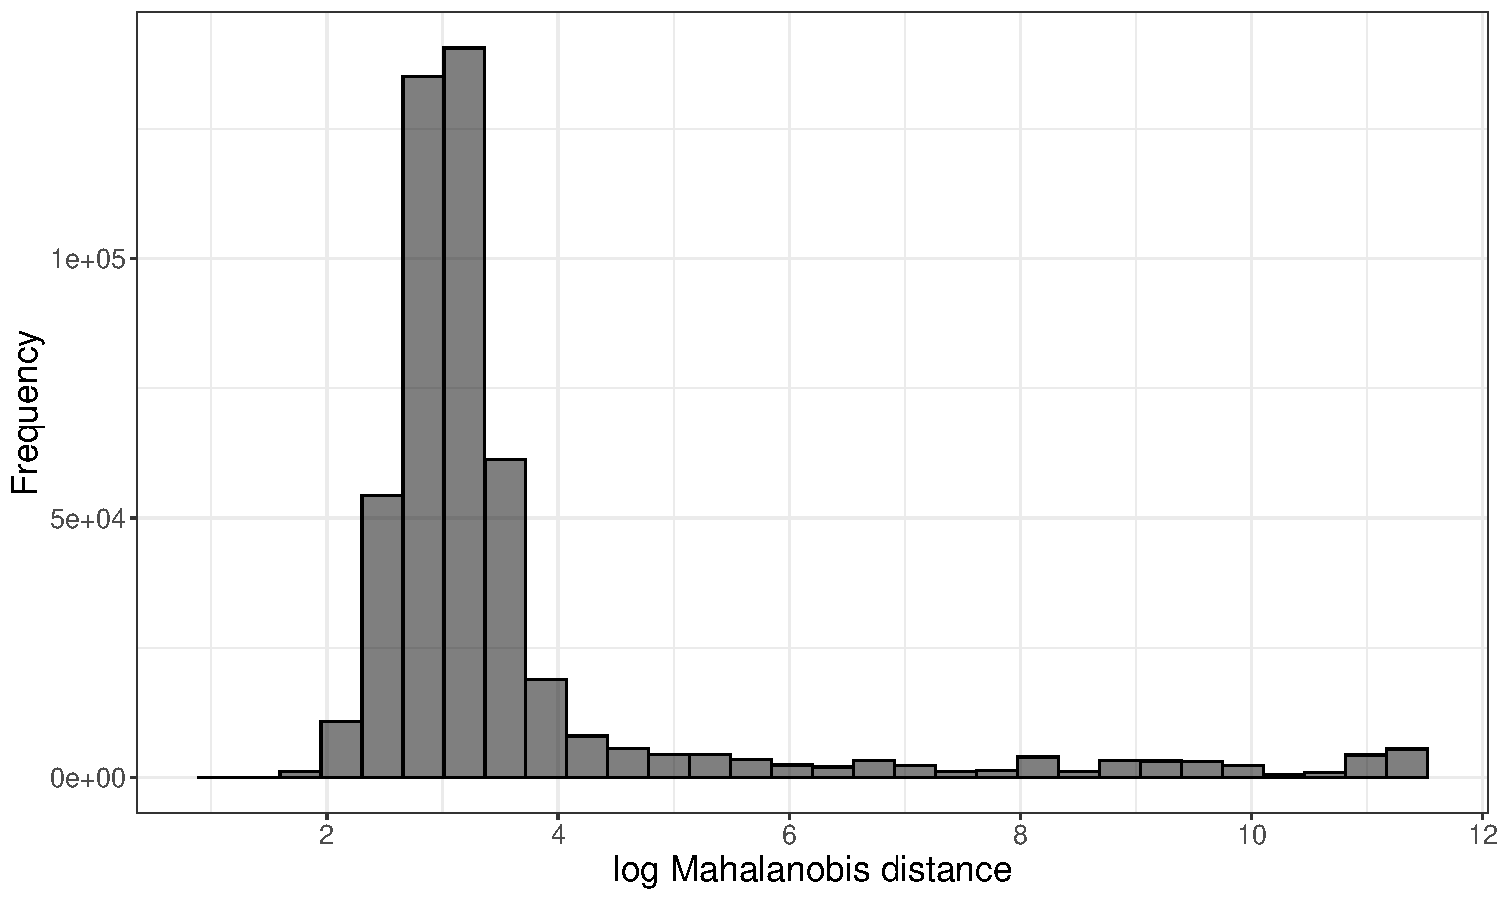
\includegraphics[width=\textwidth]{hist-Maha-dist.pdf}
\caption{Distribution of (log squared) distances.\\~\\~\\~\\~\\}
\end{subfigure}
~~~~~~
\begin{subfigure}[b]{0.45\textwidth}
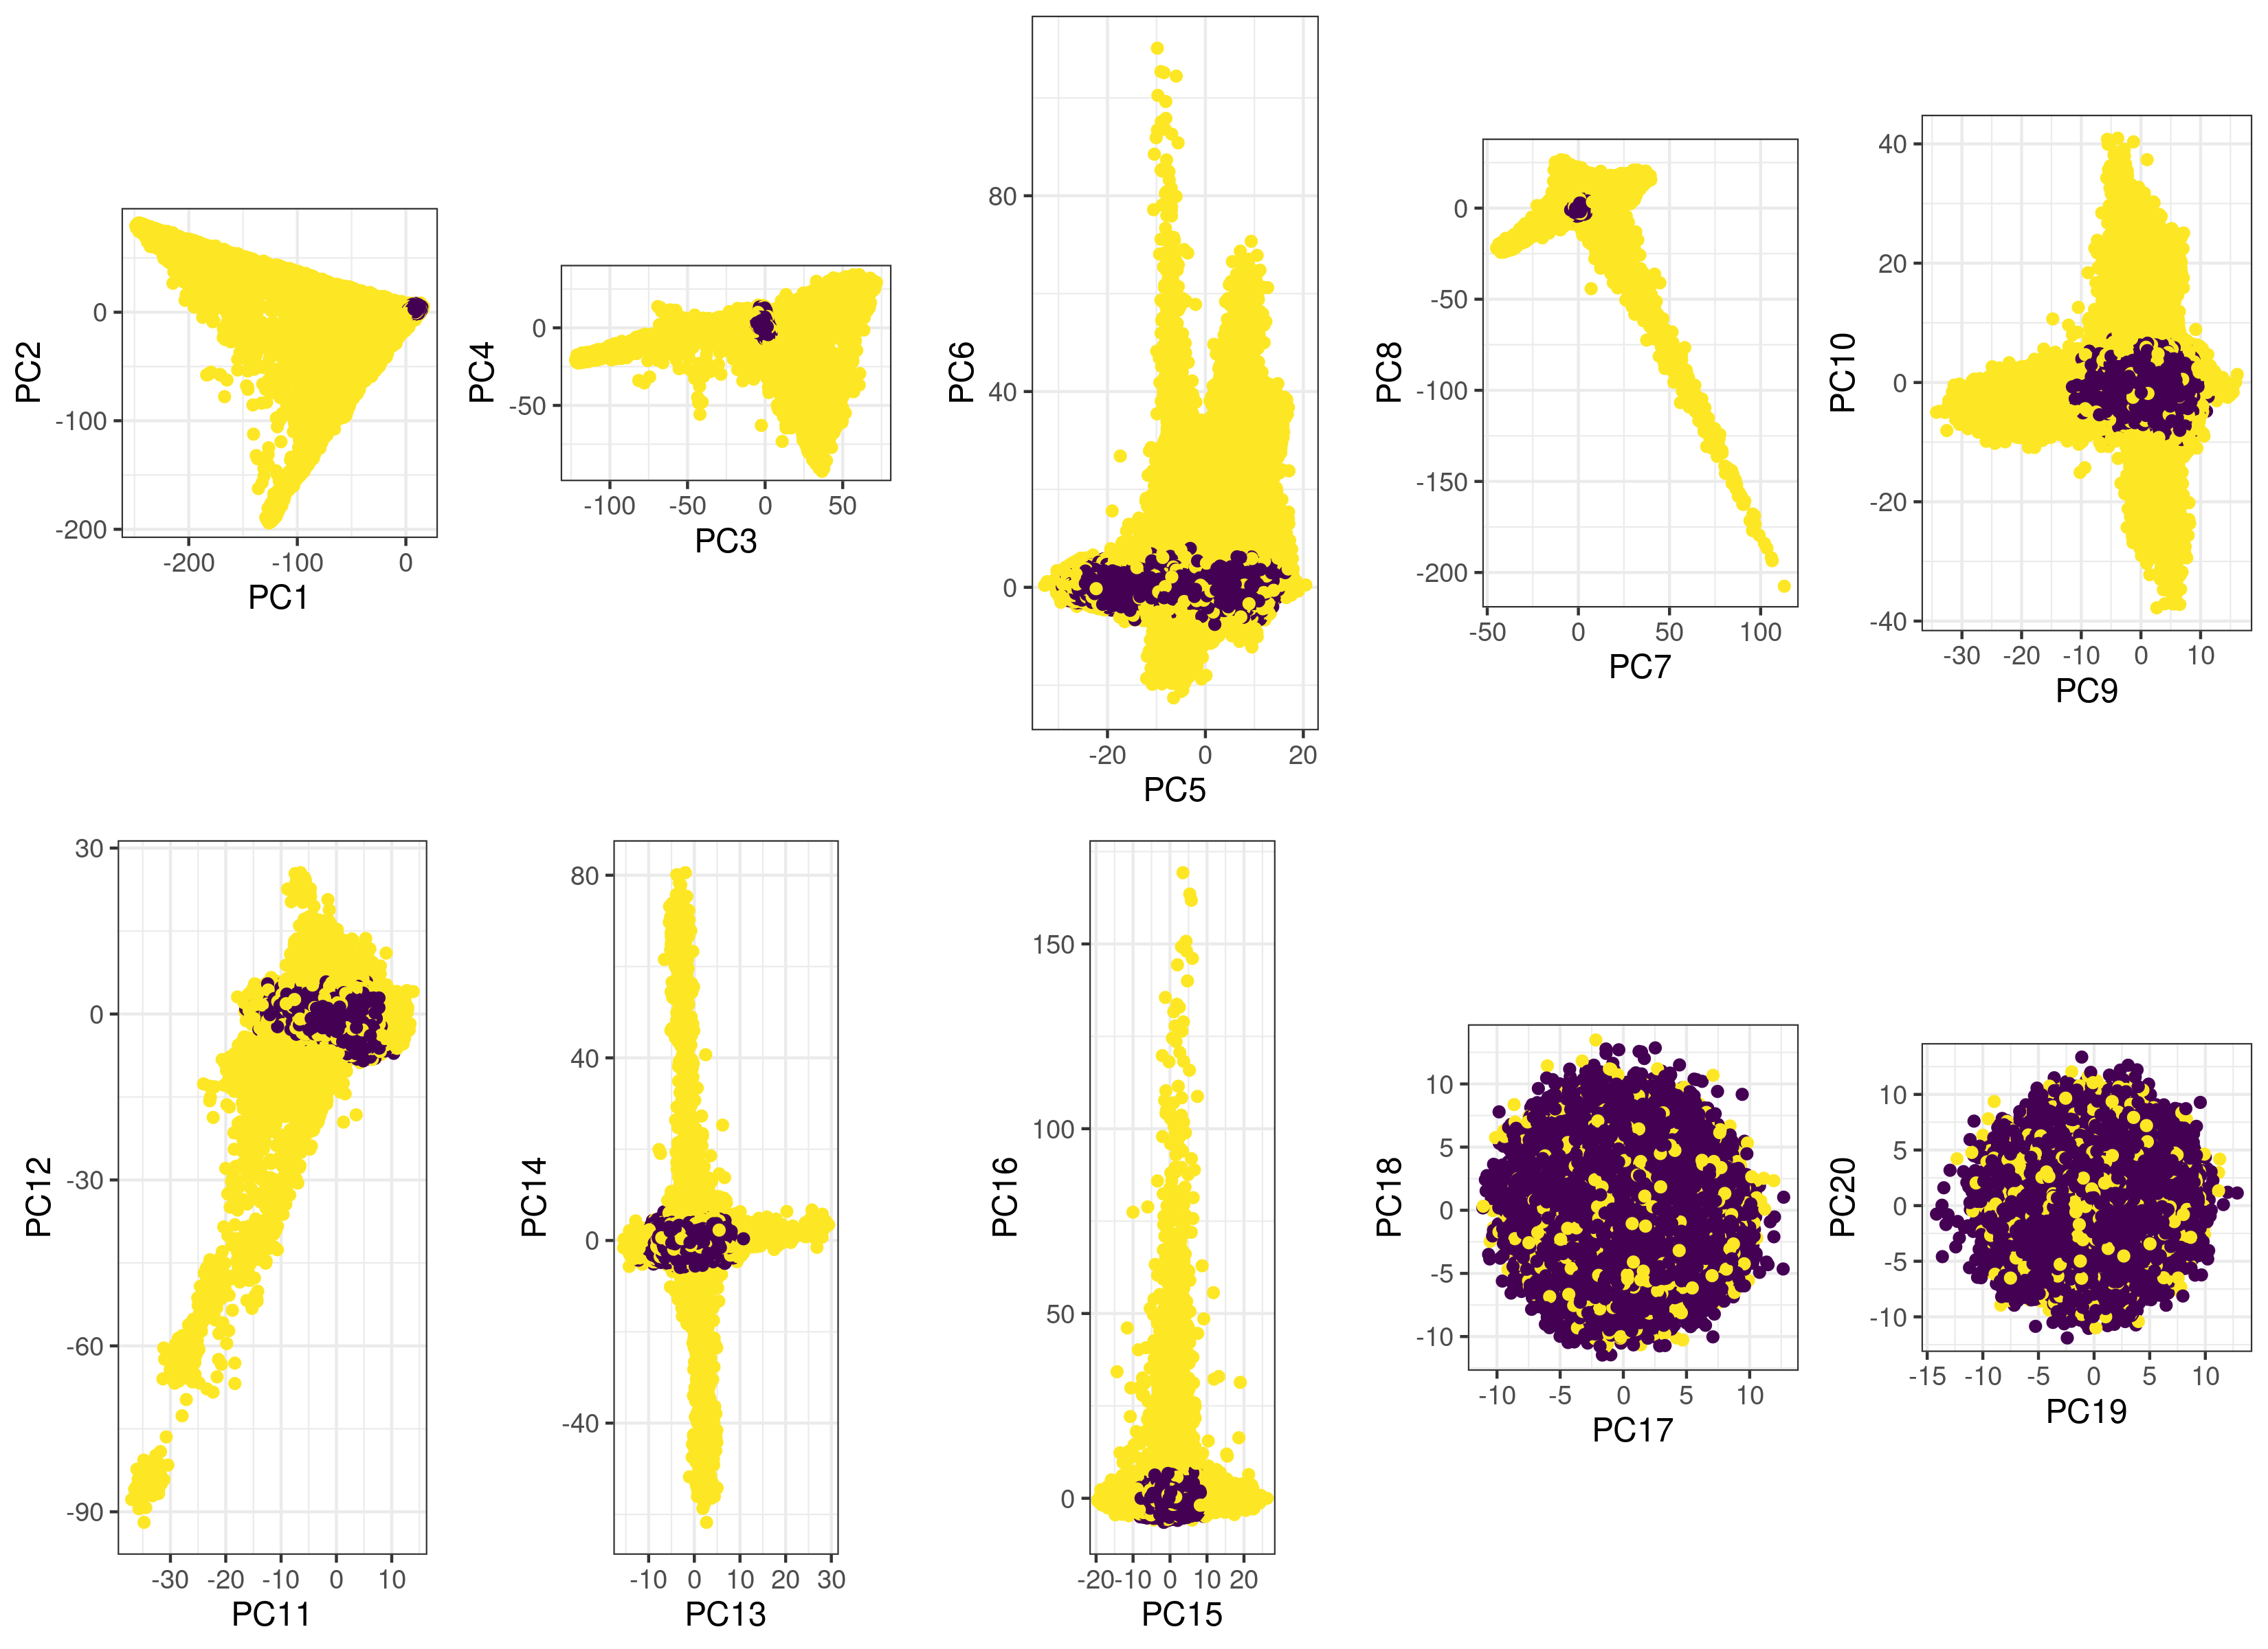
\includegraphics[width=\textwidth]{UKBB-Maha-outlier.png}
\caption{PCs 1 to 20 of UKBB, colored by being detected as an outlier. Threshold of being considered as an outlier is determined based on histogram (c), where the threshold of 5 is chosen for the logarithm of the distances.}
\end{subfigure}
\caption{Homogeneous sample detection in the UK Biobank (UKBB), using robust Mahalanobis distances computed on the first 20 Principal Component scores (PCs) of UKBB.).\label{fig:homogeneous}}
\end{figure}

% latex table generated in R 3.6.0 by xtable 1.8-4 package
% Sat Nov  9 10:17:25 2019
\begin{table}[ht]
\centering
\caption{Number of UKBB individuals with (log squared) Mahalanobis distance lower than some threshold (top), and grouped by self-reported ancestry (left). Note that ``$<$ 12'' includes all individuals.} 
\label{tab:homogeneous}
\begin{tabular}{|l|r|r|r|r|r|r|r|r|r|r|}
  \hline
 & $<$ 3 & $<$ 4 & $<$ 5 & $<$ 6 & $<$ 7 & $<$ 8 & $<$ 9 & $<$ 10 & $<$ 11 & $<$ 12 \\ 
  \hline
Prefer not to answer & 484 & 1013 & 1062 & 1099 & 1139 & 1177 & 1279 & 1405 & 1471 & 1583 \\ 
  Do not know & 36 & 68 & 76 & 84 & 92 & 118 & 155 & 188 & 196 & 204 \\ 
  White & 186 & 422 & 457 & 483 & 513 & 533 & 543 & 543 & 545 & 546 \\ 
  Mixed & 2 & 6 & 6 & 7 & 8 & 15 & 26 & 42 & 46 & 46 \\ 
  Asian or Asian British &  &  &  &  &  & 3 & 20 & 40 & 42 & 42 \\ 
  Black or Black British & 1 & 2 & 2 & 2 & 2 & 2 & 2 & 4 & 6 & 26 \\ 
  Chinese &  & 1 & 1 & 1 & 1 & 2 & 5 & 21 & 1423 & 1504 \\ 
  Other ethnic group & 57 & 230 & 261 & 314 & 469 & 885 & 1939 & 2761 & 3681 & 4356 \\ 
  British & 191713 & 400516 & 416492 & 424490 & 427769 & 429172 & 431026 & 431082 & 431089 & 431090 \\ 
  Irish & 1416 & 12039 & 12620 & 12700 & 12734 & 12743 & 12759 & 12759 & 12759 & 12759 \\ 
  Any other white background & 1468 & 4747 & 6953 & 9341 & 12979 & 14613 & 15741 & 15810 & 15820 & 15820 \\ 
  White and Black Caribbean & 1 & 4 & 4 & 4 & 9 & 35 & 142 & 537 & 589 & 597 \\ 
  White and Black African & 1 & 3 & 3 & 4 & 6 & 29 & 99 & 333 & 400 & 402 \\ 
  White and Asian & 4 & 7 & 13 & 23 & 79 & 350 & 651 & 790 & 802 & 802 \\ 
  Any other mixed background & 24 & 66 & 87 & 155 & 274 & 391 & 595 & 884 & 990 & 996 \\ 
  Indian &  & 2 & 2 & 5 & 6 & 29 & 1682 & 5700 & 5716 & 5716 \\ 
  Pakistani &  &  &  &  & 1 & 13 & 532 & 1747 & 1748 & 1748 \\ 
  Bangladeshi &  &  &  &  &  &  & 2 & 220 & 221 & 221 \\ 
  Any other Asian background &  &  &  & 1 & 6 & 66 & 427 & 1364 & 1730 & 1747 \\ 
  Caribbean &  &  &  &  &  &  & 3 & 113 & 1323 & 4299 \\ 
  African &  & 1 & 1 & 1 & 1 & 1 & 3 & 58 & 350 & 3205 \\ 
  Any other Black background &  &  &  &  &  & 1 & 3 & 22 & 49 & 118 \\ 
   \hline
  All & 195393 & 419127 & 438040 & 448714 & 456088 & 460178 & 467634 & 476423 & 480996 & 487827 \\ 
   \hline
\end{tabular}
\end{table}

%%%%%%%%%%%%%%%%%%%%%%%%%%%%%%%%%%%%%%%%%%%%%%%%%%%%%%%%%%%%%%%%%%%%%%%%%%%%%%%%

\newpage

\begin{figure}[!htpb]
\centerline{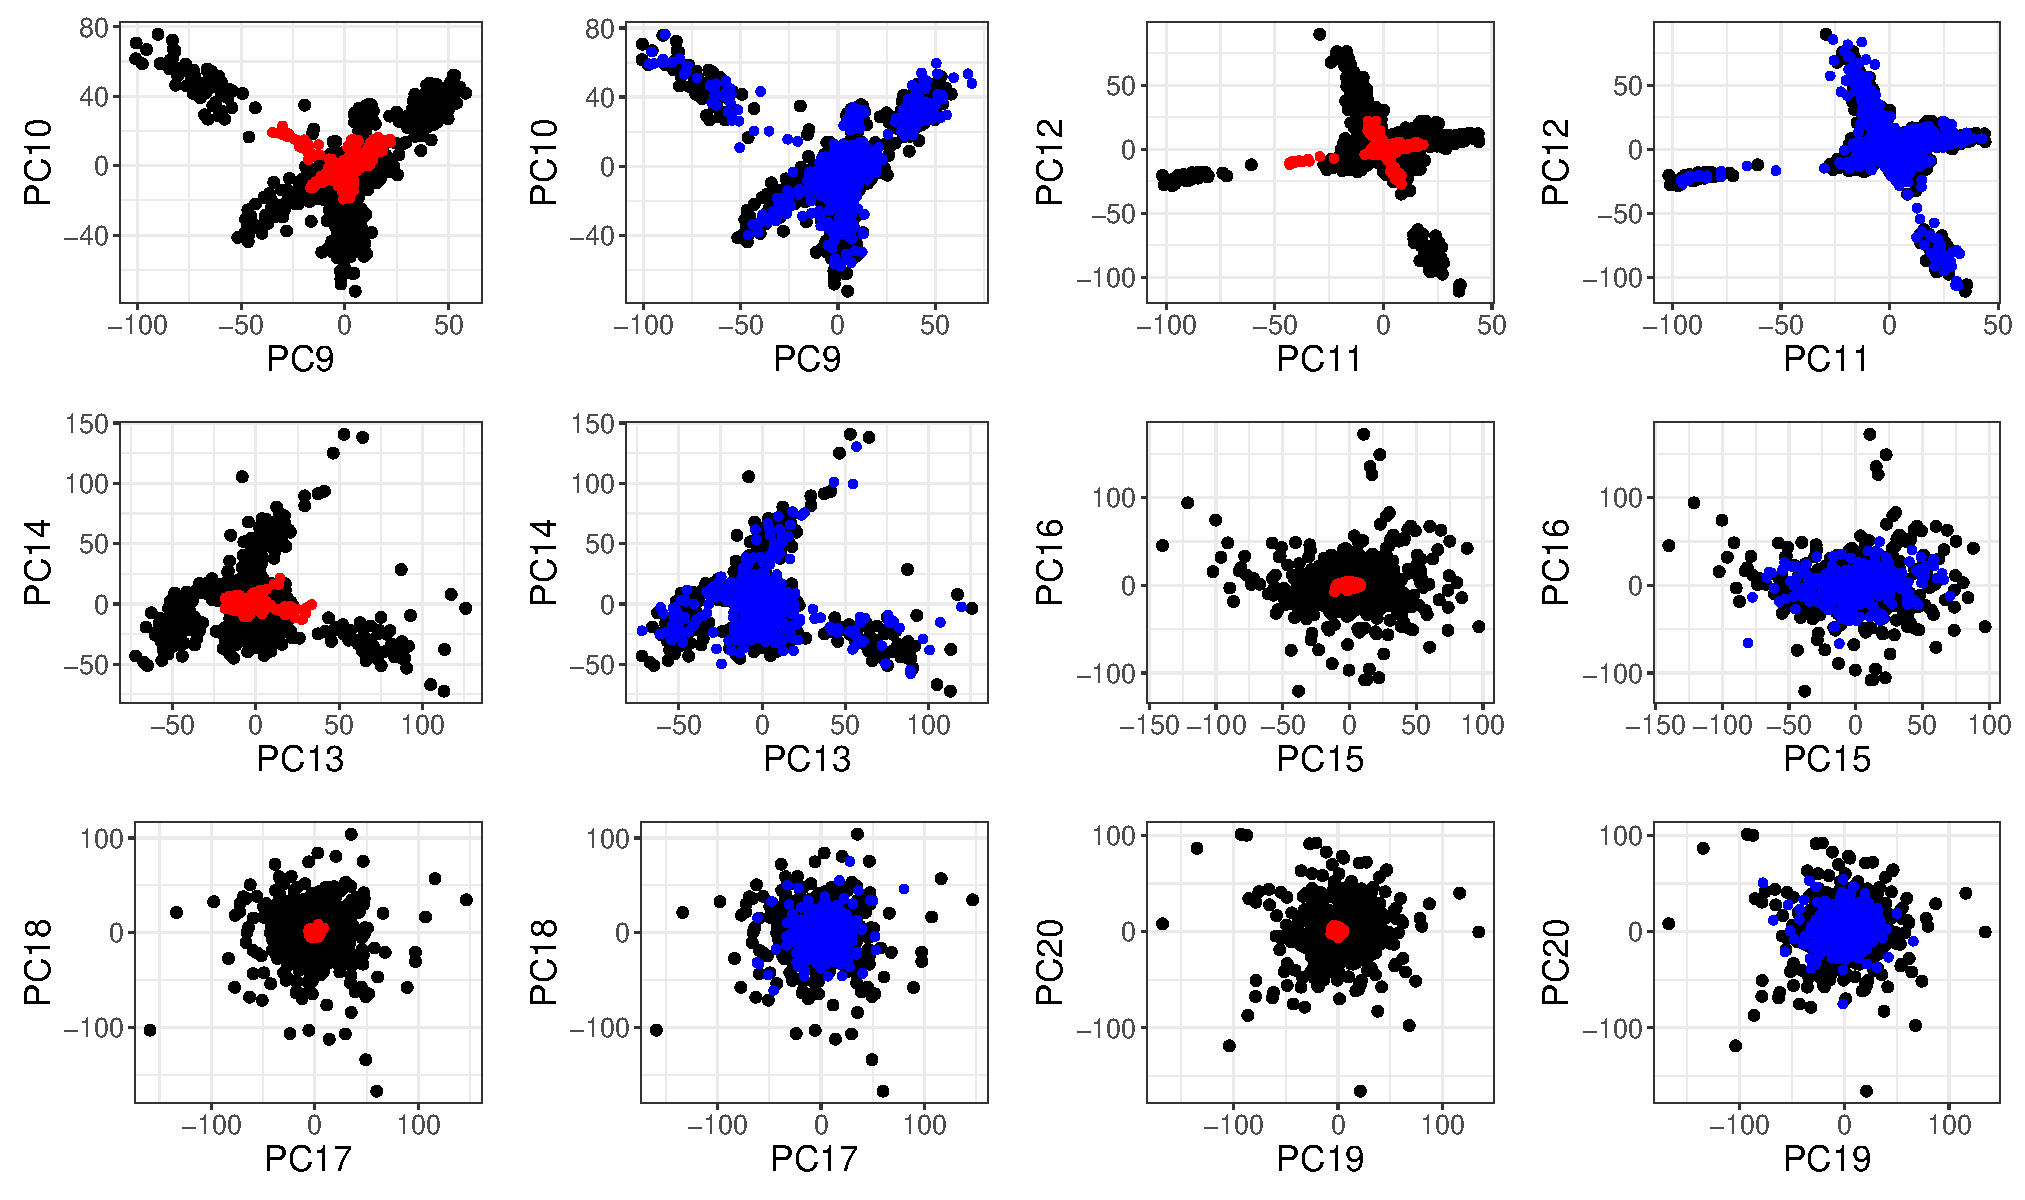
\includegraphics[width=0.9\textwidth]{proj1000G-PC9-20.pdf}}
\caption{Principal Component (PC) scores 9 to 20 of the 1000 Genomes project.
Black points are the 60\% individuals used for computing PCA.
Red points are the 40\% remaining individuals, projected by simply multiplying their genotypes by the corresponding PC loadings.
Blue points are the 40\% remaining individuals, projected using the Online Augmentation, Decomposition, and Procrustes (OADP) transformation.
Estimated shrinkage coefficients (comparing red and blue points) for these PCs are 2.79, 3.14 (PC10), 3.64, 3.18, 2.47, 3.88, 5.31, 5.84, 3.45, 6.55, 3.68 and 6.70 (PC20).
\label{fig:proj1000G-2}}
\end{figure}

\vspace*{1em}

\begin{figure}[!htpb]
\centerline{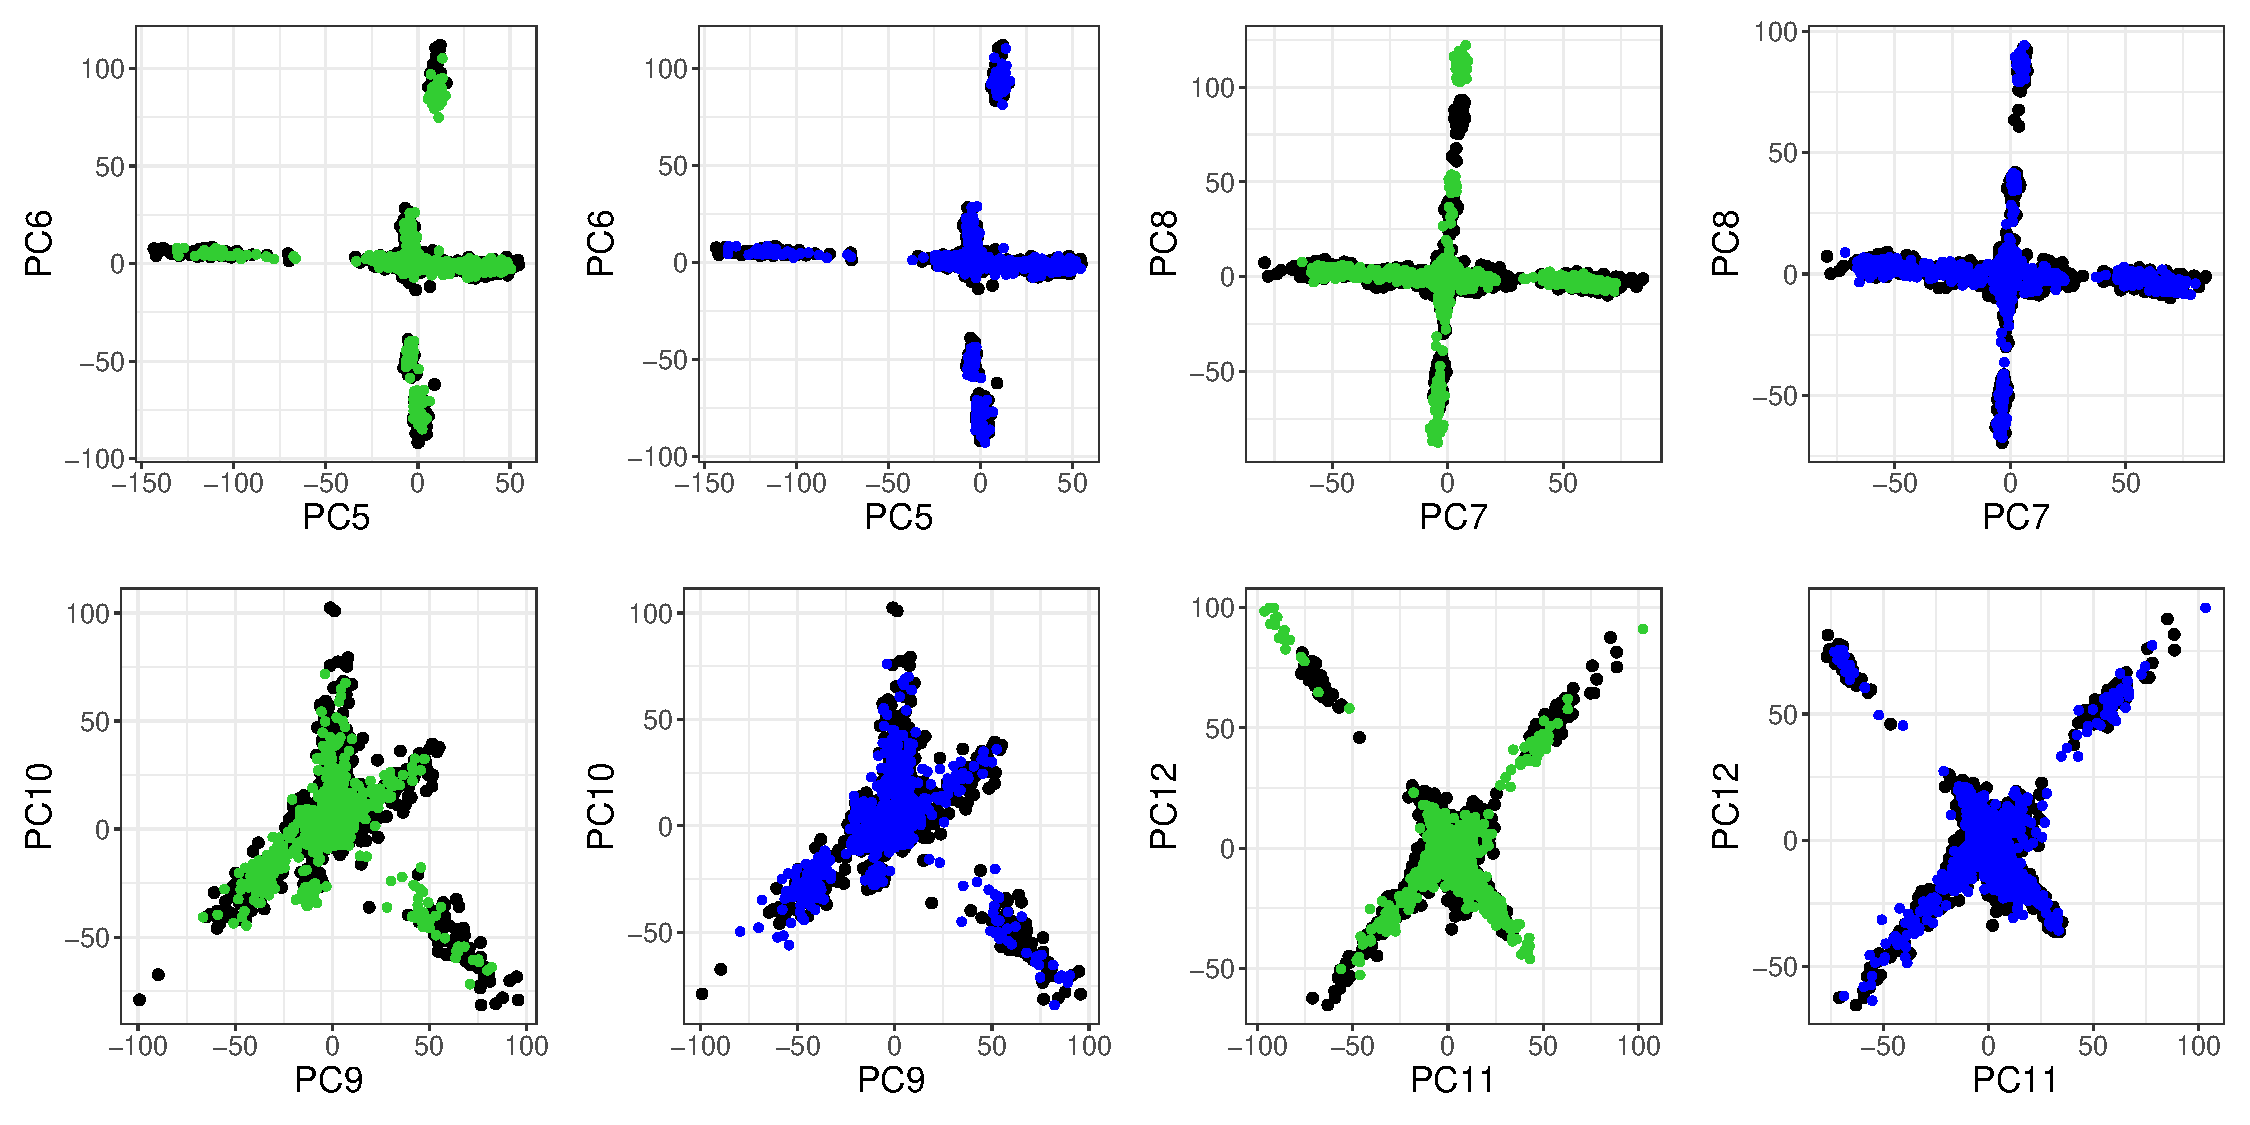
\includegraphics[width=0.9\textwidth]{proj1000G-PC5-12.pdf}}
\caption{Principal Component (PC) scores 5 to 12 of the 1000 Genomes project.
Black points are the 60\% individuals used for computing PCA.
Green points are the 40\% remaining individuals, projected by multiplying their genotypes by the corresponding PC loadings, further corrected using theoritical asymptotic shrinkage factors (values for the first 12 PCs: 1.01 (PC1), 1.02, 1.07, 1.10, 1.43 (PC5), 1.54, 1.74, 1.79, 2.47, 2.77 (PC10), 2.84 and 3.15).
Blue points are the 40\% remaining individuals, projected using the Online Augmentation, Decomposition, and Procrustes (OADP) transformation.
\label{fig:proj1000G-3}}
\end{figure}

\begin{figure}[!htpb]
\centerline{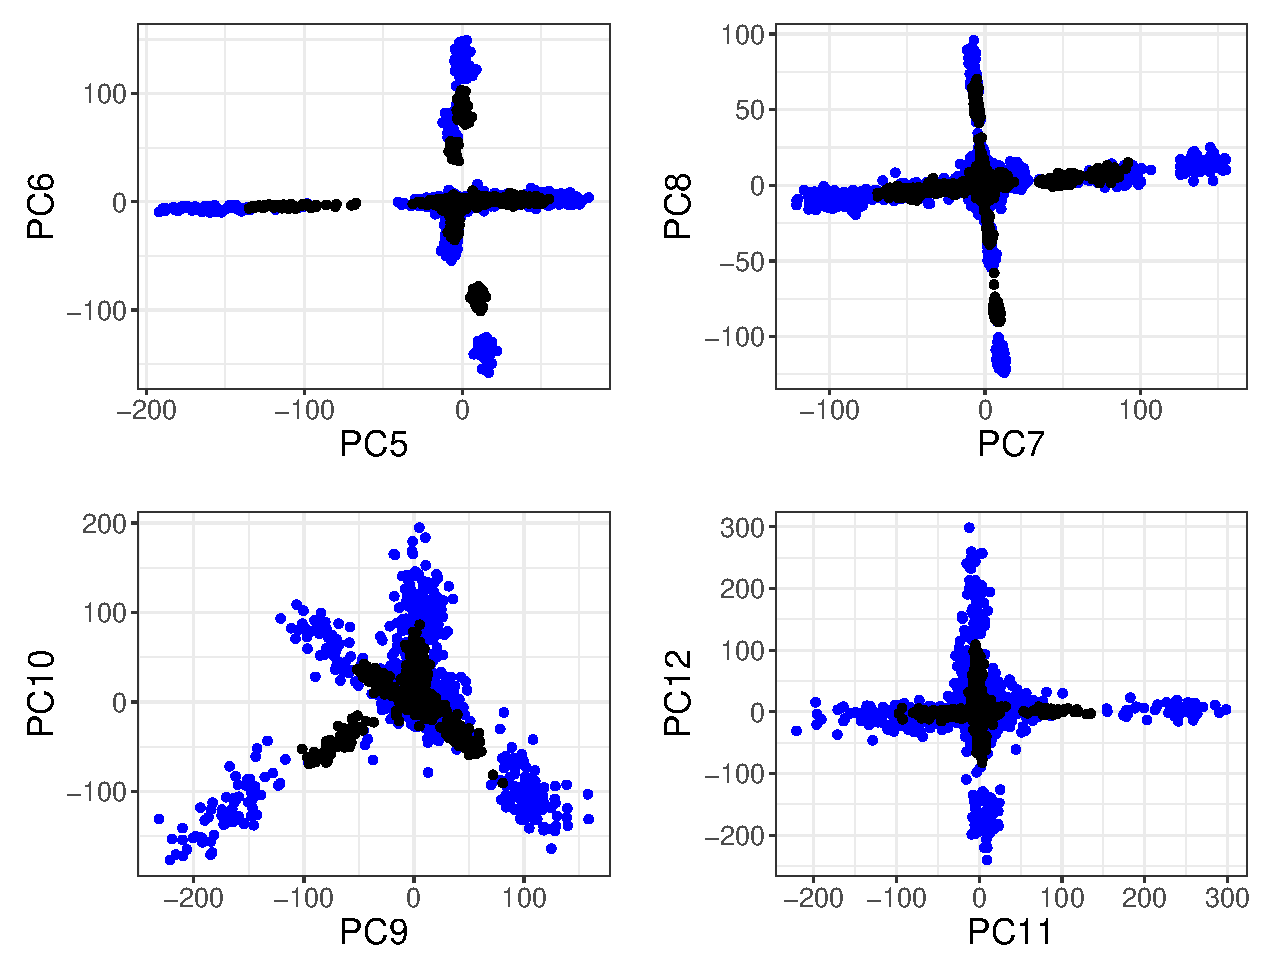
\includegraphics[width=0.9\textwidth]{proj1000G-related.pdf}}
\caption{Principal Component (PC) scores 5 to 12 of the 1000 Genomes project.
Black points are the 60\% individuals used for computing PCA.
Blue points are the same 60\% individuals, projected using the Online Augmentation, Decomposition, and Procrustes (OADP) transformation.
\label{fig:proj1000G-4}}
\end{figure}

\begin{figure}[!htpb]
\centerline{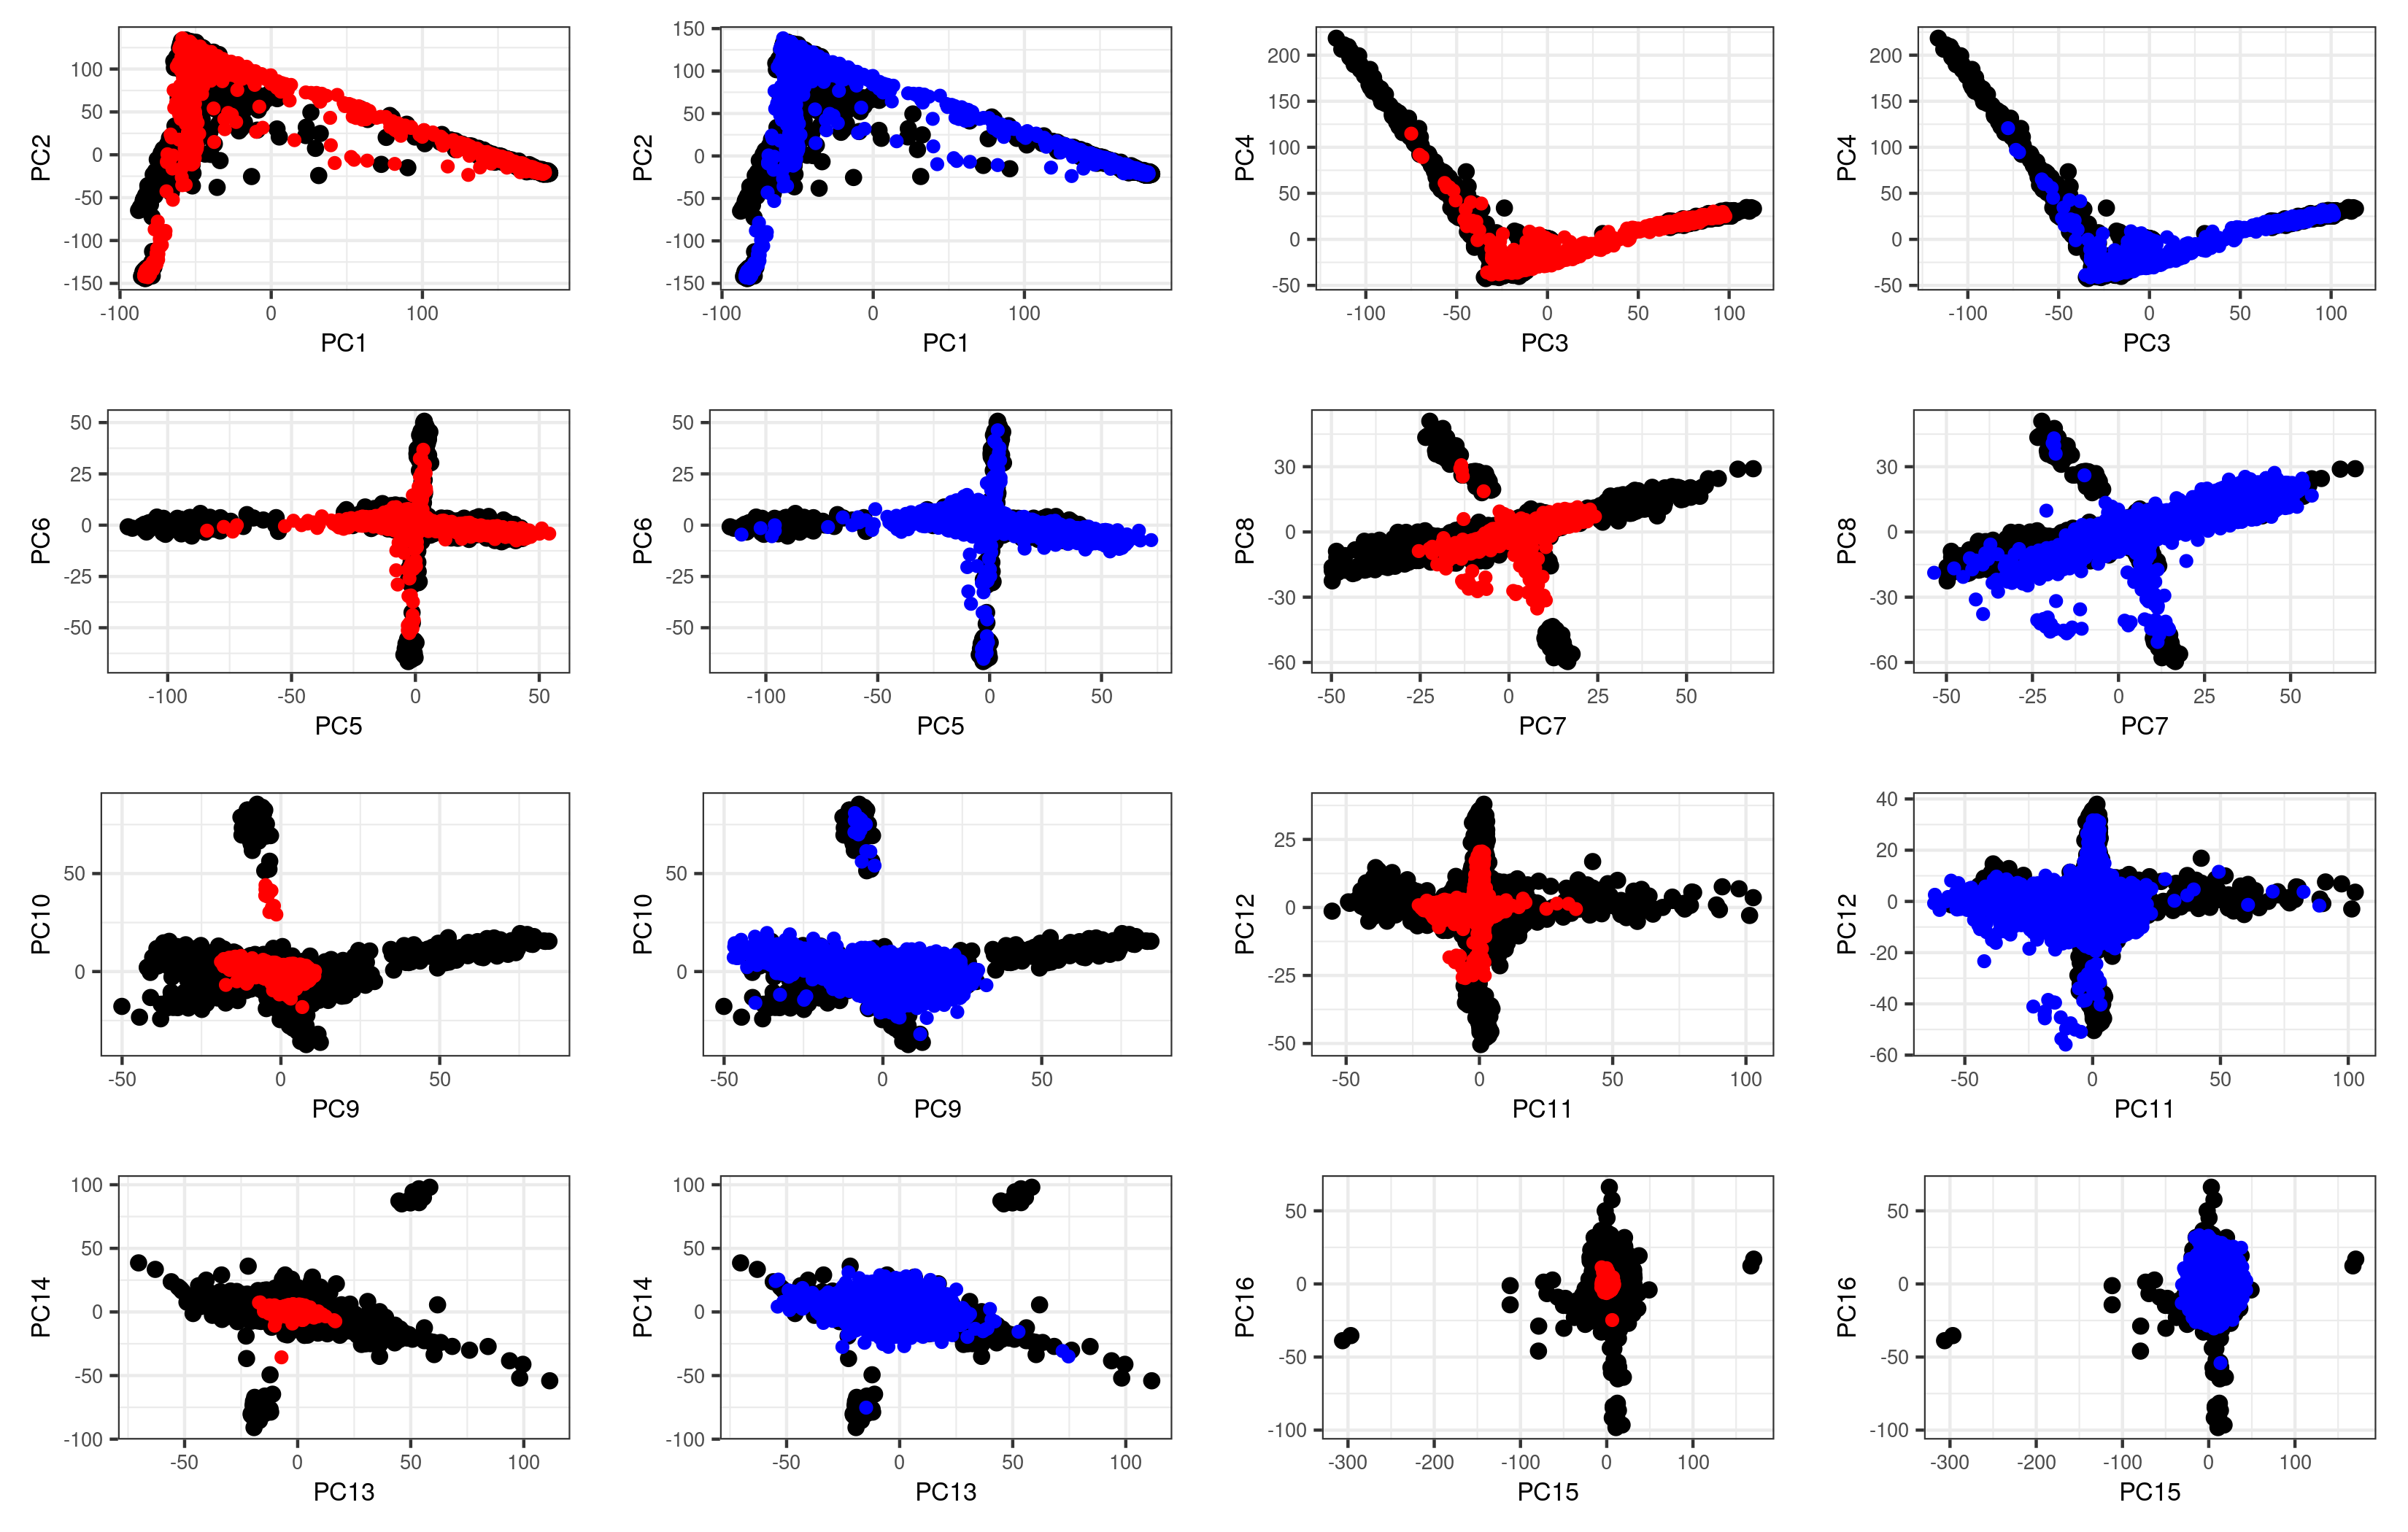
\includegraphics[width=0.9\textwidth]{proj1000G-UKBB.png}}
\caption{Principal Component (PC) scores 1 to 16 of the 1000 Genomes project and projected individuals from the UK Biobank.
Black points are PC scores of 1000G individuals used for computing PCA.
Red points are the individuals from UKBB, projected by simply multiplying their genotypes by the corresponding PC loadings.
Blue points are the 488,371 individuals from the UK Biobank, projected using the Online Augmentation, Decomposition, and Procrustes (OADP) transformation. 
Estimated shrinkage coefficients (comparing red and blue points) for the first 20 PCs are 1.01 (PC1), 1.02, 1.06, 1.08, 1.36 (PC5), 1.82, 2.33, 2.36, 2.78, 2.84 (PC10), 2.99, 3.51, 4.38, 4.67, 4.99, 5.31, 5.74, 6.55, 6.71 and 6.75 (PC20).
Note that only 20,000 random projected individuals are represented in this plot.
\label{fig:proj1000G-5}}
\end{figure}

\begin{figure}[!htpb]
\centerline{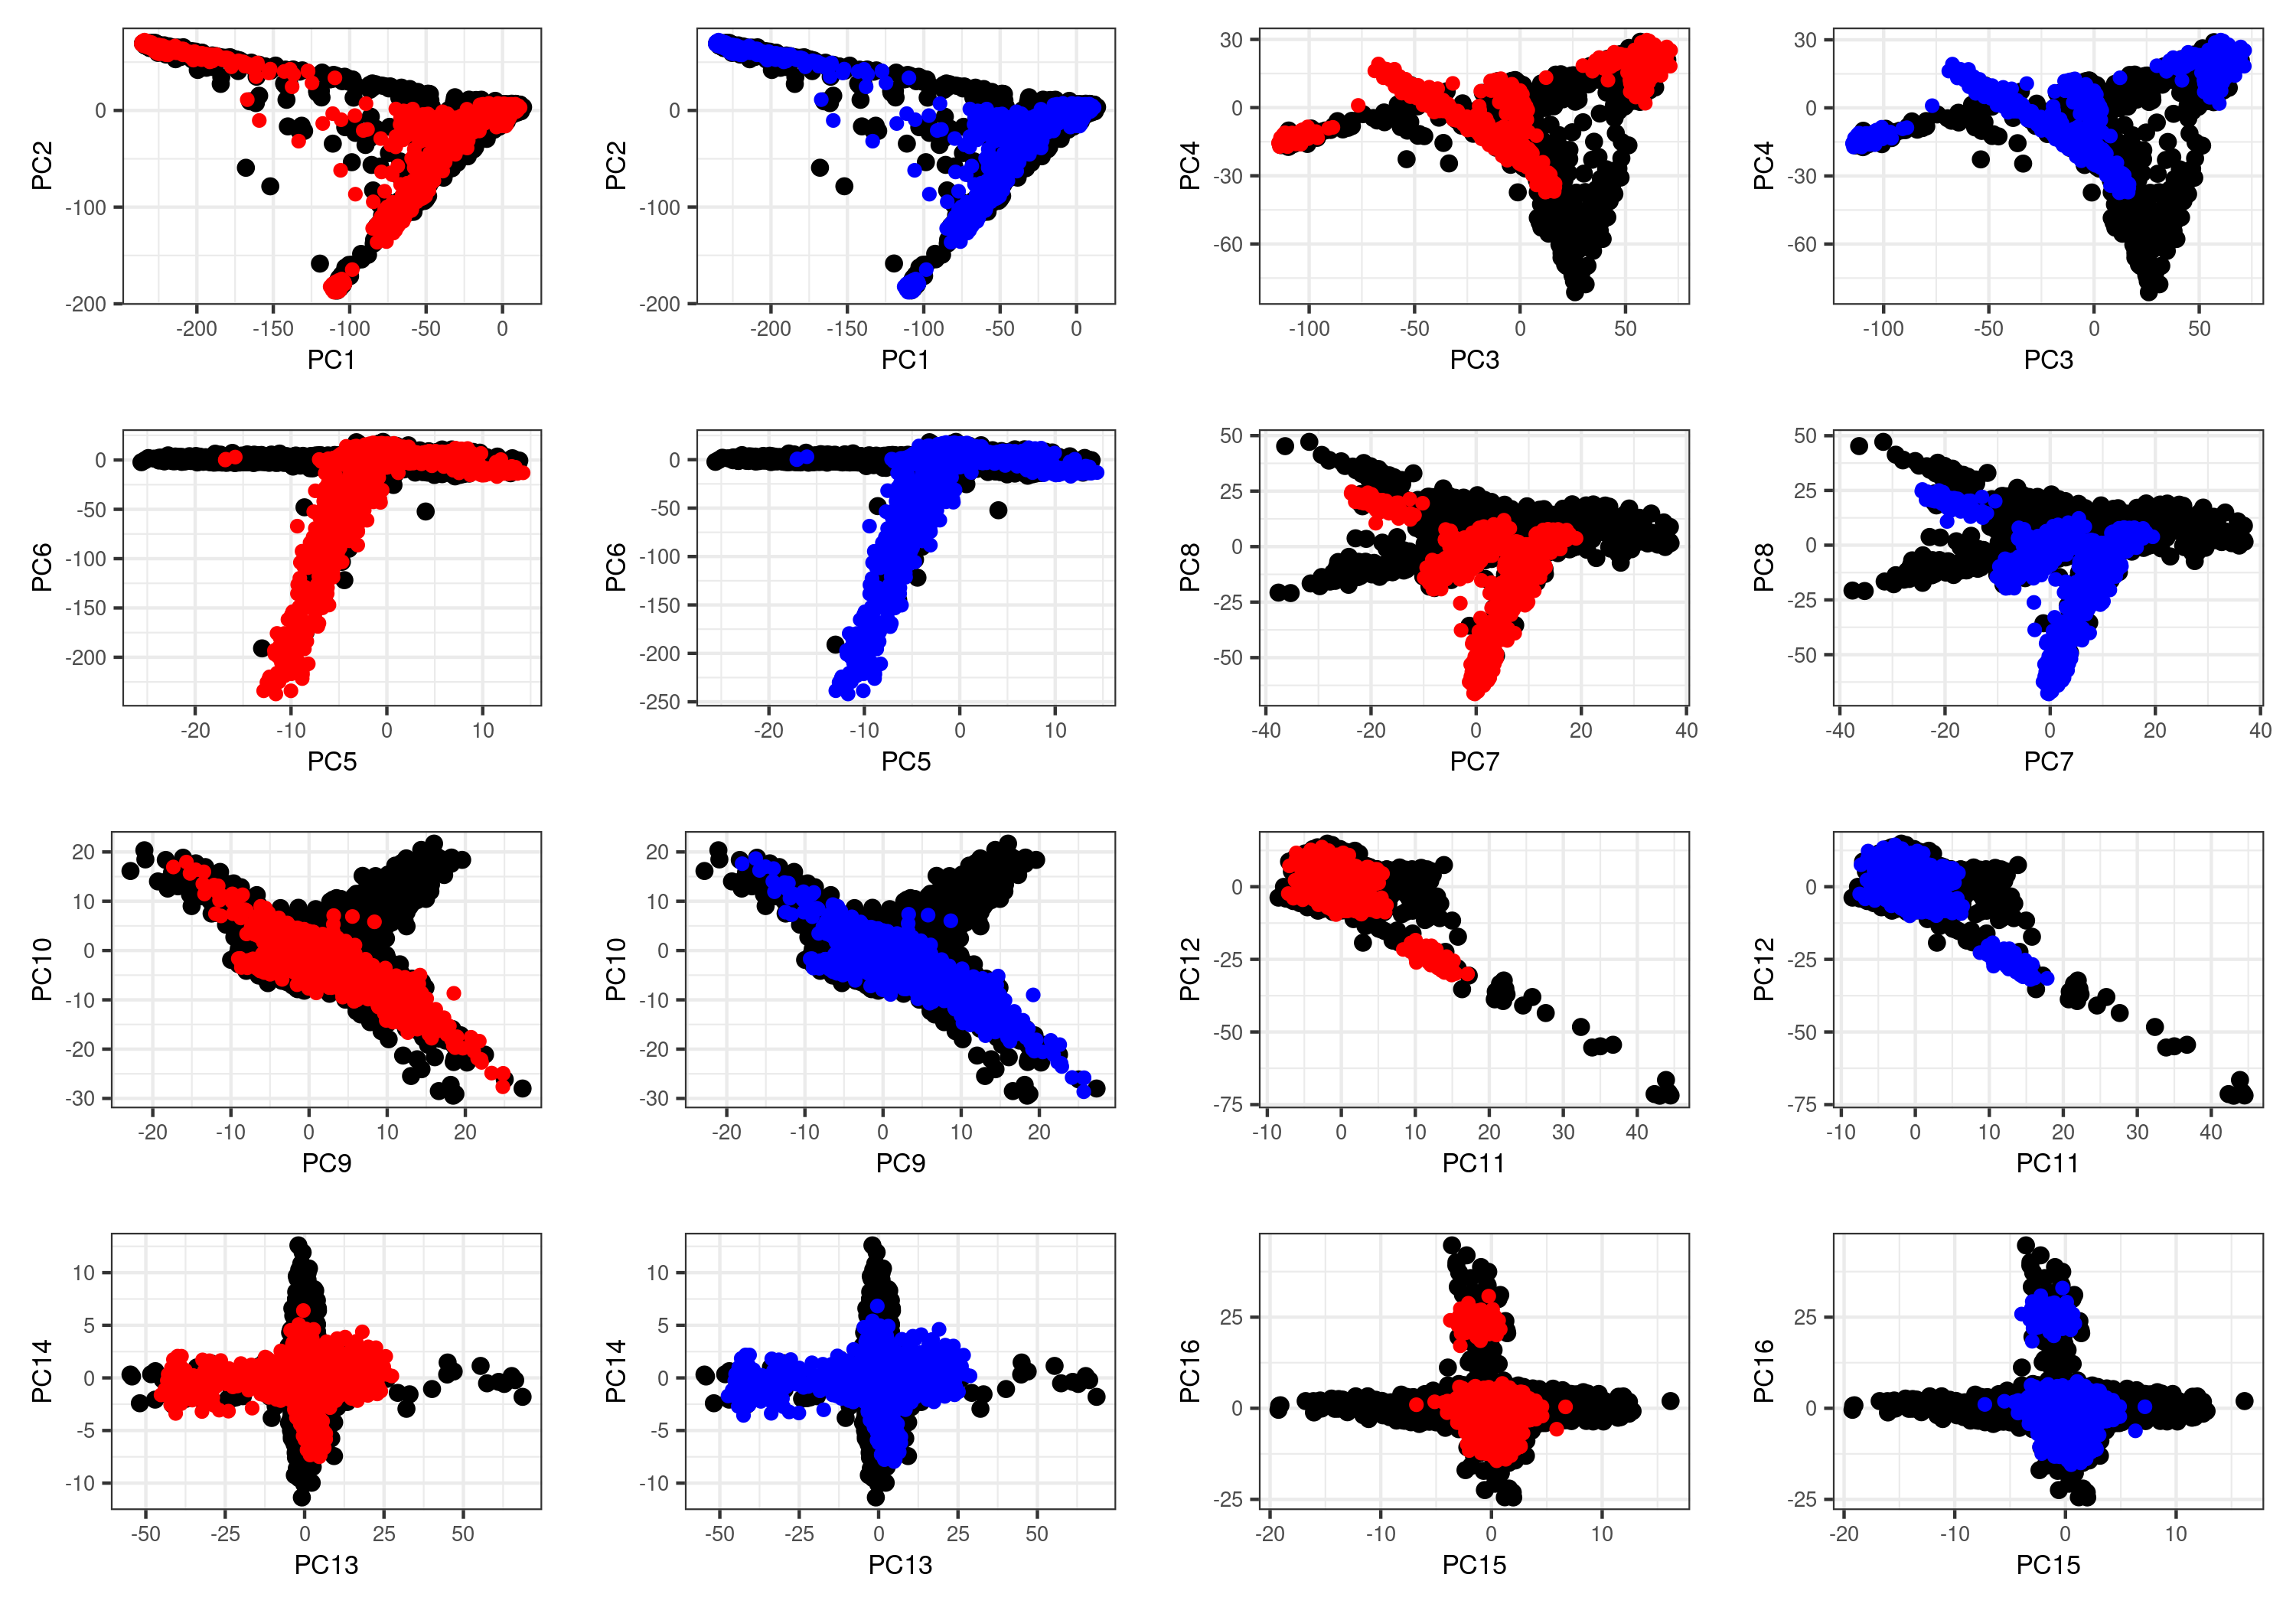
\includegraphics[width=0.8\textwidth]{proj1000G-UKBB2.png}}
\caption{Principal Component (PC) scores 1 to 16 from the UK Biobank and projected individuals of the 1000 Genomes (1000G) project.
Black points are the UK Biobank individuals used for computing PCA.
Red points are the individuals from 1000G, projected by simply multiplying their genotypes by the corresponding PC loadings.
Blue points are the individuals from 1000G, projected using the Online Augmentation, Decomposition, and Procrustes (OADP) transformation.
Estimated shrinkage coefficients (comparing red and blue points) for the first 20 PCs are 1.00 (PC1), 1.00, 1.00, 1.01, 1.01 (PC5), 1.02, 1.03, 1.03, 1.04, 1.04 (PC10), 1.04, 1.05, 1.05, 1.06, 1.07, 1.07, 1.08, 1.08, 1.08 and 1.08 (PC20).
\label{fig:proj1000G-6}}
\end{figure}

%%%%%%%%%%%%%%%%%%%%%%%%%%%%%%%%%%%%%%%%%%%%%%%%%%%%%%%%%%%%%%%%%%%%%%%%%%%%%%%%

\newpage

\begin{figure}[!htpb]
\centerline{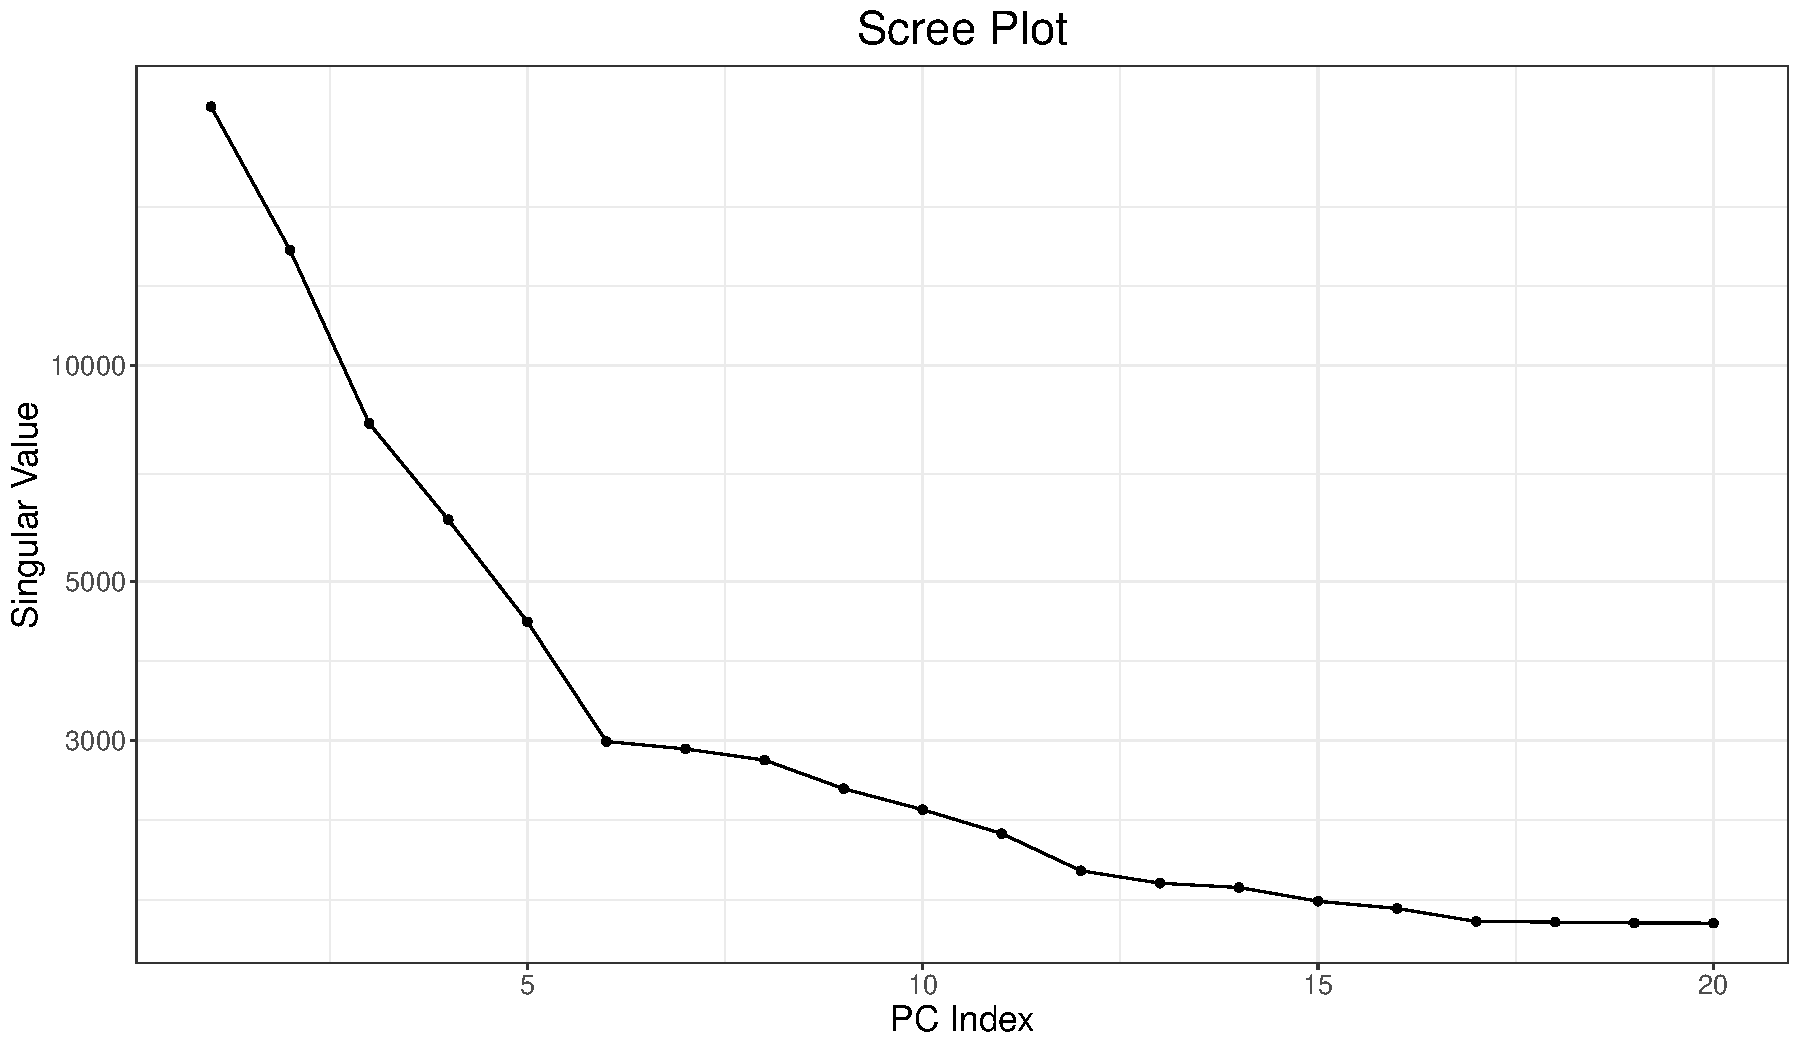
\includegraphics[width=0.8\textwidth]{UKBB-screeplot.pdf}}
\caption{Scree plot: plot of singular values computed on the UK Biobank using \texttt{bed\_autoSVD}.
\label{fig:UKBB-screeplot}}
\end{figure}

\begin{figure}[!htpb]
\centerline{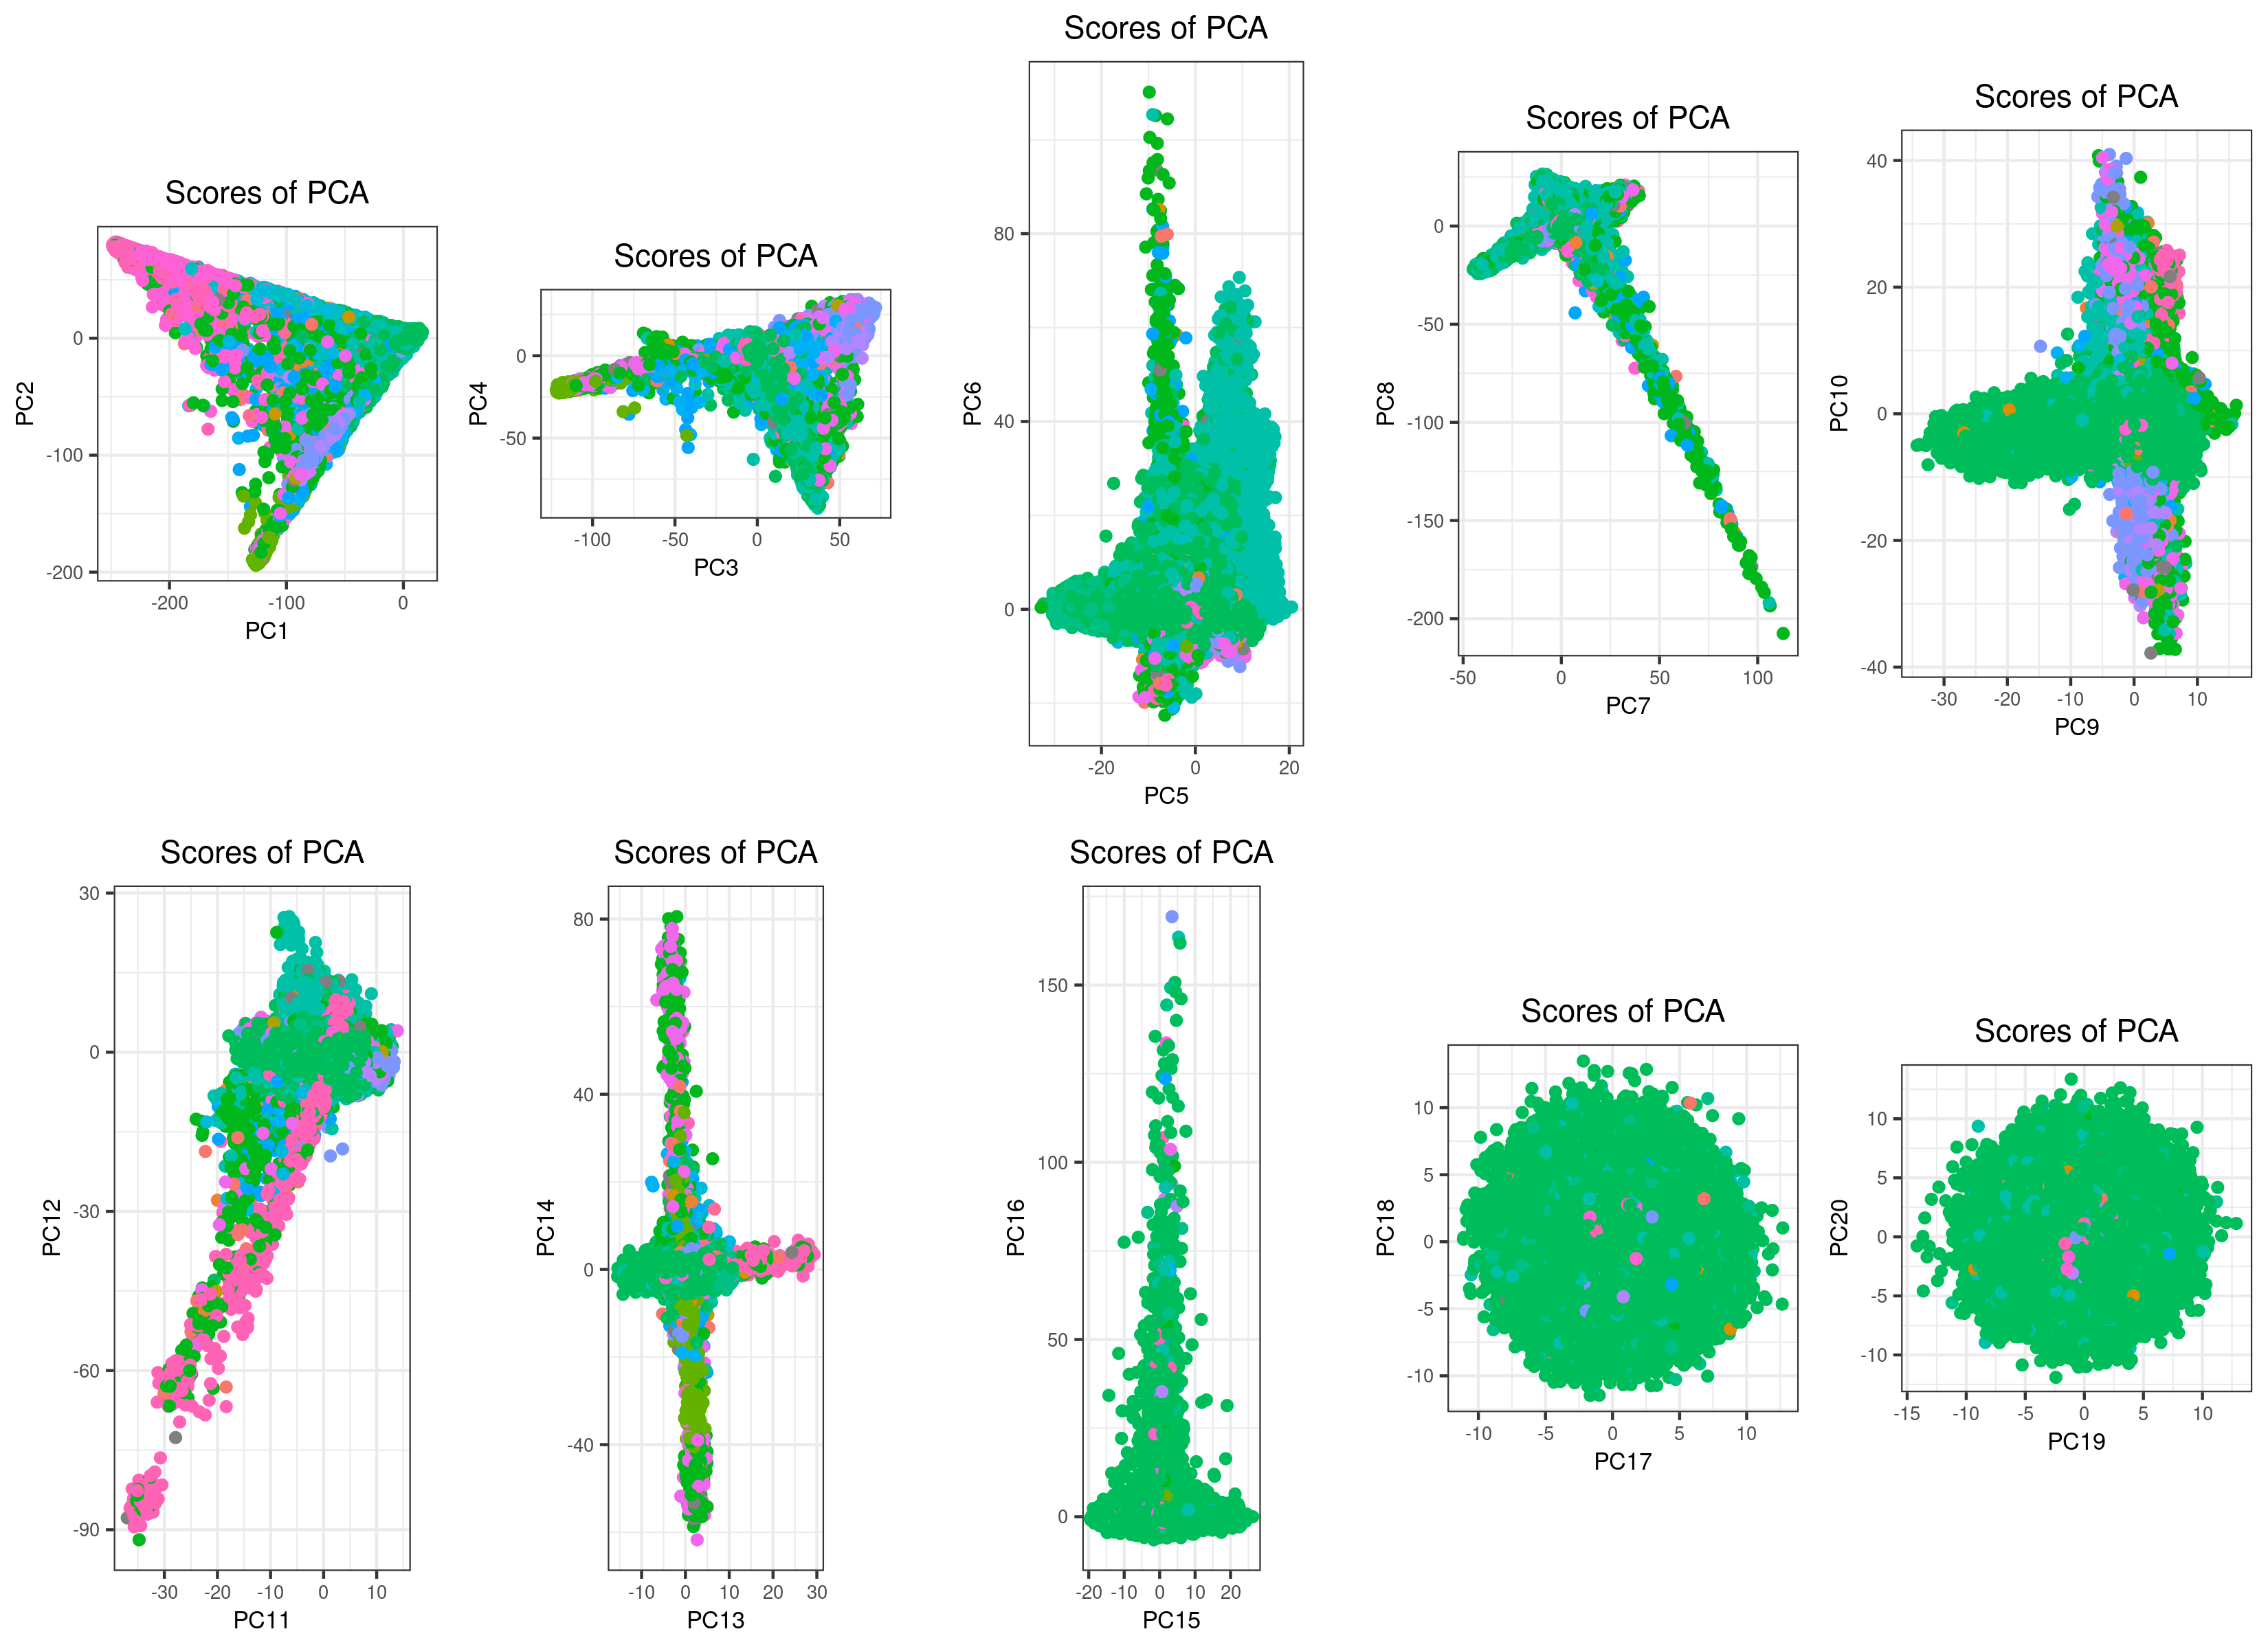
\includegraphics[width=0.9\textwidth]{UKBB-PC1-20.png}}
\caption{Principal Component (PC) scores 1 to 20 computed on the UK Biobank using \texttt{bed\_autoSVD}.
Different colors represent different self-reported ancestries.
\label{fig:UKBB-scores}}
\end{figure}

\begin{figure}[!htpb]
\centerline{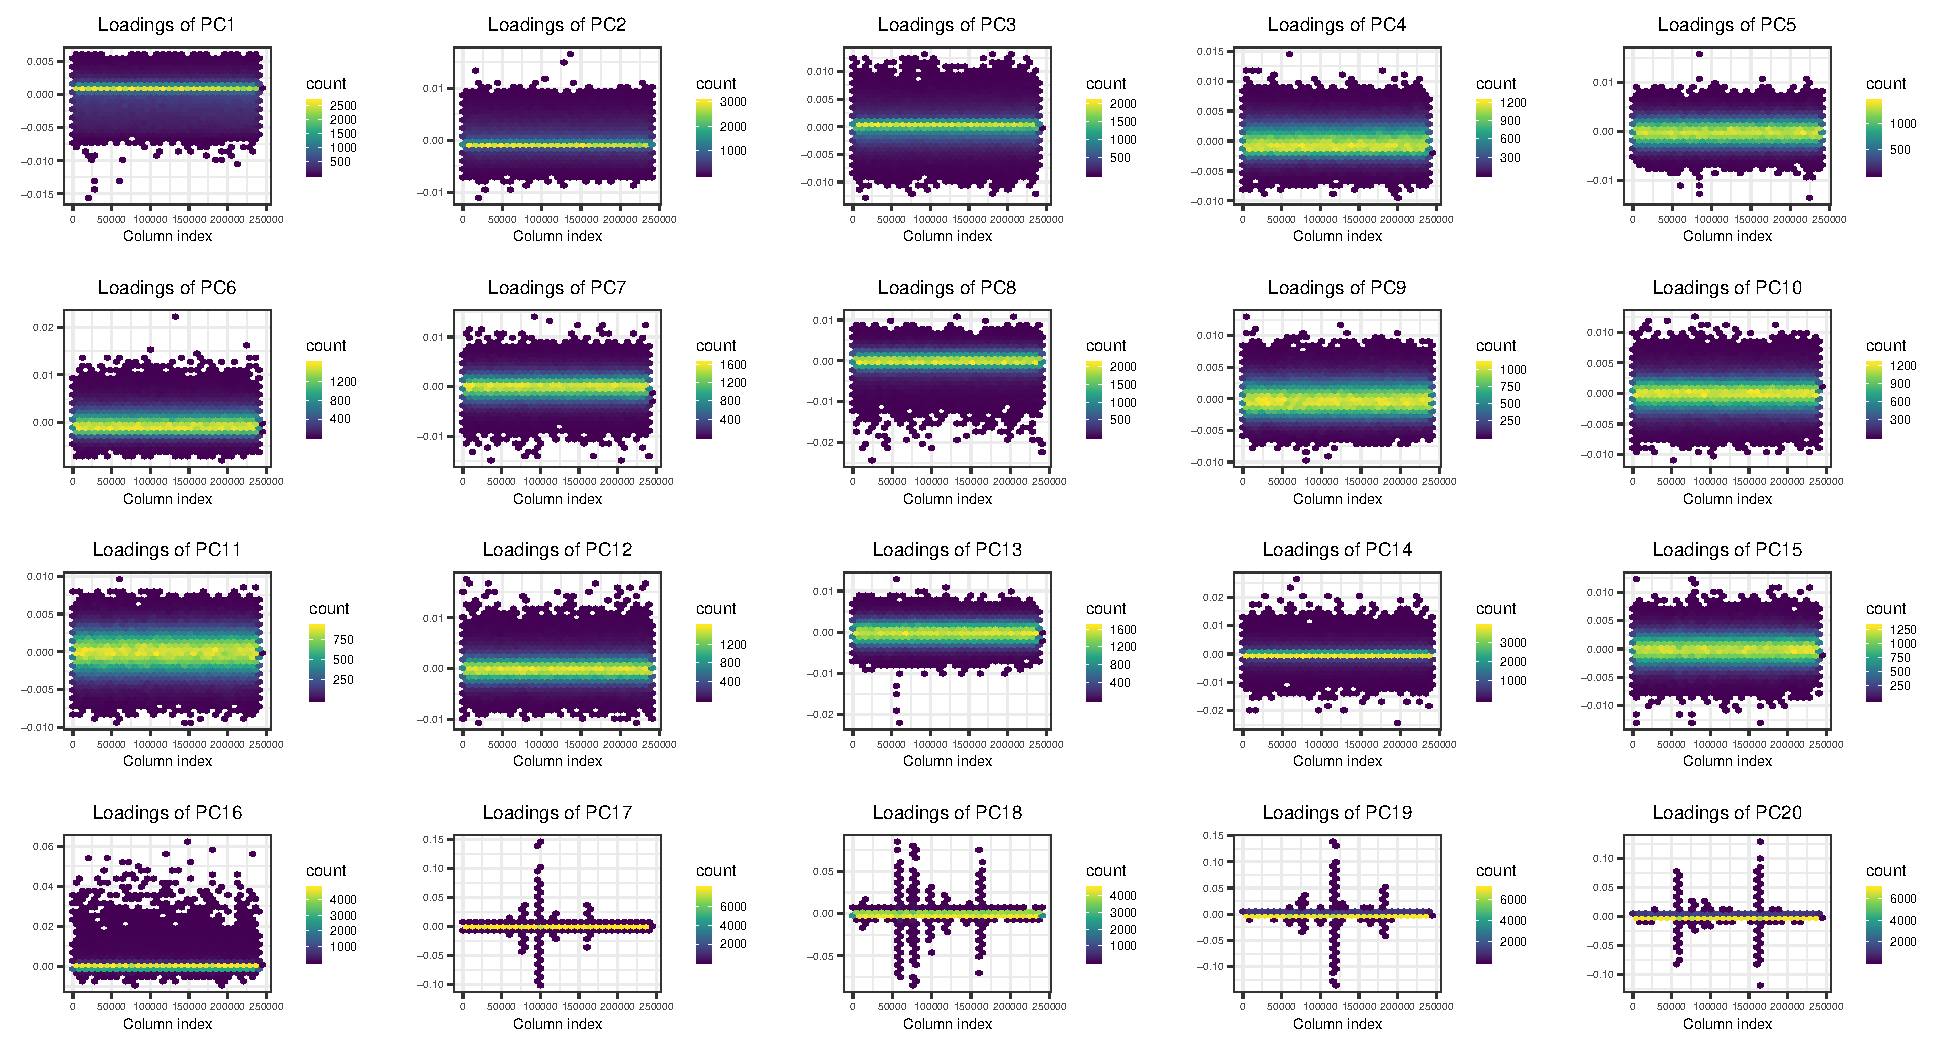
\includegraphics[width=0.9\textwidth]{UKBB-loadings.pdf}}
\caption{Principal Component (PC) loadings 1 to 20 computed on the UK Biobank using \texttt{bed\_autoSVD}.
\label{fig:UKBB-loadings}}
\end{figure}

%%%%%%%%%%%%%%%%%%%%%%%%%%%%%%%%%%%%%%%%%%%%%%%%%%%%%%%%%%%%%%%%%%%%%%%%%%%%%%%%

\begin{figure}[!htpb]
\centerline{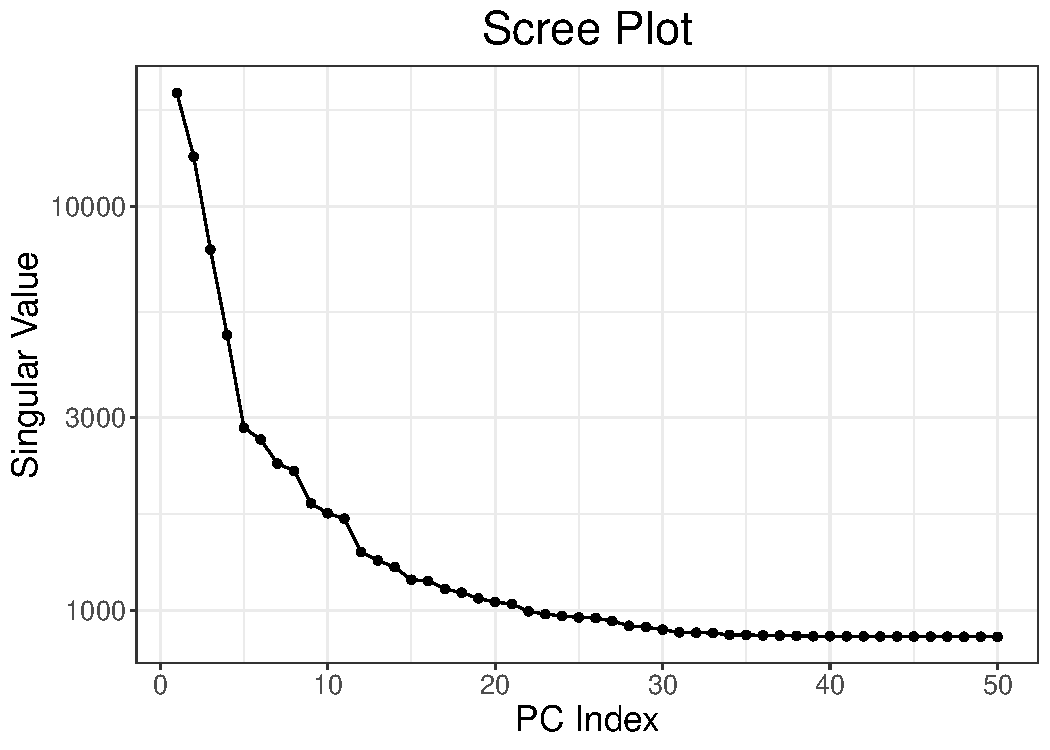
\includegraphics[width=0.8\textwidth]{UKBB-screeplot-restricted.pdf}}
\caption{Scree plot: plot of singular values computed on the UK Biobank using 48,942 individuals of diverse ancestries. These individuals are the ones resulting from removing all related individuals and randomly subsampling the British and Irish individuals.
\label{fig:UKBB-screeplot2}}
\end{figure}

\begin{figure}[!htpb]
\centerline{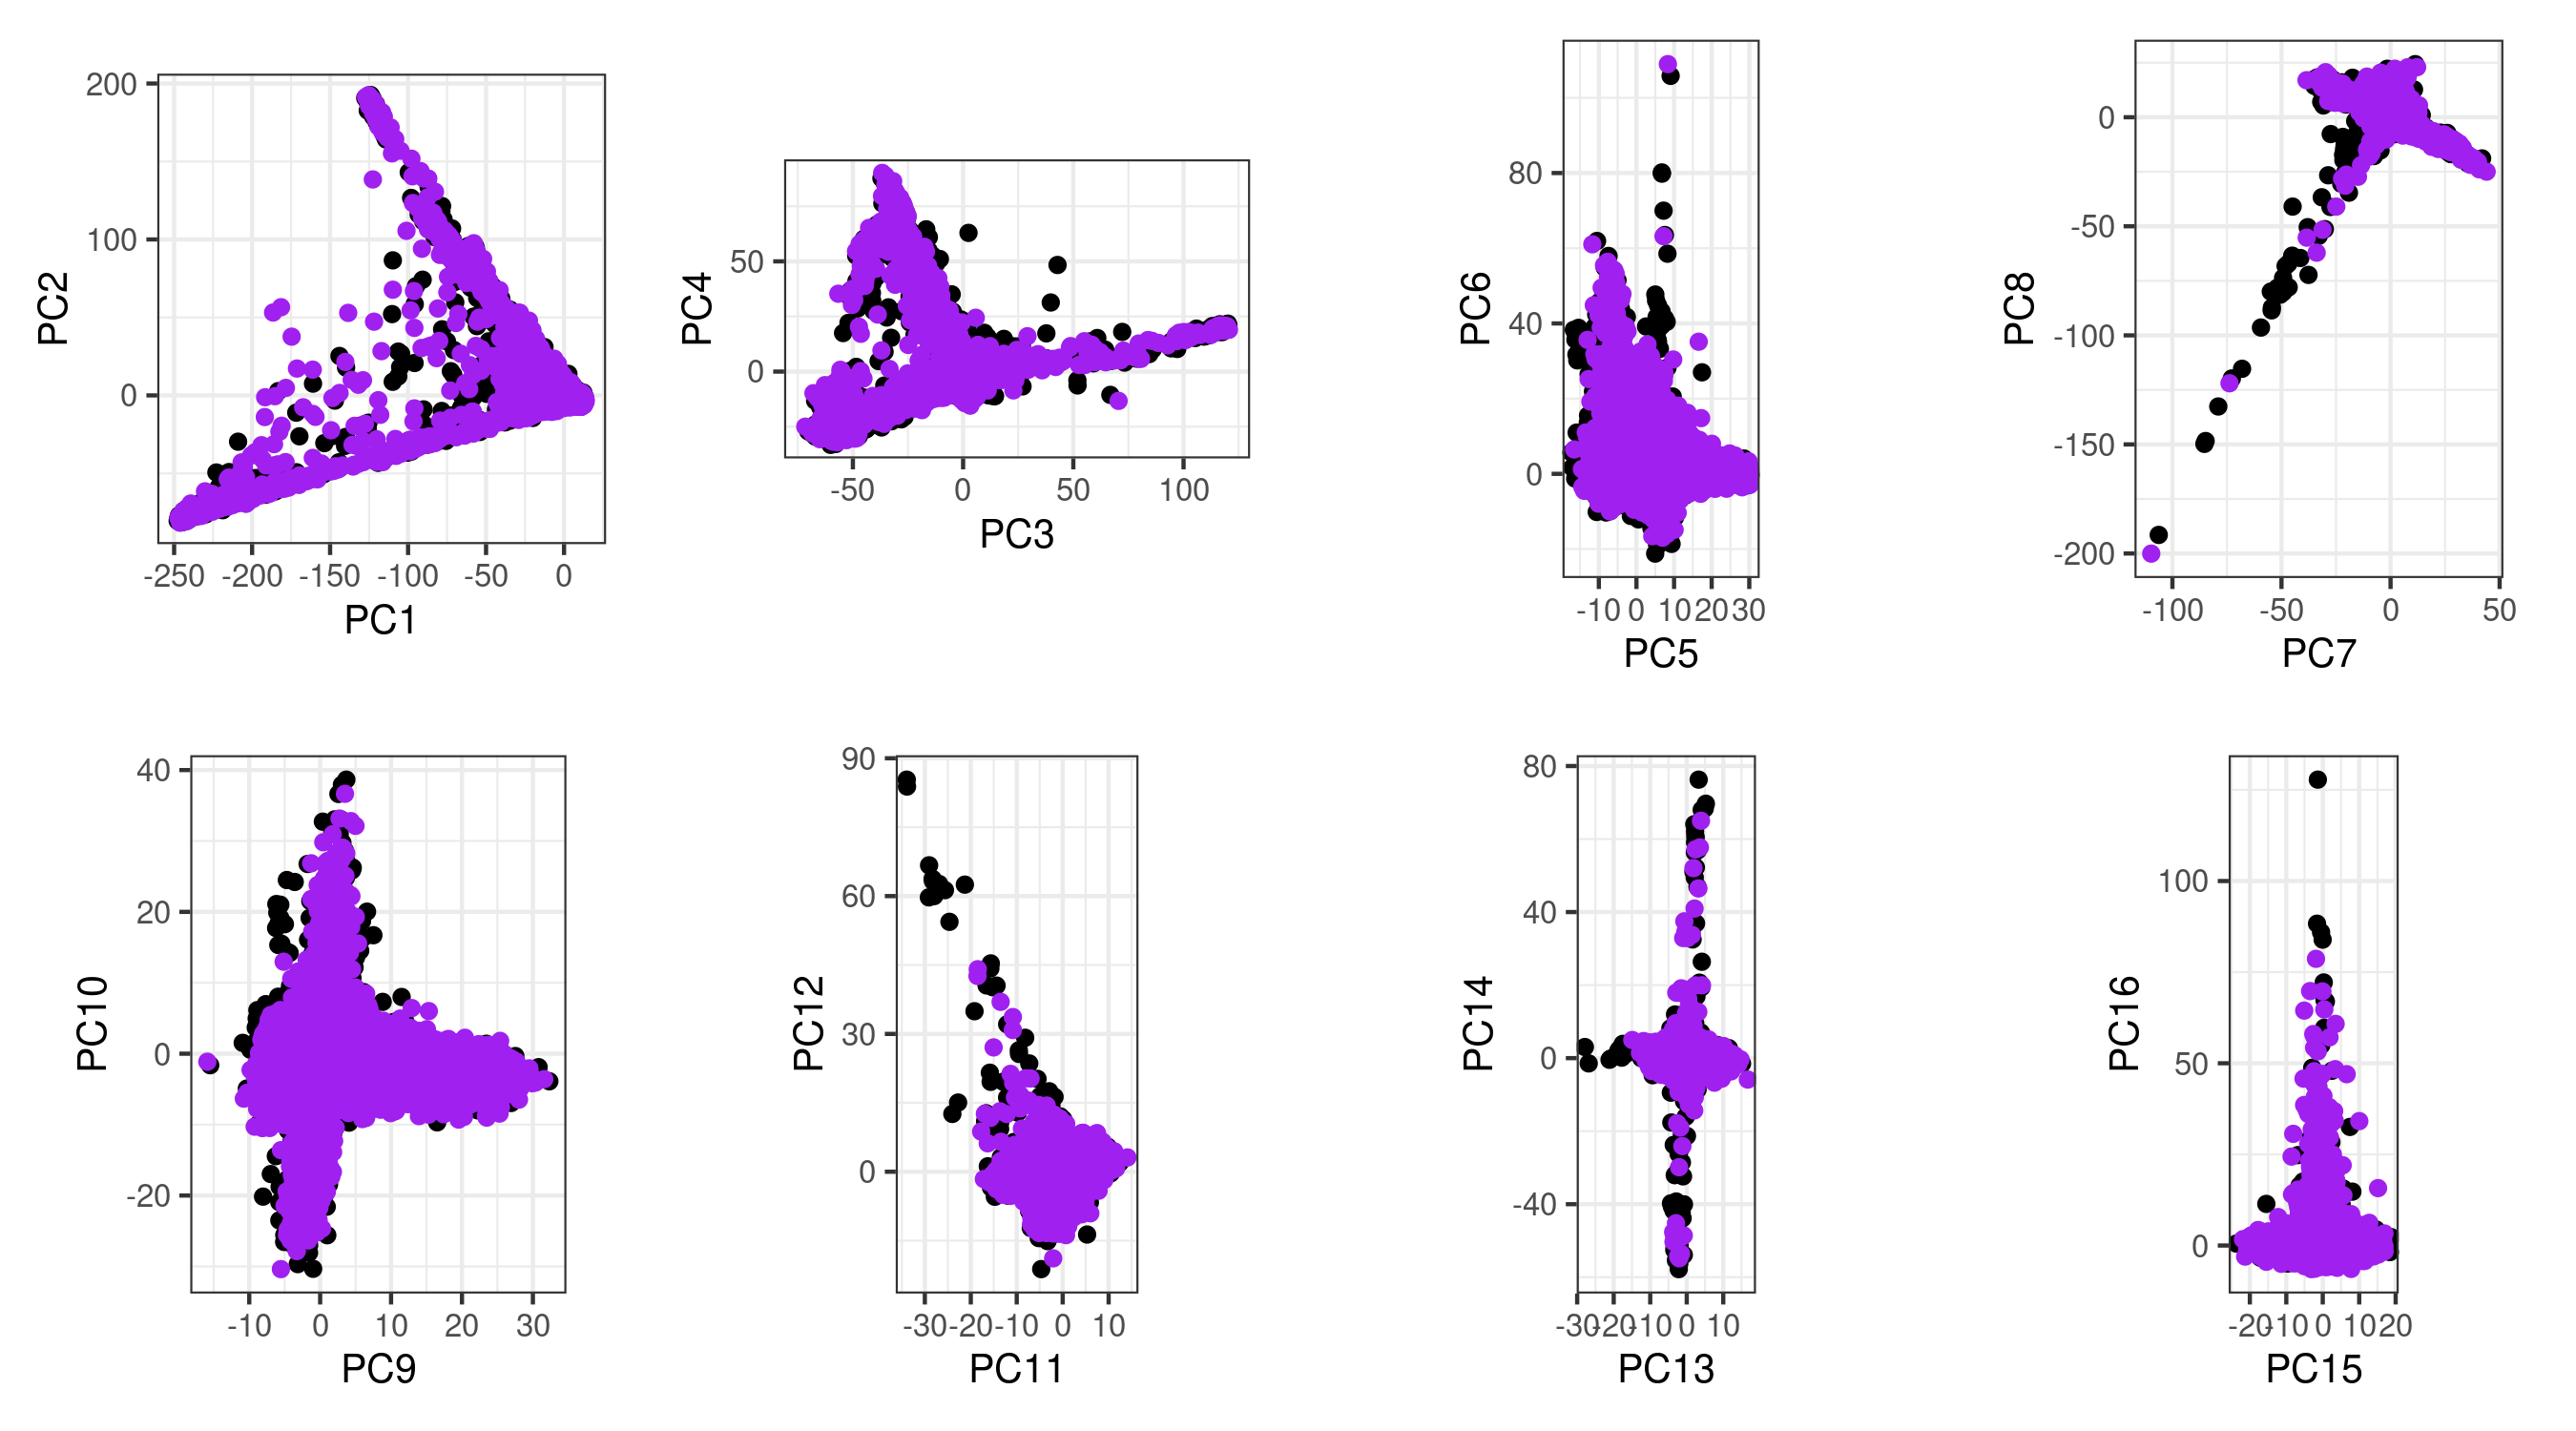
\includegraphics[width=0.9\textwidth]{projUKBB-related.png}}
\caption{Principal Component (PC) scores 27 to 50 of the UK Biobank.
Black points are the 48,942 individuals of diverse ancestries () used for computing PCA.
These individuals are the ones resulting from removing all related individuals and randomly subsampling the British and Irish individuals.
Red points are the remaining UKBB individuals, projected by simply multiplying their genotypes by the corresponding PC loadings.
Blue points are the remaining UKBB individuals, projected using the Online Augmentation, Decomposition, and Procrustes (OADP) transformation.
Note that only 20,000 random projected individuals are represented in this plot.
\label{fig:projUKBB-related}}
\end{figure}

%%%%%%%%%%%%%%%%%%%%%%%%%%%%%%%%%%%%%%%%%%%%%%%%%%%%%%%%%%%%%%%%%%%%%%%%%%%%%%%%

\end{document}
